% !BIB TS-program = biber

\RequirePackage[l2tabu,orthodox]{nag}

% TODO: decide if one-sided/two-sided
%\documentclass[headsepline,footsepline,footinclude=false,fontsize=11pt,paper=a4,listof=totoc,bibliography=totoc,BCOR=12mm,DIV=12]{scrbook} % two-sided
\documentclass[headsepline,footsepline,footinclude=false,oneside,fontsize=11pt,paper=a4,listof=totoc,bibliography=totoc]{scrbook} % one-sided

% TODO: change thesis information
\newcommand*{\getUniversity}{Technische Universität München}
\newcommand*{\getFaculty}{Informatics}
\newcommand*{\getDegree}{Informatics}
\newcommand*{\getSchool}{Computation, Information and Technology}
\newcommand*{\getTitle}{Seed Optimization for Directed Greybox Fuzzing in Commit-Change Testing}
\newcommand*{\getTitleGer}{Optimierung der Seed-Auswahl für Gerichtetes Greybox-Fuzzing beim Testen von Commit-Änderungen}
\newcommand*{\getAuthor}{Cevin Neubauer}
\newcommand*{\getDoctype}{Master's Thesis}
\newcommand*{\getSupervisor}{Prof. Dr. Alexander Pretschner}
\newcommand*{\getAdvisor}{Kohei Dozono, M.Sc.}
\newcommand*{\getKeywords}{keyword;another keyword;one more}
\newcommand*{\getSubmissionDate}{07.10.2026}
\newcommand*{\getSubmissionLocation}{Munich}

% TODO: change citation style in settings
\PassOptionsToPackage{table,svgnames,dvipsnames}{xcolor}

\usepackage[a-2u]{pdfx} % generate PDF/A: archival compliant, self-contained pdf
\usepackage[utf8]{inputenc}
\usepackage[T1]{fontenc}
\usepackage[sc]{mathpazo}
\usepackage[ngerman,american]{babel}
\usepackage[autostyle]{csquotes}
\usepackage[%
  backend=biber,
  url=false,
  style=alphabetic,
  maxnames=4,
  minnames=3,
  maxbibnames=99,
  giveninits,
  uniquename=init,
  style=acmnumeric]{biblatex}
\usepackage{graphicx}
\usepackage{scrhack} % necessary for listings package
\usepackage{listings}
\usepackage{booktabs}
\usepackage{lstautogobble}
\usepackage{tikz}
\usepackage{pgfplots}
\usepackage{pgfplotstable}
\usepackage{booktabs, threeparttable}
\usepackage[final]{microtype}
\usepackage{caption}
\usepackage[printonlyused]{acronym}
\usepackage{ifthen}
\usepackage{booktabs}
\usepackage{tabularx}
\usepackage{array}
\usepackage{makecell}
\usepackage{pifont}
\usepackage[colorinlistoftodos]{todonotes}
\usepackage[margin=1in]{geometry}
\usepackage{siunitx}


\usepackage{amsmath}

\usepackage{hyperref}
\usepackage[capitalise,nameinlink,noabbrev,sort&compress]{cleveref}

\usepackage{xcolor}
% 1. Define colors for diff highlight
% 1. Define colors for diff highlight & syntax
\definecolor{diffadd}{RGB}{230, 255, 230}
\definecolor{diffaddtext}{RGB}{0, 100, 0}
\definecolor{diffdel}{RGB}{255, 230, 230}
\definecolor{diffdeltext}{RGB}{139, 0, 0}
\definecolor{codegray}{rgb}{0.5,0.5,0.5}
\definecolor{keyblue}{rgb}{0.0, 0.0, 0.8}
\definecolor{strpurple}{rgb}{0.6, 0.0, 0.6}

% 2. Define the listing style
\lstdefinestyle{diffstyle}{
    language=C,
    basicstyle=\ttfamily\small,
    numbers=none,
    keepspaces=true,                 % <-- Crucial: preserves spaces
    columns=fullflexible,            % <-- Crucial: prevents awkward character spacing
    keywordstyle=\color{keyblue},
    commentstyle=\color{codegray}\itshape,
    stringstyle=\color{strpurple},
    showstringspaces=false,
    breaklines=true,
    frame=single,
    rulecolor=\color{black!20},
    escapeinside={(*@}{@*)}
}

\usepackage{tikz}
\usetikzlibrary{shapes.geometric, arrows.meta, positioning, fit, backgrounds}
\usepackage[most]{tcolorbox}

% Color definitions
\definecolor{controlcolor}{RGB}{40, 40, 40}
\definecolor{datacolor}{RGB}{0, 102, 204}
\definecolor{changesite}{RGB}{230, 80, 0}
\definecolor{crashsite}{RGB}{204, 0, 0}


\hypersetup{hidelinks} % removes colored boxes around references and links

% for fachschaft_print.pdf
\makeatletter
\if@twoside
	\typeout{TUM-Dev LaTeX-Thesis-Template: twoside}
\else
	\typeout{TUM-Dev LaTeX-Thesis-Template: oneside}
\fi
\makeatother

\addto\extrasamerican{
	\def\lstnumberautorefname{Line}
	\def\chapterautorefname{Chapter}
	\def\sectionautorefname{Section}
	\def\subsectionautorefname{Subsection}
	\def\subsubsectionautorefname{Subsubsection}
}

\addto\extrasngerman{
	\def\lstnumberautorefname{Zeile}
}

% Themes
\ifthenelse{\equal{\detokenize{dark}}{\jobname}}{%
  % Dark theme
  \newcommand{\bg}{black} % background
  \newcommand{\fg}{white} % foreground
  \usepackage[pagecolor=\bg]{pagecolor}
  \color{\fg}
}{%
  % Light theme
  \newcommand{\bg}{white} % background
  \newcommand{\fg}{black} % foreground
}


\bibliography{bibliography}

\setkomafont{disposition}{\normalfont\bfseries} % use serif font for headings
\linespread{1.05} % adjust line spread for mathpazo font

% Add table of contents to PDF bookmarks
\BeforeTOCHead[toc]{{\cleardoublepage\pdfbookmark[0]{\contentsname}{toc}}}

% Define TUM corporate design colors
% Taken from http://portal.mytum.de/corporatedesign/index_print/vorlagen/index_farben
\definecolor{TUMBlue}{HTML}{0065BD}
\definecolor{TUMSecondaryBlue}{HTML}{005293}
\definecolor{TUMSecondaryBlue2}{HTML}{003359}
\definecolor{TUMBlack}{HTML}{000000}
\definecolor{TUMWhite}{HTML}{FFFFFF}
\definecolor{TUMDarkGray}{HTML}{333333}
\definecolor{TUMGray}{HTML}{808080}
\definecolor{TUMLightGray}{HTML}{CCCCC6}
\definecolor{TUMAccentGray}{HTML}{DAD7CB}
\definecolor{TUMAccentOrange}{HTML}{E37222}
\definecolor{TUMAccentGreen}{HTML}{A2AD00}
\definecolor{TUMAccentLightBlue}{HTML}{98C6EA}
\definecolor{TUMAccentBlue}{HTML}{64A0C8}

% Settings for pgfplots
\pgfplotsset{compat=newest}
\pgfplotsset{
  % For available color names, see http://www.latextemplates.com/svgnames-colors
  cycle list={TUMBlue\\TUMAccentOrange\\TUMAccentGreen\\TUMSecondaryBlue2\\TUMDarkGray\\},
}

% Settings for lstlistings
\lstset{%
  basicstyle=\ttfamily,
  columns=fullflexible,
  autogobble,
  keywordstyle=\bfseries\color{TUMBlue},
  stringstyle=\color{TUMAccentGreen},
  captionpos=b
}

\newcommand{\bibliofont}{\normalfont}


\begin{document}

% Set page numbering to avoid "destination with the same identifier has been already used" warning for cover page.
% (see https://en.wikibooks.org/wiki/LaTeX/Hyperlinks#Problems_with_Links_and_Pages).
\pagenumbering{alph}
\input{pages/cover}

\frontmatter{}

\begin{titlepage}
  \centering

  \IfFileExists{logos/tum-\fg.pdf}{%
    \includegraphics[height=20mm]{logos/tum-\fg.pdf}
  }{%
    \vspace*{20mm}
  }

  \vspace{5mm}
  {\huge\MakeUppercase{School of \getSchool{} --- \getFaculty{}} \par}

  \vspace{5mm}
  {\large\MakeUppercase{\getUniversity{}} \par}

  \vspace{20mm}
  {\Large \getDoctype{} in \getDegree{} \par}

  \vspace{15mm}
  {\huge\bfseries \getTitle{} \par}

  \vspace{10mm}
  {\huge\bfseries \foreignlanguage{ngerman}{\getTitleGer{}} \par}

  \vspace{15mm}
  \begin{tabular}{l l}
    Author:          & \getAuthor{}         \\
    Examiner:      & \getSupervisor{}     \\
    Supervisor:         & \getAdvisor{}        \\
    Submission Date: & \getSubmissionDate{} \\
  \end{tabular}

  \IfFileExists{logos/faculty-\fg.pdf}{%
    \vfill{}
    \includegraphics[height=20mm]{logos/faculty-\fg.pdf}
  }{}
\end{titlepage}

% Uncomment the following line if you want to include a software usage table (see example in pages/software_used.tex)
\addcontentsline{toc}{chapter}{Software and AI tools used}

\thispagestyle{empty}

\begin{center}
    {\usekomafont{sectioning}\usekomafont{section} Software and AI tools used}
\end{center}
The following software was used when writing this thesis:
\begin{table}[h]
\centering
\small
\renewcommand{\arraystretch}{1.2}

\begin{tabular}{|p{3.5cm}|p{11.5cm}|}
\hline
\rowcolor{TUMSecondaryBlue}
\textcolor{TUMWhite}{\textbf{Used software}} &
\textcolor{TUMWhite}{\textbf{Details}} \\
\hline

{\raggedright ChatGPT by OpenAI\par}
&
\begin{tabular}{@{}p{2.2cm}p{8.9cm}@{}}

\textbf{Use case:} & Linguistic quality improvement \\
\textbf{Scope:} & Entire work \\

\end{tabular}
\\
\hline

{\raggedright Gemini by Google\par}
&
\begin{tabular}{@{}p{2.2cm}p{8.9cm}@{}}

\textbf{Use case:} & Research of related work and background references \\
\textbf{Scope:} & Background and related work chapters \\
\cline{1-2}
\end{tabular}
\\
\hline

{\raggedright Claude by Anthropic\par}
&
\begin{tabular}{@{}p{2.2cm}p{8.9cm}@{}}

\textbf{Use case:} & Linguistic quality improvement, review of written work,
program-code development, and figure design. \\
\textbf{Scope:} & Entire Work and related code \\
\cline{1-2}
\end{tabular}
\\
\hline

\end{tabular}

\caption{Software and AI tools used during the thesis}
\end{table}

\cleardoublepage{}
\input{pages/acknowledgments}
\chapter{\abstractname}

Fuzzing is a widely used technique for finding bugs, and most bugs found by continuous fuzzing are regressions introduced by recent code changes.
Such regressions are best caught before a change is merged, but fuzzing time is limited at that point, so the fuzzer's success depends heavily on its starting inputs, the seed corpus.
Existing approaches to generating seeds for regression fuzzing consider only the changed code, even though many bugs manifest in code that a change affects but does not modify.
They also generate seeds from scratch, although an existing corpus is often available.

This thesis proposes TACCO (Targeted Affected-Code Corpus Optimization), a pipeline that prepares a targeted seed corpus prior to fuzzing.
It first distills an existing corpus into the seeds most relevant to the code transitively affected by a commit.
A large language model agent then generates additional seeds aimed at affected code that the corpus does not yet cover.
The agent supplies well-formed inputs with the structure needed to reach that code, and the fuzzer mutates them into the malformed inputs that trigger the bug.

A first study on six projects from the BugOSS benchmark compared three starting corpora and two scopes of affected code.
Starting from the distilled corpus and targeting all affected code gave the best trade-off: compared with the original corpus, the resulting corpora increased coverage of affected code on five of six projects, by up to \num{52.3}~percentage points, while being \SIrange{42}{98}{\percent} smaller.
A second study ran \SI{8}{\hour} AFL++ campaigns on twelve projects, six of them not used for tuning.
Compared with the original corpus, the pipeline did not change how often regressions were found, and its median time to exposure was \SI{71}{\minute} shorter, or \SI{31}{\minute} including augmentation time, but this difference was not statistically significant.
These results show that distillation and augmentation yield smaller corpora that cover more affected code and suggest that such corpora can help expose regressions more quickly in time-limited settings.
\microtypesetup{protrusion=false}
\tableofcontents{}
\microtypesetup{protrusion=true}

\mainmatter{}

% !TeX root = ../main.tex
% Add the above to each chapter to make compiling the PDF easier in some editors.

\chapter{Introduction}\label{chapter:introduction}

\section{Motivation}
Four in every five bugs have been introduced by recent code changes (regeression)~\cite{zhuRegressionGreyboxFuzzing2021b}

Corpus Quality influence on fuzzing
% Focus: Works studying why initial seed quality, corpus distillation, and high initial branch coverage give downstream greybox mutators (like AFL++) a headstart. 
Overall to show: Corpus quality has a significant impact on fuzzing result. (Also explain what good quality means, and name studies that show that these qualities improve fuzzing)

First: Corpus influences fuzzing performance
- EvalFuzzTesting~\cite{kleesEvaluatingFuzzTesting2018} (Study investigated that experimental setups of most studies are flawed and names that a big factor is the initial seed selection, and then do experiments to show so)

Minimal Corpus is Good:
- Corpus Distillation for Effective Fuzzing \cite{herreraCorpusDistillationEffective2020} -> Distill Term!! (Study that compares full, distilled and "empty" (only header present) and comes to conclusion that for big corpora minimizing them is always good)
- Seed Selection for Successful Fuzzing \cite{herreraSeedSelectionSuccessful2021}

Targeted Corpus (Seed selection) is good:
ContinousFuzzingSAP, Bugoss~\cite{yooImprovingConfigurabilityUnitlevel2021}~\cite{kimBugOssBenchmarkRealworld2024} (Select based on functional Coverage)
DART corpus ~\cite{canakciTargetFuzzUsingDARTs2022} (Distance-based selection to target site of seeds)


I want to reframe things a  bit.

The setting is finding bugs introduced by commit changed code because here most bugs are introduces. That is best done before introducing the commit into live code (CI/CD) flow.

All methods are essentially about generating input for a target program until we find a crash.

Mutation Fuzzers do so by taking a set reference input and mutating them until we find a bug. Without starting with such seeds fuzzing is not very effective because we never get deep into the code. They need that "head" start.

They assume that these seeds exisit  new ones based on that.  But when they exisit fuzzing is highly effective at revealing bugs that are hard to find otherwise. More advanded version of fuzzing have then looked into mutationing the seed towards commit changed or later additionaly affected code to trigger regression bugs faster. 



Now that assumption that we have such corpus out of thin air is faulty because the seeds have to be created first by someone or something in the first place. Related work has looked into generation of such seeds out of thin air via various methods and then use the effective mutation fuzzing idea afterwards (either with traditional approaches or using customized solutions).



Our assumption is that we give an even better headstart to mutation fuzzing by creating seeds that already cover as much of affected code as possible by using the semantic capablities of LLMs to understand code (which a fuzzer cant't) and then use a fuzzer afterwards to mutatate (because doing this with LMM would very ineffective).  Showing the creation out of thin air is something we do during evaluation with our tool. One step futher is then to think that we alteratilvy have already a seed corpus generated via one of the various methods, but we want to improve it, but generating additional seeds that are targeted towards these affected areas (because perhaps the exising corpus is missing a seed that covers a certain kind of input format or subformat) or slimming it down first to the most relevenant seeds and then generate addiotonal seeds to generate a more overall targeted corpus (there is work that shows that did this prefiltering of seeds to make them more targeted and showed great sucess with it).
\chapter{Background}\label{chapter:background}

Software testing aims to uncover inputs that cause a program to behave
incorrectly or enter an unsafe state. Fuzzing automates this search by
repeatedly executing a program with generated inputs and using observations from
these executions to guide further input generation. Despite their effectiveness,
fuzzing campaigns can require substantial computational resources and
considerable effort to explore code unrelated to the behavior of interest. This
chapter introduces the foundations required to understand the approach presented
in this thesis. It first discusses greybox fuzzing and the role of seed corpora,
then considers regressions and the identification of change-affected code
through program slicing. Finally, it introduces large language models and their
application to software testing and agentic input generation.

\section{Greybox Fuzzing and Seed Corpora}
\label{sec:greybox}

Fuzzing has become a dominant automated approach to software vulnerability
discovery~\cite{manesArtScienceEngineering2019}, both in the literature and in
deployment: OSS-Fuzz alone has found over 20 thousand bugs across hundreds of
open-source projects~\cite{dingEmpiricalStudyOSSFuzz2021}.

\paragraph{Input Generation Strategies.}
At a high level, fuzzing is the process of repeatedly executing a program with
generated inputs, potentially malformed, to trigger bugs. Inputs should
generally remain sufficiently close to structurally valid inputs; otherwise, the
core logic of the \ac{SUT} may never be reached. These inputs can either be
constructed from scratch using a model of the input format
(\emph{generation-based} fuzzing) or derived by semi-randomly perturbing
existing semi-valid inputs referred to as \emph{seeds} (\emph{mutation-based} fuzzing). 
Fuzzing can further be classified according to the fuzzer's knowledge of the
\ac{SUT}:

\begin{description}
  \item[White-box] The fuzzer performs a detailed analysis of the program.
  \item[Black-box] The fuzzer only observes the externally visible outcome of
    an input.
  \item[Grey-box] The fuzzer lies between these two extremes: rather than
    reasoning about the program's semantics, it observes execution through
    lightweight instrumentation.
\end{description}

Greybox fuzzing thus provides more feedback than black-box fuzzing while
avoiding the computational cost of detailed white-box analysis.

\paragraph{Coverage-guided Greybox Fuzzing.}
AFL~\cite{zalewski2017american} by Zalewski is one of the most influential greybox
mutation-based fuzzers, and the continuation of it is called
AFL++~\cite{fioraldiAFLCombiningIncremental2020} is deemed to be the de facto standard for fuzzing. AFL introduced coverage-guided
greybox fuzzing, using code coverage as a feedback signal to guide mutation. The
\ac{SUT} is instrumented to record which branching sections of the code, also
referred to as \emph{edges}, are executed. After each execution, the fuzzer
observes the covered edges and whether the execution resulted in a crash. AFL
uses this information to determine whether a mutation is interesting, for
example, because it reaches previously unseen edges, in which case the resulting
input is added to the corpus.

\paragraph{Campaign Cost.}
Although this lightweight instrumentation is very efficient and
allowing the fuzzer to spend most of its computational resources on executing
numerous inputs against the \ac{SUT}, mutation-based fuzzing can
require substantial time and computational resources to trigger a particular
bug. Fuzzer evaluations are therefore recommended to run for at least
12--24~h~\cite{kleesEvaluatingFuzzTesting2018,
bohmeReliabilityCoveragebasedFuzzer2022, schloegelSoKPrudentEvaluation2024},
while deployments such as OSS-Fuzz fuzz targets continuously and
indefinitely~\cite{serebryanyOSSFuzzGooglesContinuous2017}. Returns nonetheless
diminish as coverage approaches a plateau~\cite{dingEmpiricalStudyOSSFuzz2021},
making the efficiency of individual fuzzing campaigns an important concern.

\paragraph{Time to Exposure.}
A natural metric for this concern is the \acf{TTE}: the wall-clock time required
for a campaign to trigger a given bug. Since fuzzing is a randomized search
process, \ac{TTE} is not a fixed property of a target, but a distribution over
campaigns, and is therefore typically measured across repeated
runs~\cite{kleesEvaluatingFuzzTesting2018}. Reducing \ac{TTE} is a central goal
of work improving greybox fuzzing, either by refining the feedback
signal~\cite{ganCollAFLPathSensitive2018,bohmeBoostingFuzzerEfficiency2020} or by
improving the mutation engine~\cite{lyuMOPTOptimizedMutation2019,
aschermannREDQUEENFuzzingInputtoState2019}. An orthogonal approach is to improve
the inputs the fuzzer starts with: the seed corpus. The initial corpus serves as
the basis for subsequent mutation and can substantially influence the outcome of
a fuzzing campaign~\cite{kleesEvaluatingFuzzTesting2018,
herreraSeedSelectionSuccessful2021}.

\paragraph{What Makes a Good Seed Corpus.}
What constitutes a good seed corpus is less settled. One motivation for
considering initial code coverage is that a more comprehensive corpus may reduce
the amount of exploration needed to reach relevant program regions. However,
empirical evidence does not establish a simple relationship between corpus
coverage and fuzzing performance. Herrera~et~al.~\cite{herreraSeedSelectionSuccessful2021}
report that seed selection has a substantial effect on campaign outcomes, but
not a monotonic one, with minimal seed sets remaining competitive on several
targets. Independent of coverage, a corpus should be minimal in both set size
and individual seed size to reduce I/O overhead and the mutation space explored
for each seed. An existing corpus can therefore be improved by removing or
combining redundant seeds that cover similar code regions, a process known as
\emph{corpus distillation}~\cite{rebertOptimizingSeedSelection}.

\bigskip
Our work combines corpus distillation with seed augmentation. We first distill
an existing corpus, then augment it by generating additional seeds to cover
missing or relevant regions of the program, thereby preserving the information
already encoded in the corpus. Unlike approaches that aim to maximize coverage
of the entire program, we focus on seed generation on code affected by a recent
change to identify bugs known as \emph{regressions}.

\section{Regressions and Change-Affected Code}
\label{sec:regressions}

Software is developed incrementally, and each change carries the risk of
breaking previously correct behavior. A \emph{regression} is a fault introduced
by a software change that causes previously correct behavior to become
incorrect~\cite{avizienisBasicConceptsTaxonomy2004}. Regression testing is
therefore inherently change-focused: rather than treating the program as a
uniform search space, it concentrates testing effort on behavior that may have
been affected by a modification. Making this intuition operational requires
answering two questions:

\begin{description}
  \item[Fault proneness.] Is changed code indeed associated with a substantial
    proportion of faults?
  \item[Scope of a change.] What precisely constitutes code affected by a
    change?
\end{description}

\paragraph{Changed code is disproportionately fault-prone.}
This has long been observed in the defect-prediction literature, where measures
of code churn relative to component size can predict defect
density~\cite{nagappanUseRelativeCode2005}. It also holds specifically for bugs
found through fuzzing: in an empirical study of fuzzer-generated bug reports in
OSS-Fuzz, Zhu and Böhme found that 77\% of 23{,}000 bugs were
regressions~\cite{zhuRegressionGreyboxFuzzing2021b}. The proportion increases as
a project matures: the probability that a report is a regression rises from 20\%
for a project's first bug to 92\% after a few hundred reports, while most code
is never changed.

% ---------------------------------------------------------------
%  curl commit dd7521b.  Line numbers verified against
%  lib/transfer.c and lib/curl_ctype.h at that commit.
%  Panel (a) is wrapped in a save box and shrunk only if it would
%  overflow, so it can never run into panel (b).
%  In a two-column paper use figure* instead of figure.
% ---------------------------------------------------------------
\usetikzlibrary{positioning,arrows.meta,calc,shapes.geometric,shapes.misc,fit,backgrounds}
 
\definecolor{diffadd}{HTML}{CCEFCC}
\definecolor{diffaddtext}{HTML}{176117}
\definecolor{diffdel}{HTML}{F7D4D4}
\definecolor{diffdeltext}{HTML}{9B1111}
\definecolor{crashbg}{HTML}{FFE3B8}
\definecolor{crashfg}{HTML}{9A5300}
\definecolor{sizebg}{HTML}{E6E6E6}
\definecolor{sizefg}{HTML}{4A4A4A}
\definecolor{macrobg}{HTML}{E4E9F2}
\definecolor{macrofg}{HTML}{2E3F5C}
\definecolor{ctrlblue}{HTML}{15507F}
\definecolor{datapurple}{HTML}{6A3D9A}
 
\lstdefinestyle{pdgfig}{
  language=C, basicstyle=\ttfamily\scriptsize,
  keywordstyle=\color{black}, commentstyle=\color{black!45}\itshape,
  stringstyle=\color{black!70}, columns=fullflexible, keepspaces=true,
  showstringspaces=false, numbers=none, escapeinside={(*@}{@*)},
  xleftmargin=0pt, aboveskip=2pt, belowskip=2pt,
}
 
\tikzset{
  box/.style ={draw=black!60, rounded corners=2pt, fill=black!4,
               font=\scriptsize\ttfamily, align=center, inner sep=4pt,
               minimum height=7mm, text width=26mm},
  sml/.style ={box, text width=22mm},
  pred/.style={shape=chamfered rectangle, rounded corners=0pt,
               chamfered rectangle xsep=1em, chamfered rectangle angle=45},
  chg/.style ={box, draw=diffaddtext, line width=0.9pt, fill=diffadd},
  crs/.style ={box, draw=crashfg,     line width=0.9pt, fill=crashbg},
  siz/.style ={box, draw=sizefg, line width=0.8pt, fill=sizebg},
  mac/.style ={box, draw=macrofg, line width=0.8pt, fill=macrobg},
  src/.style ={box, draw=black!55, fill=white},
  phi/.style ={draw=black!60, fill=black!6, ellipse, inner sep=2pt,
               font=\scriptsize},
  cf/.style  ={-{Latex[length=1.8mm]}, ctrlblue, semithick},
  df/.style  ={-{Latex[length=1.8mm]}, datapurple, semithick,
               dash pattern=on 2.2pt off 1.8pt},
  fd/.style  ={-{Latex[length=2.4mm]}, crashfg, line width=1.1pt,
               dash pattern=on 3.5pt off 2pt},
  mx/.style  ={-{Latex[length=1.8mm]}, macrofg, dotted, thick},
  mis/.style ={{Latex[length=2.4mm]}-{Latex[length=2.4mm]}, crashfg,
               line width=1.1pt, dash pattern=on 3pt off 2pt},
  slice/.style={draw=black!70, line width=0.9pt, rounded corners=4pt,
               dash pattern=on 3pt off 1.6pt on 0.8pt off 1.6pt,
               fill=yellow!35, inner sep=2.6pt},
  lb/.style  ={font=\tiny\sffamily, inner sep=1.5pt, fill=white,
               fill opacity=0.9, text opacity=1},
}
 
% line-number label: smaller and quieter than the code it annotates
\newcommand{\lno}[1]{{\tiny\sffamily\textcolor{black!50}{#1}}}
\newsavebox{\pdgcode}
\newlength{\pdgw}
% width of the longest listing line (48 monospace chars) plus colorbox padding
\settowidth{\pdgw}{\ttfamily\scriptsize 123456789012345678901234567890123456789012345678}
\addtolength{\pdgw}{10pt}
 
% ---- panel (a) is measured first, then shrunk only if too wide ----
\begin{lrbox}{\pdgcode}
\begin{minipage}{\pdgw}
\begin{lstlisting}[style=pdgfig]
(*@\textcolor{black!45}{\itshape lib/curl\_ctype.h}@*)
  68(*@\colorbox{macrobg}{\texttt{~\#define ISPRINT(x) \textbackslash}}@*)
   (*@\colorbox{macrobg}{\texttt{~~(Curl\_isprint((int)((unsigned char)x)))}}@*)
 
(*@\textcolor{black!45}{\itshape lib/transfer.c -- strlen\_url(), unchanged}@*)
1477(*@\colorbox{sizebg}{\texttt{~~~if(*ptr >= 0x80)}}@*)
1478(*@\colorbox{sizebg}{\texttt{~~~~~newlen += 2;}}@*)
1479(*@\colorbox{sizebg}{\texttt{~~~newlen++;}}@*)
 
(*@\textcolor{black!45}{\itshape lib/transfer.c -- caller, unchanged}@*)
1780   newlen = strlen_url(newurl, FALSE);
1785   newest = malloc(newlen + 1);
1789   strcpy_url(newest, newurl, FALSE);
 
(*@\textcolor{black!45}{\itshape lib/transfer.c -- strcpy\_url(), changed}@*)
1500   char *optr = output;
1508   for(iptr = (unsigned char *)url;
1509       *iptr;
1510       iptr++) {
1517     switch(*iptr) {
1518     case '?': ...
1521     default:
1522(*@\colorbox{diffdel}{\textcolor{diffdeltext}{\texttt{-~~~~~~if(*iptr >= 0x80) \{}}}@*)
1522(*@\colorbox{diffadd}{\textcolor{diffaddtext}{\texttt{+~~~~~~if(!ISPRINT(*iptr)) \{}}}@*)
1523         snprintf(optr,4,"%%%02x",*iptr);
1524         optr += 3;
1525       }
1526       else
1527         *optr++=*iptr;
1528       break;
1529     case ' ': ...
1538     }
1539   }
1540(*@\colorbox{crashbg}{\texttt{~~*optr = 0;}}@*)
\end{lstlisting}
\end{minipage}
\end{lrbox}
 
\begin{figure}[tb]
\centering
\begin{minipage}[t]{0.44\linewidth}
\centering
{\footnotesize\textbf{(a) reference code (commit \texttt{dd7521b})}}\\[3pt]
\ifdim\wd\pdgcode>\linewidth
  \resizebox{\linewidth}{!}{\usebox{\pdgcode}}%
\else
  \usebox{\pdgcode}%
\fi
\vspace{3pt}
 
{\tiny\sffamily
 \colorbox{macrobg}{\vphantom{Ay}~~}~macro \;
 \colorbox{sizebg}{\vphantom{Ay}~~}~sizing \;
 \colorbox{diffdel}{\vphantom{Ay}~~}~removed \;
 \colorbox{diffadd}{\vphantom{Ay}~~}~added \;
 \colorbox{crashbg}{\vphantom{Ay}~~}~faulting}
\end{minipage}
\hfill
\begin{minipage}[t]{0.53\linewidth}
\centering
{\footnotesize\textbf{(b) control- and data-flow dependences}}\\[3pt]
\resizebox{\linewidth}{!}{%
\begin{tikzpicture}
 
\node[src] (url) at (-3.1,2.5)
  {\textcolor{black!60}{\sffamily\bfseries INPUT}\\ \texttt{newurl}\\
   \textrm{\scriptsize(untrusted)}};
 
\node[mac] (mac) at (2.6,2.5)
  {\textcolor{macrofg}{\sffamily\bfseries MACRO}\\ \lno{curl\_ctype.h:68}\\ \texttt{ISPRINT}};
 
\node[siz,pred] (sizep) at (-3.1,0)
  {\textcolor{sizefg}{\sffamily\bfseries SIZING}~\textrm{\tiny(unchanged)}\\
   \lno{L1477}\\ \texttt{*ptr >= 0x80}};
 
\node[chg,pred] (writep) at (2.6,0)
  {\textcolor{diffaddtext}{\sffamily\bfseries CHANGE SITE}\\ \lno{L1522}\\
   \texttt{!ISPRINT(*iptr)}};
 
\node[siz] (sdefa) at (-3.1,-2.2) {\lno{L1478}\\ \texttt{newlen += 2}};
\node[siz] (sdefb) at (-3.1,-4.0)
  {\lno{L1479}\\ \texttt{newlen++}\\ \textrm{\tiny(unconditional)}};
 
\node[sml] (esc) at (0.8,-2.6) {\lno{L1523-1524}\\ \texttt{optr += 3}};
\node[sml] (cpy) at (4.4,-2.6) {\lno{L1527}\\ \texttt{optr += 1}};
 
\node[box] (alloc) at (-3.1,-6.0) {\lno{L1785}\\ \texttt{malloc(newlen+1)}};
 
\node[phi] (phi) at (2.6,-5.0) {$\phi(\texttt{optr})$};
 
\node[crs] (crash) at (-0.3,-7.7)
  {\textcolor{crashfg}{\sffamily\bfseries CRASH SITE}\\ \lno{L1540}\\ \texttt{*optr = 0}};
 
% ---- forward slice from the change site (background layer) ----
\begin{scope}[on background layer]
  \foreach \n in {writep,esc,cpy,phi,crash}{\node[slice, fit=(\n)]{};}
\end{scope}
 
% ---- data flow (def-use) ----
\draw[df] (url) -- node[lb,midway,left]{\texttt{*ptr}} (sizep);
\draw[df] (url.east) to[out=0,in=150]
      node[lb,pos=.55,above]{\texttt{*iptr}} (writep.north west);
\draw[df] (sdefa) -- node[lb,midway,right]{\texttt{newlen}} (sdefb);
\draw[df] (sdefb) -- node[lb,midway,right]{\texttt{newlen}} (alloc);
\draw[df] (alloc.east) to[out=0,in=215]
      node[lb,pos=.35,above]{\texttt{optr} init.\ \lno{L1500}} (phi.south west);
 
% optr defined at both branches, reaching the merge
\draw[df] (esc.south east) to[out=290,in=140]
      node[lb,pos=.5,right]{\texttt{optr}} (phi.north west);
\draw[df] (cpy.south west) to[out=250,in=40]
      node[lb,pos=.5,left]{\texttt{optr}} (phi.north east);
 
% loop-carried: merged value read again by both branches next iteration
\draw[df] (phi.west) -- (-0.9,-5.0) -- (-0.9,-2.6)
      node[lb,pos=.55,rotate=90,above]{\texttt{optr}} -- (esc.west);
\draw[df] (phi.east) -- (5.9,-5.0) -- (5.9,-2.6)
      node[lb,pos=.55,rotate=90,below]{\texttt{optr} (loop-carried)} -- (cpy.east);
 
% ---- macro expansion ----
\draw[mx] (mac) -- node[lb,midway,right]{expands to} (writep);
 
% ---- control flow ----
\draw[cf] (sizep) -- node[lb,midway,right]{T} (sdefa);
\draw[cf] (sizep.west) -- (-5.3,0) -- (-5.3,-4.0)
      node[lb,pos=.55,rotate=90,above]{F (skips \texttt{+= 2})} -- (sdefb.west);
\draw[cf] (writep.south) to[out=215,in=90] node[lb,pos=.6,left]{T} (esc.north);
\draw[cf] (writep.south) to[out=325,in=90] node[lb,pos=.6,right]{F} (cpy.north);
\draw[cf] (esc.south) to[out=270,in=165] (phi.north west);
\draw[cf] (cpy.south) to[out=270,in=15]  (phi.north east);
\draw[cf] (phi.south east) -- (6.6,-5.0) -- (6.6,0)
      node[lb,pos=.55,rotate=90,above]{\texttt{iptr++}} -- (writep.east);
\draw[cf] (phi.south) to[out=250,in=20]
      node[lb,pos=.55,above left]{loop exit} (crash.north east);
 
% ---- the two predicates no longer agree ----
\draw[mis] (sizep) -- node[lb,midway,above,align=center,yshift=1pt]
      {$\neq$ \textbf{after the patch}\\ $c<\texttt{0x80}$, $\neg\mathrm{isprint}$}
      (writep);
 
% ---- data flow along the fault path ----
\draw[fd] (alloc.south) to[out=270,in=180]
      node[lb,pos=.6,below]{allocated size} (crash.west);
\draw[fd] (phi.south east) to[out=300,in=310]
      node[lb,pos=.55,below right]{\texttt{optr}} (crash.south east);
 
\begin{scope}[shift={(-5.3,-9.6)}]
  \draw[cf] (0,0)    -- (0.7,0)    node[lb,right]{control flow};
  \draw[df] (4.6,0)  -- (5.3,0)    node[lb,right]{data flow (def--use)};
  \draw[fd] (0,-0.7) -- (0.7,-0.7) node[lb,right]{data flow on fault path};
  \draw[mx] (4.6,-0.7)--(5.3,-0.7) node[lb,right]{macro expansion};
  \draw[mis](0,-1.4) -- (0.7,-1.4) node[lb,right]{predicate mismatch};
  \node[pred, draw=black!60, fill=black!4, font=\tiny,
        inner sep=2pt, text width=4mm, align=center]
        at (4.95,-1.4) {\vphantom{Ay}};
  \node[lb,right] at (5.65,-1.4) {predicate node};
  \node[slice, minimum width=6mm, minimum height=3.4mm, inner sep=0pt]
        at (0.3,-2.1) {};
  \node[lb,right] at (0.72,-2.1) {in the forward slice from L1522};
\end{scope}
 
\end{tikzpicture}}
\end{minipage}
 
\caption{Illustration of a regression in curl that manifests outside the changed code.}
\label{fig:pdg}
\end{figure}

\paragraph{Effects Manifest Beyond the Changed Lines.}
Concentrating effort on changed code is therefore attractive, but the changed
lines themselves are frequently not where a regression manifests. A single
modified statement can influence behavior at locations far from the change. For
example, if a commit alters an array index, subsequent accesses using that index
may be affected, resulting in an out-of-bounds error that may manifest later in
the program. Xiang~et~al.~\cite{xiangCriticalCodeGuided2024} quantify this for
commit-introduced bugs in real-world C programs, finding that the crash site
differs from the change site in over half of the cases they study. For instance,
\Cref{fig:pdg} shows a curl commit that rewrites a single predicate at
line~1522; the resulting out-of-bounds write manifests eighteen lines later at
line~1540, where the output buffer is terminated.

\paragraph{Change Impact Analysis and Program Slicing.}
Determining which parts of a program a change can affect is therefore a
program-analysis problem in its own right, studied under the heading of change
impact analysis~\cite{kretsouChangeImpactAnalysis2021}. Of the approaches
surveyed there, we follow the dependence-based line, which derives the affected
region from the program's control- and data-flow structure rather than from
version history or coupling metrics.

Its central technique is \emph{program slicing}, which reduces a program to the
parts relevant to a given point of interest, the \emph{slicing criterion}, by
exploiting influences between statements arising from data and control
flow~\cite{weiserProgramSlicing1984}. A statement is \emph{data dependent} on
another if it reads a value defined by the other, and \emph{control dependent}
on a predicate if that predicate determines whether it executes. In
\Cref{fig:pdg}(b), line~1540 is data dependent on the updates to \texttt{optr}
at lines~1524 and~1527, and those statements are in turn control dependent on
the predicate at line~1522.

\paragraph{Forward slicing and the cone of influence.}
The original formulation of program slicing follows these influences backward,
yielding the statements that may influence the slicing criterion. Following the
dependencies forward instead yields the statements that may be influenced by the
criterion~\cite{horwitzInterproceduralSlicingUsing1990}. As Gallagher and
Binkley~\cite{gallagherProgramSlicing2008} observe, taking the change site as
the criterion therefore makes forward slicing a direct means of computing code
affected by a change. We refer to the resulting set as the \acf{CoI}, following
Hundsdorfer~\cite{zotero-item-324}, whose forward static slicer we build on in \Cref{chapter:approach}: the set of program points whose behavior may
be influenced by the change, including locations at which a resulting error may
manifest as a crash.

\paragraph{The Role of Control Dependence.}
Computing the \ac{CoI} requires both data and control dependence. In the
example, the changed predicate reads \texttt{*iptr} but writes no value, so it
has no outgoing data dependence. A forward slice based only on data dependence
would therefore contain line~1522 but would not propagate further. Control
dependence instead connects the predicate to lines~1524 and~1527, from which the
slice follows the loop-carried data dependence on \texttt{optr} to the faulting
write at line~1540. The shaded nodes in \Cref{fig:pdg}(b) mark this
slice. The example illustrates why both types of
dependence are necessary to capture the potential effects of a change.

\paragraph{Safety and Precision.}
Two properties characterize the quality of a slicing technique. A technique is
\emph{safe} if every statement affected by the slicing criterion is contained in
the result, and \emph{precise} to the extent that it contains no statements that
are not affected~\cite{alomariSrcSliceVeryEfficient2014}. Both properties matter
in this setting: an unsafe result may omit the code in which a regression
manifests, while an imprecise result may include code unrelated to the change.

\paragraph{Size of the Cone of Influence.}
In practice, the resulting \ac{CoI} can encompass a substantial portion of a
program. Because dependence is transitive, the forward closure can grow with
each dependency step. Across 17 open-source C and C++ projects,
Hundsdorfer~\cite{zotero-item-324} reports that the \ac{CoI} contains 62.19\% of
all basic blocks on average. Thus, they implemented various policies to limit the size of the \ac{CoI}; for example, one can configure it to include slices that are at most 10 basic blocks away from the change site. These sacrifices in safety can significantly reduce the search space; a tradeoff we investigate in \cref{chapter:evaluation}.

\bigskip
In summary, regressions constitute the primary class of bugs identified through fuzzing, yet
their effects often manifest beyond the lines directly modified by a commit.
Forward slicing provides a safe and precise means of identifying the broader region of code that may be affected by a change. This information can be used to focus seed
generation on inputs that can reach and exercise the altered behavior. However,
reaching such code may require satisfying semantic constraints that conventional
mutation-based fuzzers struggle to discover efficiently. Large language models
offer a complementary capability: by leveraging their learned knowledge of
program structure and semantics, they can reason about the input conditions
required to reach the relevant code and generate seeds that provide the fuzzer with
a head start in exploring change-affected behavior.

\section{Large Language Models}
\label{sec:llms}

The rapid advancement of \acp{LLM} has enabled new approaches to automated
program analysis and input generation. Unlike traditional syntactic generators,
\acp{LLM} can leverage knowledge acquired from large-scale pre-training to
generate context-dependent outputs, making them promising for tasks where
syntactic validity alone is insufficient.

\paragraph{LLMs, tokens, and context.}
At their core, \acp{LLM} are autoregressive models that predict the next output
given a sequence of preceding inputs~\cite{brownLanguageModelsAre2020}. Inputs
and outputs are represented as sequences of \emph{tokens}, sub-word units
produced by the model's tokenizer, which also commonly serve as the unit of
measurement and billing for \ac{API} usage. Consequently, the cost of an
experiment is naturally expressed as a \emph{token budget}, and cost per token
is the relevant price metric when comparing models. The amount of information
processed in a single interaction is bounded by the model's \emph{context
window}, the maximum number of tokens the model can attend to at once. Anything
that must inform a generation (source code, tool output, prior reasoning) has
to fit within this bound, which is the primary constraint on how much program
context can be supplied at once.

\paragraph{Decoding parameters.}
At each step, the model produces a probability distribution over the vocabulary,
from which the next token is drawn. Two parameters commonly control this
sampling. The \emph{temperature} rescales the distribution before sampling:
values below \num{1.0} sharpen it towards the most likely token and approach
greedy decoding at \num{0}, while values at or above \num{1.0} preserve or
flatten it, admitting less likely continuations. \emph{Top-$p$}, or nucleus
sampling~\cite{holtzmanCuriousCaseNeural2020}, restricts sampling to the
smallest set of tokens whose cumulative probability mass exceeds $p$, truncating
the long tail of implausible tokens. Higher temperature and higher top-$p$ thus
increase output diversity at the cost of reliability. Because sampling is
stochastic, repeated invocations with identical inputs need not produce
identical outputs, which is why generation experiments are repeated across
multiple runs rather than evaluated from a single sample.

\paragraph{Reasoning about code.}
A key property of \acp{LLM} for software engineering is their ability to
leverage semantic and structural relationships in source code. Recent
evaluations demonstrate that \acp{LLM} can reason about program behavior,
including predicting program outputs and inferring inputs that produce given
outputs~\cite{guCRUXEvalBenchmarkCode2024}. These capabilities have motivated
extensive research into the application of \acp{LLM} to software testing,
including test-case generation, program repair, and
fuzzing~\cite{wangSoftwareTestingLarge2024}. In particular, \acp{LLM} can
complement conventional input-generation techniques by using information about
program structure and semantics to generate inputs that satisfy constraints that
may be difficult to discover through syntactic mutation alone.

\paragraph{Relevance to fuzzing.}
This capability is particularly relevant to fuzzing, where reaching deeper
program logic often requires inputs to satisfy a sequence of semantic conditions
or structural constraints. Recent approaches such as
Cleverest~\cite{liuEvaluatingLLMBasedRegression} demonstrate the potential of
using \acp{LLM} to generate and mutate fuzzing inputs across different target
languages and systems. Rather than replacing traditional fuzzing entirely,
LLM-based generation can provide inputs that give subsequent fuzzing exploration
a more informed starting point.

\paragraph{Agentic generation loops.}
Beyond one-shot generation, an \ac{LLM} can be embedded in an agentic control
loop that combines the model with external tools and execution feedback. A
software harness manages state, invokes tools such as compilers and testing
infrastructure, and returns their results to the model. In approaches such as
ReAct~\cite{yaoReActSynergizingReasoning2023}, the model iteratively selects
actions based on observations from previous actions. This allows generated
inputs to be evaluated and subsequently refined rather than requiring useful
inputs to be produced in a single generation step.

\bigskip
In this work, we combine these capabilities with change-impact information
obtained through forward slicing. The slice identifies the code that may be
affected by a commit, thereby defining the region the generated seeds should
target. The \ac{LLM} uses the affected code and its surrounding context to infer
the input structure and semantic conditions required to reach and exercise this
behavior. The resulting seeds provide a head start for subsequent fuzzing,
combining the semantic and contextual capabilities of the \ac{LLM} with the
fuzzer's scalable exploration.
\chapter{Related Work}
\label{chapter:related-work}

This chapter reviews existing approaches to improving the effectiveness of
fuzzing for regression testing, with a particular focus on seed selection and
generation. We first examine traditional regression fuzzing techniques that
adapt the fuzzing process to prioritize changed or affected code, followed by
approaches for selecting, reusing, and generating seed corpora. We then review
recent LLM-driven seed-generation techniques and distinguish them by their scope
of targeting and their integration with the fuzzing process. Finally, we
synthesize these approaches into a comparative taxonomy and identify the
research gap our work addresses.

\section{Traditional Regression Fuzzing}
\label{sec:rw-regression-fuzzing}

Regression fuzzing aims to accelerate the discovery of bugs introduced by recent
code changes by prioritizing the exploration of commit-related program regions.
Existing approaches have predominantly pursued this goal by adapting the fuzzing
engine through target-aware instrumentation, guidance mechanisms, and scheduling
strategies.

The seminal work in this area is AFLGO~\cite{bohmeDirectedGreyboxFuzzing2017},
which introduced \ac{DGF}. AFLGO instruments the target binary with distance
metrics derived from the control flow graph and uses a simulated annealing power
schedule to prioritize seeds that execute closer to specified target locations.
This established the foundation for commit-aware fuzzing by steering execution
toward modified code.

Subsequent work has focused on reducing the overhead of directed fuzzing to
better suit Continuous Integration (CI/CD) environments.
CIDFuzz~\cite{zhangCIDFuzzFuzzTesting2023} uses differential analysis to
identify change points and dynamically allocate fuzzing resources, while
Pazzer~\cite{sharmaEffectiveFuzzingCI2024a} replaces expensive intra-procedural
CFG analysis with incremental call-graph construction. Similarly,
SelectFuzz~\cite{luoSelectFuzzEfficientDirected2023} reduces runtime overhead by
instrumenting only data- and control-dependent paths relevant to the target.

While early \ac{DGF} approaches targeted only modified lines, later work
recognized that regression bugs frequently manifest in code indirectly affected
by a commit. WAFLGO~\cite{xiangCriticalCodeGuided2024} therefore extends the
target scope beyond the immediate code diff by incorporating transitively
affected program regions calculated via data-flow dependency analysis into its
guidance strategy. 

Overall, traditional regression fuzzing has primarily focused on adapting the
fuzzing engine through target-aware analysis, instrumentation, and execution
guidance. Since our work addresses the same objective of accelerating regression
bug discovery in commit-affected code, these approaches provide the relevant
regression-fuzzing context for our work. Unlike these methods, however, we
investigate ways to improve the initial seed corpus rather than modify the
fuzzing process itself.

\section{Corpus Selection, Reuse, and Augmentation}
\label{sec:rw-corpus}

The quality of the initial seed corpus substantially influences fuzzing
effectiveness, which is particularly relevant under the limited execution
budgets of CI/CD environments. Empirical studies have shown that seed selection
can significantly affect fuzzing
performance~\cite{herreraSeedSelectionSuccessful2021}, while corpus distillation
can reduce redundant inputs and improve the efficiency of subsequent
fuzzing~\cite{herreraCorpusDistillationEffective2020}.

Consequently, prior work has investigated the reuse and selection of inputs from existing fuzzing campaigns.
Continuous fuzzing approaches, aimed at regression-oriented fuzzing, retain and select corpora across commit-triggered campaigns, based on functional coverage~\cite{yooImprovingConfigurabilityUnitlevel2021,kimBugOssBenchmarkRealworld2024}, or distance to the change location~\cite{canakciTargetFuzzUsingDARTs2022}.

These approaches motivate treating the corpus as a persistent artifact rather than reconstructing it for every campaign.
Our approach, therefore, retains the existing corpus, distills it to the most relevant seeds, and augments it with newly generated seeds that target not only the parts changed by the current commit but also the transitively affected parts.
This combines previously acquired program coverage with commit-specific inputs while allowing the resulting corpus to be used by an otherwise unmodified fuzzer.

\section{Traditional Seed Generation}
\label{sec:rw-traditional-generation}

While regression fuzzing has historically focused on modifying execution
guidance and scheduling within the fuzzing engine, parallel research has
investigated how to create a high-quality initial seed corpus to give the
fuzzing engine a substantial head start.

Early input seed generation relied heavily on manual, domain-specific generation
scripts, such as Domato~\cite{GoogleprojectzeroDomato2026} and
Freedom~\cite{xuFREEDOMEngineeringStateoftheArt2020a} for HTML files. To
minimize manual engineering, subsequent work leveraged formal grammar and format
specifications. Tools like
FormatFuzzer~\cite{dutraFormatFuzzerEffectiveFuzzing2023} compile binary format
specifications into executable generators and mutators, whereas frameworks such
as Fandango~\cite{zamudioamayaFANDANGOEvolvingLanguageBased2025,
bettscheiderCombiningInputConstraints2026} synthesize inputs during fuzzing by
enforcing grammar constraints aligned with execution goals.

To eliminate the need for manual grammar specification, deep learning approaches
introduced data-driven seed synthesis by training machine learning models
directly on existing valid seed corpora. Early probabilistic models like
Skyfire~\cite{wangSkyfireDataDrivenSeed2017} learned input distributions to
generate seeds for complex parsers, while
LearnAndFuzz~\cite{godefroidLearnFuzzMachineLearning2017} utilized Recurrent
Neural Networks for sequence-based input synthesis. Subsequent work, such as
Smartseed~\cite{lyuSmartSeedSmartSeed2019}, employed Generative Adversarial
Networks to generate structurally valid seed files.

Despite their effectiveness, traditional generation techniques remain
constrained: grammar-based methods require substantial domain expertise to
formalize specifications, while classical ML approaches struggle to generalize
to unseen program semantics without extensive retraining data. These limitations
paved the way for \ac{LLM} approaches capable of zero-shot semantic reasoning
across diverse codebases.

\section{LLM-Driven Seed Generation}
\label{sec:rw-llm-generation}

Recent research has increasingly adopted Large Language Models and autonomous
agents to overcome the generality bottlenecks of traditional seed generation. We
categorize them by their \emph{targeting scope and context awareness}: broad, non-targeted approaches; single-point-targeted approaches; and commit-derived, multi-point-targeted regression approaches.

\subsection{Broad- and Non-Targeted Approaches}
\label{subsec:rw-broad}

Broad \ac{LLM} approaches leverage generative models to maximize the overall program
coverage or to synthesize syntactically valid inputs without focusing on a
specific vulnerability or code diff.

Early efforts, such as OSS-Fuzz
Gen~\cite{OssfuzzgenLlm_toolkitCorpus_generatorpy}, used one-shot prompting,
providing the model with project descriptions and highly relevant source code
snippets to synthesize initial corpus files. Building upon this,
SeedMind~\cite{shiHarnessingLargeLanguage2024} employs a more structured
methodology, traversing the Dynamic Call Graph in a breadth-first manner and
utilizing coverage-guided feedback to iteratively prompt the \ac{LLM} to write
and refine seed-generation scripts to maximize overall code coverage.

Other techniques integrate \ac{LLM} generation directly into the dynamic fuzzing
loop rather than focusing solely on the initial corpus.
G2Fuzz~\cite{EnablingLowCostComprehensive} generates initial seeds by tasking
the \ac{LLM} to write Python scripts that, in turn, create specific input
formats (like PDFs). Another \ac{LLM} is then dynamically activated to generate
mutation-like candidate inputs when the underlying fuzzer becomes locally stuck.
Similarly, Fuzz4All~\cite{xiaFuzz4AllUniversalFuzzing2024} processes
human-provided documentation and code snippets to generate initial seeds using
an auto-prompting technique, then scores them based on input validity. The
prompt is then forwarded to the main fuzzing loop, where the \ac{LLM}
continuously alternates between input generation, mutation, and semantic
equivalence transformation. Fuzz4All operates without a dynamic feedback
mechanism, terminating either when a crash is detected or when its computational
budget expires.

\subsection{Single-Point-Targeted Approaches}
\label{subsec:rw-point-targeted}

Recognizing that broad generation often fails to reach deep or complex program
logic, a substantial line of work steers \acp{LLM} toward a single known
location, typically a reported vulnerability. These approaches differ mainly in
how much context they assemble and how the generated inputs are consumed.

ISC4DGF~\cite{xuISC4DGFEnhancingDirected2024} supplies the model with project
metadata, driver source, CVE descriptions, and patch diffs, and synthesizes
Python generation scripts whose outputs seed a subsequent fuzzing campaign.
HGFuzzer~\cite{xuDirectedGreyboxFuzzing2025} extends this to an all-in-one
solution that additionally generates harnesses and infers execution conditions
via a secondary model instance.

SeedSmith~\cite{zhuSeedSmithLLMDrivenSeed2026} replaces static context assembly
with an agent that actively queries the codebase for function bodies,
caller--callee relationships, and type definitions, refining its generation
scripts against execution feedback before handing the corpus to a fuzzer.
RandLuzz~\cite{fengFuzzingRandomnessReasoning2025} goes further still, building a
knowledge base from CVE summaries and bug reports, synthesizing inputs that step
along the call chain toward the target, and finally producing a specialized
mutator that operates inside the fuzzing loop.

Although several of these approaches consume patch diffs as context, their
generation is steered toward a single sink location rather than the change as a
whole; we therefore classify them as point-targeted. Such methods presuppose
that the target location is known in advance, which does not hold when a commit
modifies multiple locations, and the faulty one has not yet been identified.

\subsection{Commit-Derived, Multi-Point-Targeted Approaches}
\label{subsec:rw-commit-aware}

While point-targeted approaches excel at reaching single static locations,
regression testing requires evaluating distributed changes spread across an
entire commit. The primary approach addressing this setting is
Cleverest~\cite{liuEvaluatingLLMBasedRegression2026}.

Cleverest passes the raw commit diff together with a project description to an
\ac{LLM} and tasks it with generating an input that triggers a bug introduced by
the commit. Each candidate is executed, and the outcome, whether the changed
code was reached, whether the program output differed, and whether a bug was
triggered, is recorded in an attempt history that is fed back into the next
prompt. This loop continues until a bug is found or the budget is exhausted. If
no bug is triggered directly, the inputs accumulated during the process are
handed to a fuzzer as a starting corpus, giving it a head start toward the bug.

Two aspects of this design bound its scope. Its targets are drawn from the raw
diff, so code that a change affects only transitively, through data- or
control-dependent paths, is not represented in the generation context. Its
corpus is also constructed anew for each commit, so coverage accumulated by
prior campaigns does not inform the result.

\section{Comparative Taxonomy and Research Gap}
\label{sec:rw-gap}
\Cref{tab:fuzzing_taxonomy} summarizes the related work along the dimensions introduced above: the targeting scope of generated seeds; whether generation completes before the fuzzing campaign or is invoked from within it; whether directly changed and transitively affected code is targeted; and whether an existing corpus is retained and extended.
Two gaps emerge:
\begin{description}
  \item[Transitive scope is unused outside the engine.]
    On the engine side, WAFLGO extends its guidance to code that a change affects through data-flow dependencies.
    On the corpus side, no generation-based approach draws on more than the diff itself, and approaches that distill an existing corpus do not consider transitively affected code either.
  \item[Augmentation is absent throughout.]
    Approaches that generate seeds construct them anew for each campaign, while the work that does treat corpora as persistent artifacts~\cite{herreraSeedSelectionSuccessful2021, yooImprovingConfigurabilityUnitlevel2021, canakciTargetFuzzUsingDARTs2022, liImprovingSeedQuality2025} selects from what already exists rather than generating new inputs for a specific change.
\end{description}

\begin{tcolorbox}[colback=black!4, colframe=black!40, boxrule=0.4pt,
                  left=6pt, right=6pt, top=6pt, bottom=6pt]
To the best of our knowledge, neither has a seed corpus been \textbf{distilled toward the code a commit affects} beyond the lines it changes, nor has an existing corpus been \textbf{augmented by an LLM agent} with inputs targeting that code, and the two steps have never been \textbf{combined in a single pipeline}.
\end{tcolorbox}

Our approach closes these gaps, relative to Cleverest~\cite{liuEvaluatingLLMBasedRegression2026}, our closest prior work, and the only other generation-based approach targeting commits.
Where Cleverest derives its targets from the raw diff, we derive target regions from the \ac{CoI} of the changed statements, capturing code a commit affects indirectly through data or control dependencies.
And where Cleverest constructs a corpus from scratch, we first distill the existing corpus into seeds that exercise these regions, then augment it with inputs generated by a \ac{LLM} for the remaining uncovered parts.
Moreover, where Cleverest relies on iterative prompting, in which the model receives feedback only through successive prompts, we employ an \ac{LLM} agent that autonomously manages its context by exploring the codebase, the existing corpus, and coverage feedback to refine its inputs.

% The following three commands belong in the preamble.
\newcommand{\yes}{\ding{51}}
\newcommand{\no}{\ding{55}}
\newcommand{\na}{\textendash}

\begin{table}[t]
\centering
\footnotesize
\setlength{\tabcolsep}{5pt}
\renewcommand{\arraystretch}{1.25}
\begin{tabularx}{\linewidth}{@{}>{\raggedright\arraybackslash}X
  >{\centering\arraybackslash}p{0.13\linewidth}
  *{4}{>{\centering\arraybackslash}p{0.085\linewidth}}@{}}
\toprule
\textbf{Approach} & \textbf{Scope} & \textbf{Pre-Fuzz} &
\textbf{Commit} & \textbf{Affected} & \textbf{Augment} \\
\midrule

\multicolumn{6}{@{}l}{\itshape Regression fuzzing without seed generation}\\[2pt]
AFLGo~\cite{bohmeDirectedGreyboxFuzzing2017},
CIDFuzz~\cite{zhangCIDFuzzFuzzTesting2023},
Pazzer~\cite{sharmaEffectiveFuzzingCI2024a},
SelectFuzz~\cite{luoSelectFuzzEfficientDirected2023}
  & None & \na & \yes & \no  & \no \\
WAFLGO~\cite{xiangCriticalCodeGuided2024}
  & None & \na & \yes & \yes & \no \\

\midrule
\multicolumn{6}{@{}l}{\itshape Seed generation without LLMs}\\[2pt]
FormatFuzzer~\cite{dutraFormatFuzzerEffectiveFuzzing2023},
Fandango~\cite{zamudioamayaFANDANGOEvolvingLanguageBased2025,
bettscheiderCombiningInputConstraints2026}
  & Broad & \no & \no & \no & \no \\
Domato~\cite{GoogleprojectzeroDomato2026},
FREEDOM~\cite{xuFREEDOMEngineeringStateoftheArt2020a},
Skyfire~\cite{wangSkyfireDataDrivenSeed2017},
LearnAndFuzz~\cite{godefroidLearnFuzzMachineLearning2017},
SmartSeed~\cite{lyuSmartSeedSmartSeed2019}
  & Broad & \yes & \no & \no & \no \\

\midrule
\multicolumn{6}{@{}l}{\itshape LLM-based seed generation}\\[2pt]
G2Fuzz~\cite{EnablingLowCostComprehensive},
Fuzz4All~\cite{xiaFuzz4AllUniversalFuzzing2024}
  & Broad  & \no  & \no  & \no  & \no \\
OSS-Fuzz-Gen~\cite{OssfuzzgenLlm_toolkitCorpus_generatorpy},
SeedMind~\cite{shiHarnessingLargeLanguage2024}
  & Broad  & \yes & \no  & \no  & \no \\
ISC4DGF~\cite{xuISC4DGFEnhancingDirected2024},
HGFuzzer~\cite{xuDirectedGreyboxFuzzing2025},
RandLuzz~\cite{fengFuzzingRandomnessReasoning2025}
  & Single & \no  & \no  & \no  & \no \\
SeedSmith~\cite{zhuSeedSmithLLMDrivenSeed2026}
  & Single & \yes & \no  & \no  & \no \\
Cleverest~\cite{liuEvaluatingLLMBasedRegression2026}
  & Multi  & \yes & \yes & \no  & \no \\

\midrule
\textbf{Ours} & \textbf{Multi} & \yes & \yes & \yes & \yes \\
\bottomrule
\end{tabularx}

\caption{Taxonomy of fuzzing and seed-generation approaches by covered domain.}
\label{tab:fuzzing_taxonomy}
\end{table}
% !TeX root = ../main.tex
% Add the above to each chapter to make compiling the PDF easier in some editors.

\chapter{Approach}\label{chapter:approach}
\section{Design Goals}
\label{sec:design-goals}

The overarching goal of the proposed approach is to automatically augment an
existing seed corpus with inputs that enable a fuzzer to trigger regressions
introduced by a software commit as quickly as possible. This is motivated by the
integration of regression fuzzing into continuous integration and delivery
(CI/CD) pipelines, where fuzzing campaigns must provide useful feedback within a
limited time budget. Rather than requiring the fuzzer to discover the path to the
changed code through mutation alone, we aim to provide seeds that already
exercise code affected by the commit, giving the campaign a head start.

This objective translates into two Goals (G) for the resulting corpus:

\begin{description}
  \item[G1 --- Affected-code coverage.] The corpus should achieve high coverage
    of the code affected by the commit, as code that is never executed
    cannot expose a regression.
  \item[G2 --- Minimal corpus size.] The corpus should retain this coverage with
    as few seeds as possible, since processing a large corpus introduces
    additional I/O and substantial execution-time overhead during
    fuzzing~\cite{herreraCorpusDistillationEffective2020}.
\end{description}

\noindent
We therefore aim to construct a corpus that \emph{maximizes commit-affected code
coverage while minimizing corpus size}.

\paragraph{Augmentation instead of generation from scratch.}
We deliberately formulate this as a corpus \emph{augmentation} problem. In a
\ac{CI/CD} setting, projects are fuzzed repeatedly throughout their development,
allowing the seed corpus to accumulate inputs that exercise increasingly large
portions of the program. Discarding this accumulated corpus for every commit
would lose previously acquired knowledge and force the seed-generation process to
rediscover already established input structures. Instead, our approach reuses the
existing corpus and focuses the generation effort on increasing its coverage of
code affected by the current commit. This follows the established practice of
retaining and reusing fuzzing corpora across
campaigns~\cite{liImprovingSeedQuality2025}.

\paragraph{LLM Agent-based seed generation.}
For the augmentation itself, we employ a \ac{LLM}. Previous
work has demonstrated that \acp{LLM} can generate effective targeted fuzzing inputs by
reasoning about source code and input
structure~\cite{liuEvaluatingLLMBasedRegression, zhuSeedSmithLLMDrivenSeed2026,
xuDirectedGreyboxFuzzing2025, xuISC4DGFEnhancingDirected2024,
fengFuzzingRandomnessReasoning2025}. This capability complements conventional
mutation-based fuzzing, whose mutations are largely unaware of program semantics
and may therefore struggle to satisfy program-specific gating conditions such as
magic values, format constraints, or dependent validation checks. By analyzing
the source code alongside existing seeds, an \ac{LLM} agent can autonomously reason about these
conditions and construct inputs specifically designed to reach previously
uncovered program paths. In addition, by providing feedback signals from the affected code coverage report, these constructed inputs mainly cover regression-relevant code. The agent thus provides targeted, semantically informed
seeds, while the greybox fuzzer remains responsible for high-throughput mutation
and exploration around these starting points.

% ===========================================================================
%  pipeline.tex -- Corpus flow of the solution pipeline (overview)
%
%  Required in the preamble:
%      \usepackage{tikz}
%      \usetikzlibrary{arrows.meta,positioning,calc}
%
%  Pull it into a chapter with:   % ===========================================================================
%  pipeline.tex -- Corpus flow of the solution pipeline (overview)
%
%  Required in the preamble:
%      \usepackage{tikz}
%      \usetikzlibrary{arrows.meta,positioning,calc}
%
%  Pull it into a chapter with:   \input{figures/pipeline}
%  Natural size: about 14.4cm wide, fits \textwidth of the thesis (14.7cm).
% ===========================================================================
\begin{figure}
  \centering
  % ---------------------------------------------------------- icon library --
  \tikzset{
    icl/.style={line width=0.55pt, line cap=round, line join=round},
    pics/ic corpus/.style={code={
      \draw[icl] (-0.30,0.06) rectangle (0.10,0.34);
      \draw[icl,fill=white] (-0.20,-0.06) rectangle (0.20,0.22);
      \draw[icl,fill=white] (-0.10,-0.18) rectangle (0.30,0.10);
      \draw[icl] (-0.02,-0.02) -- (0.22,-0.02); \draw[icl] (-0.02,-0.10) -- (0.16,-0.10);
    }},
    pics/ic code/.style={code={
      \draw[icl] (-0.24,-0.32) -- (-0.24,0.32) -- (0.08,0.32) -- (0.24,0.16) -- (0.24,-0.32) -- cycle;
      \draw[icl] (0.08,0.32) -- (0.08,0.16) -- (0.24,0.16);
      \draw[icl] (-0.13,0.02) -- (-0.18,-0.06) -- (-0.13,-0.14);
      \draw[icl] (0.05,0.02) -- (0.10,-0.06) -- (0.05,-0.14);
    }},
    pics/ic diff/.style={code={
      \draw[icl] (-0.24,-0.32) -- (-0.24,0.32) -- (0.08,0.32) -- (0.24,0.16) -- (0.24,-0.32) -- cycle;
      \draw[icl] (0.08,0.32) -- (0.08,0.16) -- (0.24,0.16);
      \draw[icl] (-0.16,0.04) -- (0.02,0.04);  \draw[icl] (-0.07,-0.05) -- (-0.07,0.13);
      \draw[icl] (-0.16,-0.16) -- (0.02,-0.16);
    }},
    pics/ic gear/.style={code={
      \foreach \a in {0,45,...,315}{\draw[icl] (\a:0.18) -- (\a:0.32);}
      \draw[icl] (0,0) circle (0.19); \draw[icl] (0,0) circle (0.07);
    }},
    pics/ic cone/.style={code={
      \fill (-0.28,0) circle (0.06);
      \draw[icl] (-0.28,0) -- (0.28,0.26); \draw[icl] (-0.28,0) -- (0.28,-0.26);
      \draw[icl] (-0.28,0) -- (0.28,0.02);
      \draw[icl,dashed,dash pattern=on 1pt off 1pt] (0.28,0.26) -- (0.28,-0.26);
    }},
    pics/ic grid/.style={code={
      \foreach \x in {0,1,2}{\foreach \y in {0,1,2}{
        \draw[icl] (-0.30+\x*0.20,-0.30+\y*0.20) rectangle (-0.14+\x*0.20,-0.14+\y*0.20);}}
      \fill (-0.30,0.10) rectangle (-0.14,0.26);
      \fill (-0.10,-0.30) rectangle (0.06,-0.14);
      \fill (0.10,-0.10) rectangle (0.26,0.06);
    }},
    pics/ic robot/.style={code={
      \draw[icl] (0,0.34) -- (0,0.22); \fill (0,0.36) circle (0.04);
      \draw[icl,rounded corners=0.06cm] (-0.26,-0.20) rectangle (0.26,0.22);
      \fill (-0.12,0.04) circle (0.05); \fill (0.12,0.04) circle (0.05);
      \draw[icl] (-0.10,-0.10) -- (0.10,-0.10);
    }},
    pics/ic bug/.style={code={
      \draw[icl] (0,0.02) ellipse (0.17 and 0.24);
      \draw[icl] (0,0.30) circle (0.09);
      \draw[icl] (-0.05,0.37) -- (-0.12,0.46); \draw[icl] (0.05,0.37) -- (0.12,0.46);
      \foreach \y in {0.14,0.0,-0.14}{
        \draw[icl] (-0.16,\y) -- (-0.32,\y+0.06); \draw[icl] (0.16,\y) -- (0.32,\y+0.06);}
    }},
  }
  % \ic[colour]{icon}: icon on its own line
  \newcommand{\ic}[2][black!65]{\tikz[baseline=-0.30cm]{\pic[scale=0.82,color=#1]{#2};}}
  \begin{tikzpicture}[
      font   = \sffamily\footnotesize,
      >      = {Stealth[round]},
      box/.style   = {draw, align=center, inner sep=3pt, minimum height=17mm,
                      text width=17mm, rounded corners=2pt},
      corp/.style  = {box, fill=orange!14, draw=orange!70!black, line width=1pt},
      op/.style    = {box, fill=blue!7,    draw=blue!55},
      art/.style   = {box, fill=black!4,   draw=black!45},
      agent/.style = {box, fill=violet!14, draw=violet!60!black, line width=1pt},
      flow/.style     = {->, draw=black!60, line width=0.7pt},
      lane/.style     = {draw=black!60, line width=0.7pt},
      corpflow/.style = {->, draw=orange!70!black, line width=1.5pt},
      halo/.style     = {preaction={draw=white, line width=3pt, -}},
      el/.style    = {font=\sffamily\scriptsize, inner sep=1.5pt, fill=white,
                      text=black!70},
      stepno/.style  = {circle, fill=black!65, text=white, inner sep=0.6pt,
                      minimum size=4.2mm, font=\sffamily\tiny\bfseries},
    ]
    % ------------------------------------------------ corpus spine (y = 0) --
    \node[corp] (c0)   at ( 1.0,0) {\ic[orange!70!black]{ic corpus}\\[0.6mm]$C_0$\\reference};
    \node[op]   (dist) at ( 3.5,0) {\ic[blue!55!black]{ic grid}\\[0.6mm]corpus\\distillation};
    \node[corp] (c2)   at ( 6.0,0) {\ic[orange!70!black]{ic corpus}\\[0.6mm]$C_1$\\distilled};
    \node[corp] (ck)   at ( 8.5,0) {\ic[orange!70!black]{ic corpus}\\[0.6mm]$C_k$\\working};
    \node[corp] (c3)   at (11.0,0) {\ic[orange!70!black]{ic corpus}\\[0.6mm]$C^{*}$\\augmented};
    \node[op]   (fuzz) at (13.5,0) {\ic[blue!55!black]{ic bug}\\[0.6mm]fuzzing\\campaign};

    \draw[corpflow] (c0) -- (dist);
    \draw[corpflow] (dist) -- (c2);
    \draw[corpflow] (c2) -- (ck);
    \draw[corpflow] (ck) -- (c3);
    \draw[corpflow] (c3) -- (fuzz);

    % ------------------------------------------------ analysis (top row) ----
    \node[op] (comp) at (1.0,2.95) {\ic[blue!55!black]{ic gear}\\[0.6mm]compile\\target};
    \node[op] (coi)  at (6.0,2.95) {\ic[blue!55!black]{ic cone}\\[0.6mm]CoI\\computation};
    \node[op]  (llvm) at (3.5,2.95) {\ic[blue!55!black]{ic gear}\\[0.6mm]LLVM\\compile};
    \node[art] (diff) at (8.5,2.95) {\ic[black!55]{ic diff}\\[0.6mm]changed\\lines};
    \draw[flow] (llvm) -- node[el, above=1pt, fill=none] {IR} (coi);
    \draw[flow] (diff) -- (coi);

    % binary lane: compile -> distill, working corpus, fuzzing
    \draw[lane] (comp.south) -- (1.0,1.35) -- (13.5,1.35);
    \node[el] at (2.25,1.35) {binary};
    \draw[flow] (3.25,1.35) -- (3.25,0.85);
    \draw[flow] (8.75,1.35) -- (8.75,0.85);
    \draw[flow] (13.5,1.35) -- (fuzz.north);

    % affected-lines lane: CoI -> distill, working corpus
    \draw[lane] (coi.south) -- (6.0,1.72);
    \draw[lane] (3.75,1.72) -- (8.25,1.72);
    \node[el] at (4.88,1.72) {affected lines};
    \draw[flow,halo] (3.75,1.72) -- (3.75,0.85);
    \draw[flow,halo] (8.25,1.72) -- (8.25,0.85);

    % ------------------------------------------------ LLM agent loop --------
    \node[agent] (llm) at (8.5,-2.45) {\ic[violet!60!black]{ic robot}\\[0.6mm]LLM\\agent};
    \draw[flow] (8.25,-0.85) -- (8.25,-1.60);
    \draw[corpflow] (8.75,-1.60) -- (8.75,-0.85)
      node[el, midway, right=1pt, text=orange!65!black] {new seeds};

    % codebase the agent can inspect
    \node[art] (code) at (5.45,-2.45) {\ic[black!55]{ic code}\\[0.6mm]source\\code};
    \draw[flow] (code) -- node[el, below=1pt, fill=none] {inspect} (llm);

    % ------------------------------------------------ step numbers ----------
    \node[stepno] at (comp.north west) {1a};
    \node[stepno] at (llvm.north west) {1b};
    \node[stepno] at (coi.north west)  {1b};
    \node[stepno] at (dist.north west) {2};
    \node[stepno] at (llm.north west)  {3};
    \node[stepno] at (fuzz.north west) {4};
  \end{tikzpicture}
  \caption[Artifact flow of TACCO]{Artifact flow of TACCO.}
  \label{fig:solution-pipeline}
\end{figure}
%  Natural size: about 14.4cm wide, fits \textwidth of the thesis (14.7cm).
% ===========================================================================
\begin{figure}
  \centering
  % ---------------------------------------------------------- icon library --
  \tikzset{
    icl/.style={line width=0.55pt, line cap=round, line join=round},
    pics/ic corpus/.style={code={
      \draw[icl] (-0.30,0.06) rectangle (0.10,0.34);
      \draw[icl,fill=white] (-0.20,-0.06) rectangle (0.20,0.22);
      \draw[icl,fill=white] (-0.10,-0.18) rectangle (0.30,0.10);
      \draw[icl] (-0.02,-0.02) -- (0.22,-0.02); \draw[icl] (-0.02,-0.10) -- (0.16,-0.10);
    }},
    pics/ic code/.style={code={
      \draw[icl] (-0.24,-0.32) -- (-0.24,0.32) -- (0.08,0.32) -- (0.24,0.16) -- (0.24,-0.32) -- cycle;
      \draw[icl] (0.08,0.32) -- (0.08,0.16) -- (0.24,0.16);
      \draw[icl] (-0.13,0.02) -- (-0.18,-0.06) -- (-0.13,-0.14);
      \draw[icl] (0.05,0.02) -- (0.10,-0.06) -- (0.05,-0.14);
    }},
    pics/ic diff/.style={code={
      \draw[icl] (-0.24,-0.32) -- (-0.24,0.32) -- (0.08,0.32) -- (0.24,0.16) -- (0.24,-0.32) -- cycle;
      \draw[icl] (0.08,0.32) -- (0.08,0.16) -- (0.24,0.16);
      \draw[icl] (-0.16,0.04) -- (0.02,0.04);  \draw[icl] (-0.07,-0.05) -- (-0.07,0.13);
      \draw[icl] (-0.16,-0.16) -- (0.02,-0.16);
    }},
    pics/ic gear/.style={code={
      \foreach \a in {0,45,...,315}{\draw[icl] (\a:0.18) -- (\a:0.32);}
      \draw[icl] (0,0) circle (0.19); \draw[icl] (0,0) circle (0.07);
    }},
    pics/ic cone/.style={code={
      \fill (-0.28,0) circle (0.06);
      \draw[icl] (-0.28,0) -- (0.28,0.26); \draw[icl] (-0.28,0) -- (0.28,-0.26);
      \draw[icl] (-0.28,0) -- (0.28,0.02);
      \draw[icl,dashed,dash pattern=on 1pt off 1pt] (0.28,0.26) -- (0.28,-0.26);
    }},
    pics/ic grid/.style={code={
      \foreach \x in {0,1,2}{\foreach \y in {0,1,2}{
        \draw[icl] (-0.30+\x*0.20,-0.30+\y*0.20) rectangle (-0.14+\x*0.20,-0.14+\y*0.20);}}
      \fill (-0.30,0.10) rectangle (-0.14,0.26);
      \fill (-0.10,-0.30) rectangle (0.06,-0.14);
      \fill (0.10,-0.10) rectangle (0.26,0.06);
    }},
    pics/ic robot/.style={code={
      \draw[icl] (0,0.34) -- (0,0.22); \fill (0,0.36) circle (0.04);
      \draw[icl,rounded corners=0.06cm] (-0.26,-0.20) rectangle (0.26,0.22);
      \fill (-0.12,0.04) circle (0.05); \fill (0.12,0.04) circle (0.05);
      \draw[icl] (-0.10,-0.10) -- (0.10,-0.10);
    }},
    pics/ic bug/.style={code={
      \draw[icl] (0,0.02) ellipse (0.17 and 0.24);
      \draw[icl] (0,0.30) circle (0.09);
      \draw[icl] (-0.05,0.37) -- (-0.12,0.46); \draw[icl] (0.05,0.37) -- (0.12,0.46);
      \foreach \y in {0.14,0.0,-0.14}{
        \draw[icl] (-0.16,\y) -- (-0.32,\y+0.06); \draw[icl] (0.16,\y) -- (0.32,\y+0.06);}
    }},
  }
  % \ic[colour]{icon}: icon on its own line
  \newcommand{\ic}[2][black!65]{\tikz[baseline=-0.30cm]{\pic[scale=0.82,color=#1]{#2};}}
  \begin{tikzpicture}[
      font   = \sffamily\footnotesize,
      >      = {Stealth[round]},
      box/.style   = {draw, align=center, inner sep=3pt, minimum height=17mm,
                      text width=17mm, rounded corners=2pt},
      corp/.style  = {box, fill=orange!14, draw=orange!70!black, line width=1pt},
      op/.style    = {box, fill=blue!7,    draw=blue!55},
      art/.style   = {box, fill=black!4,   draw=black!45},
      agent/.style = {box, fill=violet!14, draw=violet!60!black, line width=1pt},
      flow/.style     = {->, draw=black!60, line width=0.7pt},
      lane/.style     = {draw=black!60, line width=0.7pt},
      corpflow/.style = {->, draw=orange!70!black, line width=1.5pt},
      halo/.style     = {preaction={draw=white, line width=3pt, -}},
      el/.style    = {font=\sffamily\scriptsize, inner sep=1.5pt, fill=white,
                      text=black!70},
      stepno/.style  = {circle, fill=black!65, text=white, inner sep=0.6pt,
                      minimum size=4.2mm, font=\sffamily\tiny\bfseries},
    ]
    % ------------------------------------------------ corpus spine (y = 0) --
    \node[corp] (c0)   at ( 1.0,0) {\ic[orange!70!black]{ic corpus}\\[0.6mm]$C_0$\\reference};
    \node[op]   (dist) at ( 3.5,0) {\ic[blue!55!black]{ic grid}\\[0.6mm]corpus\\distillation};
    \node[corp] (c2)   at ( 6.0,0) {\ic[orange!70!black]{ic corpus}\\[0.6mm]$C_1$\\distilled};
    \node[corp] (ck)   at ( 8.5,0) {\ic[orange!70!black]{ic corpus}\\[0.6mm]$C_k$\\working};
    \node[corp] (c3)   at (11.0,0) {\ic[orange!70!black]{ic corpus}\\[0.6mm]$C^{*}$\\augmented};
    \node[op]   (fuzz) at (13.5,0) {\ic[blue!55!black]{ic bug}\\[0.6mm]fuzzing\\campaign};

    \draw[corpflow] (c0) -- (dist);
    \draw[corpflow] (dist) -- (c2);
    \draw[corpflow] (c2) -- (ck);
    \draw[corpflow] (ck) -- (c3);
    \draw[corpflow] (c3) -- (fuzz);

    % ------------------------------------------------ analysis (top row) ----
    \node[op] (comp) at (1.0,2.95) {\ic[blue!55!black]{ic gear}\\[0.6mm]compile\\target};
    \node[op] (coi)  at (6.0,2.95) {\ic[blue!55!black]{ic cone}\\[0.6mm]CoI\\computation};
    \node[op]  (llvm) at (3.5,2.95) {\ic[blue!55!black]{ic gear}\\[0.6mm]LLVM\\compile};
    \node[art] (diff) at (8.5,2.95) {\ic[black!55]{ic diff}\\[0.6mm]changed\\lines};
    \draw[flow] (llvm) -- node[el, above=1pt, fill=none] {IR} (coi);
    \draw[flow] (diff) -- (coi);

    % binary lane: compile -> distill, working corpus, fuzzing
    \draw[lane] (comp.south) -- (1.0,1.35) -- (13.5,1.35);
    \node[el] at (2.25,1.35) {binary};
    \draw[flow] (3.25,1.35) -- (3.25,0.85);
    \draw[flow] (8.75,1.35) -- (8.75,0.85);
    \draw[flow] (13.5,1.35) -- (fuzz.north);

    % affected-lines lane: CoI -> distill, working corpus
    \draw[lane] (coi.south) -- (6.0,1.72);
    \draw[lane] (3.75,1.72) -- (8.25,1.72);
    \node[el] at (4.88,1.72) {affected lines};
    \draw[flow,halo] (3.75,1.72) -- (3.75,0.85);
    \draw[flow,halo] (8.25,1.72) -- (8.25,0.85);

    % ------------------------------------------------ LLM agent loop --------
    \node[agent] (llm) at (8.5,-2.45) {\ic[violet!60!black]{ic robot}\\[0.6mm]LLM\\agent};
    \draw[flow] (8.25,-0.85) -- (8.25,-1.60);
    \draw[corpflow] (8.75,-1.60) -- (8.75,-0.85)
      node[el, midway, right=1pt, text=orange!65!black] {new seeds};

    % codebase the agent can inspect
    \node[art] (code) at (5.45,-2.45) {\ic[black!55]{ic code}\\[0.6mm]source\\code};
    \draw[flow] (code) -- node[el, below=1pt, fill=none] {inspect} (llm);

    % ------------------------------------------------ step numbers ----------
    \node[stepno] at (comp.north west) {1a};
    \node[stepno] at (llvm.north west) {1b};
    \node[stepno] at (coi.north west)  {1b};
    \node[stepno] at (dist.north west) {2};
    \node[stepno] at (llm.north west)  {3};
    \node[stepno] at (fuzz.north west) {4};
  \end{tikzpicture}
  \caption[Artifact flow of TACCO]{Artifact flow of TACCO.}
  \label{fig:solution-pipeline}
\end{figure}

\paragraph{Resulting pipeline.}
Based on these goals, we design the pipeline shown in
\cref{fig:solution-pipeline}, which proceeds in three stages:

\begin{enumerate}
  \item \textbf{Affected Code identification.} The code affected by the commit is
    identified through static code analysis. (G1+2)
  \item \textbf{Corpus distillation.} The existing corpus is reduced to a small
    set of seeds that efficiently covers this code (G2).
  \item \textbf{LLM-based augmentation.} An \ac{LLM} agent analyzes the program and
    the distilled corpus and generates additional seeds that increase
    affected-code coverage (G1).
\end{enumerate}

\noindent
The resulting corpus combines the accumulated knowledge of the existing corpus
with newly generated, commit-targeted inputs, and serves as the starting point
for the regression-fuzzing campaign.

\section{Computing the Commit Affected Code}
\label{sec:affected-code}

The first step of the pipeline is to identify the code affected by the commit, as illustrated by step~1b in \cref{fig:solution-pipeline}. The affected code comprises the parts of the program whose execution may be influenced by the changes introduced by the commit and can therefore potentially contain a regression resulting from these changes. Restricting the analysis to the lines directly modified by the commit would be insufficient, as a change can affect code execution beyond the site of change, and a resulting failure may manifest several lines away from the modified code. The broader motivation for considering affected code rather than only changed lines is discussed in \cref{chapter:background}.

We compute this affected code slice using CoIFuzz by Hundsdorfer~\cite{zotero-item-324}. As input, the pipeline first compiles the \ac{SUT} into LLVM bitcode. The resulting bitcode, together with the changed lines of the commit, is then provided to CoIFuzz. The tool then constructs a \ac{SVF} graph from the LLVM representation and traverses this graph to identify the code affected by the commit. The resulting slice is returned as a list of source files and line numbers.

The line-based representation of the affected slice also determines the coverage granularity used throughout the remainder of this thesis. Specifically, coverage is measured in terms of source lines, allowing the coverage achieved by individual seeds and corpora to be directly compared with the set of commit-affected lines identified by CoIFuzz. This \ac{CACC} is subsequently used as the optimization objective for corpus distillation and as the feedback signal during corpus augmentation.

\section{Distilling the Corpus}
\label{sec:distilling-corpus}

Before augmenting the corpus, we distill the reference corpus into a smaller set
of seeds that retains most of its \ac{CACC}. This step serves two purposes:

\begin{description}
  \item[Focused agent input.] It reduces the amount of material the \ac{LLM} agent
    must inspect, so that the agent sees fewer seeds with a higher information
    density per seed.
  \item[Lower fuzzing overhead.] It reduces the number of seeds the fuzzer must
    read, execute, and retain, and therefore the time spent on the initial
    corpus pass rather than on generating new inputs.
\end{description}

\noindent
Distillation is applied separately per project and fuzz target. It can also be
disabled entirely, which allows us to investigate the influence of different
starting corpora; this configuration is evaluated in
\cref{chapter:evaluation}.

\paragraph{Problem formulation.}
We formulate corpus distillation as a maximum coverage problem. Let
$S=\{s_1,\ldots,s_n\}$ denote the seeds remaining after the initial corpus
minimization described below, and let $A=\{a_1,\ldots,a_m\}$ denote the set of
affected source lines determined in \cref{sec:affected-code}.
For each seed $s_i$, let $C(s_i)\subseteq A$ denote the affected lines covered
by that seed. Given a corpus-size bound $k$, the objective is to select at most
$k$ seeds such that the number of distinct affected lines covered by the
selected seeds is maximized:

\begin{equation}
  \label{eq:max-coverage}
  \max_{S'\subseteq S}\ \left|\bigcup_{s\in S'} C(s)\right|
  \qquad\text{subject to}\qquad
  |S'|\leq k .
\end{equation}

\noindent
The constraint is an upper bound rather than an equality: $k$ is the
\emph{maximum permitted} corpus size, not the number of seeds to be selected,
so the optimization is free to return fewer seeds whenever this does not cost
coverage. Maximum coverage is NP-hard, and the greedy algorithm is optimal
among polynomial-time approximations under standard complexity
assumptions~\cite{feigeThresholdLnN1998}. The instances arising here are small
enough to be solved exactly and we solve each of them with \textit{PySAT}~\cite{PySATSATTechnology}.

\paragraph{Determining seed coverage.}
We first minimize the reference corpus with \texttt{afl-cmin} from
AFL++~\cite{fioraldiAFLCombiningIncremental2020}, which discards seeds that are
redundant with respect to edge coverage and thereby reduces the number of
candidates considered in the subsequent optimization. We then execute each
remaining seed individually on a coverage-instrumented build of the target and
intersect its source-line coverage with $A$. The resulting seed-to-line
coverage relation forms the input to the optimization problem. Because this
relation is measured rather than derived statically, seeds whose coverage is
input-independent but execution-dependent (for example due to timeouts) may be
recorded conservatively; we treat any line not observed as uncovered.

\paragraph{Constraint encoding.}
The seed-selection problem is encoded as a pseudo-Boolean optimization problem
over two families of binary variables. For each seed $s_i$ and affected line
$a_j$, let
\[
x_i =
\begin{cases}
1, & \text{if seed $s_i$ is selected},\\
0, & \text{otherwise},
\end{cases}
\qquad
y_j =
\begin{cases}
1, & \text{if affected line $a_j$ is covered},\\
0, & \text{otherwise}.
\end{cases}
\]

For every seed--line pair with $a_j \in C(s_i)$, selecting $s_i$ must imply that
$a_j$ is covered:
\begin{equation}
  \neg x_i \lor y_j .
  \label{eq:coverage-clause}
\end{equation}

Conversely, a line may be marked as covered only if at least one selected seed
covers it:
\begin{equation}
  \neg y_j
  \lor
  \bigvee_{i:\,a_j\in C(s_i)} x_i .
  \label{eq:coverage-definition}
\end{equation}

Together, \eqref{eq:coverage-clause} and \eqref{eq:coverage-definition}
establish that $y_j$ is true if and only if at least one selected seed covers
$a_j$. Only \eqref{eq:coverage-definition} is required for optimality, because
the objective rewards setting $y_j$ to true and therefore never leaves a
covered line unmarked; we include \eqref{eq:coverage-clause} so that the
variables carry their intended meaning in every model, not only in optimal
ones.

Finally, the corpus size is bounded by the cardinality constraint
\begin{equation}
  \sum_{i=1}^{n} x_i \leq k .
  \label{eq:size-constraint}
\end{equation}

\paragraph{Objective function.}
The primary objective is to maximize the number of distinct affected lines
covered by the selected corpus. As a secondary objective, solutions achieving
the same \ac{CACC} are preferred if they use fewer seeds. This lexicographic
objective is encoded as a single weighted objective:
\begin{equation}
  \max
  \left(
    (n+1)\sum_{j=1}^{m} y_j
    -
    \sum_{i=1}^{n} x_i
  \right).
  \label{eq:objective}
\end{equation}

\noindent
The weight $n+1$ strictly exceeds the largest possible value of
$\sum_i x_i$, so one additional covered line always outweighs any reduction in
corpus size.\footnote{Given \eqref{eq:size-constraint}, the weaker bound $k+1$
would suffice; we use $n+1$ so that the encoding remains valid independently of
$k$.} The objective therefore maximizes \ac{CACC} first and minimizes corpus
size only among solutions of equal coverage. The resulting corpus is
coverage-optimal under the given size bound and, among equally covering
solutions, minimal in the number of seeds. Ties beyond these two criteria are
broken by the solver; we fix the seed order and solver configuration so that
the selection is reproducible.

\paragraph{Choosing the corpus-size bound.}
Rather than committing to a single corpus-size bound, we solve
\eqref{eq:max-coverage} for a sequence of bounds, namely $k=1$ followed by
multiples of five, $k=5,10,15,20,\ldots$, up to the size of the minimized
corpus. Let $f(k)$ denote the optimal \ac{CACC} at bound $k$. Since the
feasible set grows with $k$, $f$ is non-decreasing, and the resulting coverage
curve exhibits diminishing returns. We select as the cutoff the smallest
evaluated bound $k_t$ whose relative gain over the following bound falls below
\SI{2}{\percent}, that is
\begin{equation}
  \frac{f(k_{t+1})-f(k_t)}{f(k_t)} < 0.02 .
  \label{eq:elbow}
\end{equation}
This threshold is a heuristic; it is fixed across all projects and was not
tuned per project.

The trade-off matters mainly for the subsequent \ac{LLM}-based augmentation. A
corpus of hundreds of seeds may provide marginally higher coverage, but it
exposes the agent to a large amount of input with little additional information
per seed. Applying \eqref{eq:elbow} reduces the reference corpus to between
\num{1} and \num{30} seeds while retaining between \SI{92.0}{\percent} and
\SI{100.0}{\percent} of the \ac{CACC} of the corresponding minimized corpus
across the evaluated projects (per-project means over the distillation runs;
see \cref{appendix:distill_elbow_curves}). Whether the sacrificed coverage can
subsequently be recovered, and whether the smaller corpus benefits the
augmentation process, is evaluated in \cref{chapter:evaluation}.

\paragraph{Role of the distilled corpus.}
The distilled corpus is not intended to be the final corpus. It provides a
compact, coverage-efficient starting point for the LLM agent, which
subsequently attempts to recover the uncovered affected code and to extend the
corpus with newly generated seeds.

\section{Augmenting the Corpus}
\label{sec:augmenting-corpus}

The final step of the pipeline augments the corpus with newly generated seeds that cover affected code not represented in the reference corpus. The goal of this step is not to generate arbitrary inputs, but to investigate the program and autonomously develop a strategy for constructing inputs that can reach the affected code.

This distinction motivates the use of an agent rather than a single-shot or fixed generation loop. Reaching a given affected line typically requires satisfying a chain of conditions that are themselves unrelated to the commit: magic bytes in a file header, length or offset fields that must remain consistent, checksums, or format-specific validation performed long before execution reaches the changed code. These gating conditions are not part of the affected slice and are therefore invisible in the coverage feedback. A generator presented only with the affected code and an aggregate coverage signal has no means of determining why its inputs are rejected: it observes that coverage does not increase, but not where execution is cut short. We initially implemented such an architecture, following the structure proposed by SeedMind~\cite{shiHarnessingLargeLanguage2024}, and observed exactly this failure mode. The model repeatedly produced inputs that were discarded during early parsing and received no information to correct them. Granting the model the ability to inspect the program itself, to locate the parser, read the validation logic, and examine existing seeds byte by byte, resolves this problem, because the information required to pass these gates is present in the source tree even though it is absent from the feedback signal. SeedSmith~\cite{zhuSeedSmithLLMDrivenSeed2026} likewise demonstrates that granting the model autonomy over its own investigation yields effective seeds, and that such autonomous exploration is a practical design for \ac{LLM}-driven seed generation.

To enable this behavior, the agent is provided with a workspace containing the artifacts it needs to reason about the program, a set of tools to explore them, and a single feedback tool to advance its corpus. \cref{fig:agent-loop} shows the resulting loop together with the artifacts and tools available at each stage. The remainder of this section first describes the environment in which the agent operates and then the procedure it follows within it.

% !TeX root = ../main.tex
% figures/agent_loop.tex  --  included via % !TeX root = ../main.tex
% figures/agent_loop.tex  --  included via \input{figures/agent_loop.tex}
%
% Required in the preamble (already needed by figures/pipeline.tex):
%   \usepackage{tikz}
%   \usetikzlibrary{arrows.meta,positioning,calc}
%
% Drawing area: see \alk below (tuned for scrbook, fontsize=11pt, paper=a4).
% Do not scale this picture (scale=... shrinks the boxes but not the text).
% All text-bearing boxes size themselves to their content, so the figure
% survives a change of body/typewriter font.

\definecolor{alcorpus}{HTML}{D97706} % corpus spine (orange), match pipeline.tex
\definecolor{alagent}{HTML}{2563EB}  % agent / LLM and its tools
\definecolor{altool}{HTML}{475569}   % tooling and infrastructure
\definecolor{alprompt}{HTML}{7C3AED} % everything the LLM reads as a prompt
\definecolor{alcov}{HTML}{16A34A}    % [C] covered
\definecolor{alaff}{HTML}{DC2626}    % [A] affected
\colorlet{alold}{altool!55}          % older, superseded scripts

% ---- one knob: scales geometry and text together ---------------------------
% 1.125 -> main labels at 9pt = \footnotesize of scrbook (fontsize=11pt),
%          figure is about 14.3cm wide (\textwidth = 14.7cm), 11cm tall.
% 1.0   -> main labels at 8pt, about 12.7cm x 9.8cm.
\def\alk{1.125}
\pgfmathsetmacro\alsN{10*\alk}\pgfmathsetmacro\alsSm{9*\alk}
\pgfmathsetmacro\alsL{12*\alk}\pgfmathsetmacro\alsF{8*\alk}
\pgfmathsetmacro\alsS{7*\alk}\pgfmathsetmacro\alsT{5*\alk}
\def\alN {\fontsize{\alsN }{1.2\dimexpr\alsN  pt\relax}\selectfont}
\def\alSm{\fontsize{\alsSm}{1.2\dimexpr\alsSm pt\relax}\selectfont}
\def\alL {\fontsize{\alsL }{1.2\dimexpr\alsL  pt\relax}\selectfont}
\def\alF {\fontsize{\alsF }{1.2\dimexpr\alsF  pt\relax}\selectfont}
\def\alS {\fontsize{\alsS }{1.2\dimexpr\alsS  pt\relax}\selectfont}
\def\alT {\fontsize{\alsT }{1.2\dimexpr\alsT  pt\relax}\selectfont}

\pgfdeclarelayer{albg}               % card backgrounds drawn behind content
\ifdefined\altoolw\else\newlength{\altoolw}\fi
\settowidth{\altoolw}{\alS\ttfamily file\_type}

\begin{figure}[htbp]
  \centering
  \begin{tikzpicture}[
      scale=\alk,
      >={Latex[length=2.2mm,width=1.6mm]},
      font=\alF,
      %% ---------------- icons (TikZ native, no external fonts) --------- %%
      pics/folder/.style={code={
        \filldraw[draw=#1,fill=#1!14,line width=0.5pt,line join=round]
          (-0.21,-0.16) -- (-0.21,0.15) -- (-0.05,0.15) -- (0.00,0.09)
          -- (0.21,0.09) -- (0.21,-0.16) -- cycle;
        \draw[#1,line width=0.4pt] (-0.21,0.09) -- (0.00,0.09);}},
      pics/doc/.style={code={
        \filldraw[draw=#1,fill=#1!10,line width=0.5pt,line join=round]
          (-0.14,-0.19) -- (-0.14,0.19) -- (0.05,0.19) -- (0.14,0.10)
          -- (0.14,-0.19) -- cycle;
        \draw[#1,line width=0.4pt] (0.05,0.19) -- (0.05,0.10) -- (0.14,0.10);
        \draw[#1!75,line width=0.35pt]
          (-0.08,0.03) -- (0.08,0.03) (-0.08,-0.04) -- (0.08,-0.04)
          (-0.08,-0.11) -- (0.03,-0.11);}},
      pics/chip/.style={code={
        \foreach \y in {-0.08,0.00,0.08} {
          \draw[#1,line width=0.5pt] (-0.16,\y) -- (-0.23,\y);
          \draw[#1,line width=0.5pt] (0.16,\y) -- (0.23,\y);}
        \foreach \x in {-0.08,0.00,0.08} {
          \draw[#1,line width=0.5pt] (\x,0.16) -- (\x,0.23);
          \draw[#1,line width=0.5pt] (\x,-0.16) -- (\x,-0.23);}
        \filldraw[draw=#1,fill=#1!14,line width=0.6pt,rounded corners=1pt]
          (-0.16,-0.16) rectangle (0.16,0.16);
        \draw[#1,line width=0.5pt,rounded corners=0.5pt]
          (-0.07,-0.07) rectangle (0.07,0.07);}},
      pics/gear/.style={code={
        \foreach \a in {0,45,...,315} {
          \filldraw[draw=#1,fill=#1!20,line width=0.4pt]
            (\a-9:0.10) -- (\a-7:0.19) -- (\a+7:0.19) -- (\a+9:0.10) -- cycle;}
        \filldraw[draw=#1,fill=#1!14,line width=0.5pt] (0,0) circle (0.125);
        \filldraw[draw=#1,fill=white,line width=0.4pt] (0,0) circle (0.05);}},
      pics/todo/.style={code={
        \foreach \y/\done in {0.13/1,0.00/1,-0.13/0} {
          \draw[#1,line width=0.4pt,fill=white] (-0.20,\y-0.045) rectangle ++(0.09,0.09);
          \ifnum\done=1
            \draw[#1,line width=0.6pt] (-0.19,\y) -- (-0.16,\y-0.03) -- (-0.10,\y+0.05);
          \fi
          \draw[#1!60,line width=0.9pt,line cap=round] (-0.04,\y) -- (0.18,\y);}}},
      pics/check/.style={code={
        \draw[#1,line width=1.0pt,line cap=round,line join=round]
          (-0.08,0.00) -- (-0.02,-0.06) -- (0.09,0.07);}},
      %% ---------------- boxes ------------------------------------------ %%
      container/.style={
        draw=altool!50, dashed, rounded corners=3pt, line width=0.5pt},
      ctitle/.style={font=\alF\bfseries, text=altool},
      artifact/.style={
        draw=altool!60, fill=altool!6, rounded corners=2pt, line width=0.5pt,
        minimum width=\alk*4.0cm, inner sep=0pt},
      corpusartifact/.style={
        artifact, draw=alcorpus, fill=alcorpus!10, line width=0.7pt},
      alabel/.style={anchor=west, align=left, inner sep=0pt},
      agentbox/.style={
        draw=alagent, fill=alagent!8, rounded corners=3pt, line width=0.8pt,
        minimum width=\alk*2.8cm, minimum height=\alk*1.50cm, inner sep=0pt},
      toolbadge/.style={
        draw=alagent!70, fill=white, rounded corners=1.5pt, line width=0.45pt,
        font=\alS\ttfamily, text=alagent!80!black,
        minimum width=\altoolw+3pt, minimum height=\alk*0.29cm, inner sep=1pt},
      promptcard/.style={
        draw=alprompt, fill=alprompt!6, rounded corners=2pt, line width=0.8pt},
      prompttag/.style={
        fill=alprompt, text=white, font=\alT\bfseries\sffamily,
        rounded corners=1pt, inner sep=1.6pt, anchor=south west},
      finalbox/.style={
        draw=alcorpus, fill=alcorpus!22, rounded corners=2pt, line width=0.8pt,
        minimum width=\alk*4.0cm, minimum height=\alk*0.80cm, inner sep=0pt},
      tooltag/.style={
        fill=alagent, text=white, font=\alT\bfseries\sffamily,
        rounded corners=1pt, inner sep=1.6pt, anchor=south west},
      iotag/.style={
        fill=alcorpus, text=white, font=\alT\bfseries\sffamily,
        rounded corners=1pt, inner sep=1.6pt, anchor=south west},
      steprow/.style={
        draw=altool!45, fill=white, rounded corners=2pt, line width=0.5pt,
        minimum width=\alk*5.25cm, minimum height=\alk*0.80cm, inner sep=0pt},
      stepnum/.style={
        circle, draw=altool, fill=altool, text=white, inner sep=0pt,
        minimum size=\alk*0.46cm, font=\alT\bfseries\sffamily},
      checkbadge/.style={
        draw=alcov!70, fill=alcov!8, rounded corners=1.5pt, line width=0.4pt,
        font=\alT, text=alcov!70!black, minimum width=\alk*0.78cm,
        text height=\alk*0.38cm, text depth=\alk*0.06cm, inner xsep=2pt, inner ysep=1.5pt},
      icap/.style={font=\alT, text=altool, inner sep=0pt},
      gmark/.style={font=\alS\ttfamily\bfseries, inner sep=0pt},
      codeline/.style={line width=2.2pt, line cap=round, draw=altool!30},
      flow/.style={->, draw=altool, line width=0.7pt},
      mini/.style={->, draw=altool!80, line width=0.5pt,
        >={Latex[length=1.3mm,width=1.0mm]}},
      agentflow/.style={->, draw=alagent, line width=0.8pt},
      promptflow/.style={->, draw=alprompt, line width=1.0pt},
      corpusflow/.style={->, draw=alcorpus, line width=1.0pt},
      halo/.style={preaction={draw=white, line width=3.2pt, -}},
      lbl/.style={font=\alS, text=altool, inner sep=1.5pt},
      corpuslbl/.style={lbl, text=alcorpus},
    ]

    \pgfsetlayers{albg,main}

    %% ================================================================ %%
    %% Workspace  (container 0 .. 4.4  /  -3.35 .. 3.30)
    %% ================================================================ %%
    \draw[container] (0,-3.35) rectangle (4.4,3.22);
    \node[ctitle] at (2.2,3.03) {Workspace};

    %% --- generator scripts (one per cycle) --------------------------- %%
    \node[artifact,minimum height=\alk*1.00cm] (script) at (2.2,2.40) {};
    \pic[scale=0.85] at (0.50,2.64) {doc=alold};
    \node[alabel,text=altool!70] at (0.80,2.64) {\ttfamily seed\_gen\_cycle\_1.py};
    \pic[scale=0.85] at (0.50,2.18) {doc=altool};
    \node[alabel] at (0.80,2.18) {\ttfamily seed\_gen\_cycle\_N.py};

    %% --- annotated source (mini listing with gutter markers) -------- %%
    \node[artifact,minimum height=\alk*2.90cm] (src) at (2.2,0.25) {};
    \pic at (0.50,1.40) {folder=altool};
    \node[alabel] at (0.80,1.40)
      {\ttfamily src/};
    \filldraw[draw=altool!30,fill=white,rounded corners=1.5pt,line width=0.4pt]
      (0.35,1.12) rectangle (4.05,-0.42);
    \foreach \y/\m/\c/\x/\len in {
        0.95/[C]/alcov/1.05/2.3,
        0.65/[A]/alaff/1.35/2.3,
        0.35/[P]/alcov!55/1.35/1.5,
        0.05/[A]/alaff/1.65/1.9,
       -0.25/[.]/altool!45/1.05/1.1} {
      \node[gmark,text=\c] at (0.65,\y) {\m};
      \draw[codeline] (\x,\y) -- ++(\len,0);
    }
    \foreach \x/\y/\c/\m/\t in {
        0.40/-0.72/alaff/[A]/affected,  2.25/-0.72/alcov/[C]/covered,
        0.40/-0.98/alcov!55/[P]/partial, 2.25/-0.98/altool!45/[.]/uncovered}
      \node[icap,font=\alS,anchor=west] at (\x,\y)
        {\textcolor{\c}{\ttfamily\bfseries\m}\ \t};

    %% --- corpus: reference + generated seeds ------------------------ %%
    \node[corpusartifact,minimum height=\alk*1.40cm] (corpus) at (2.2,-2.25) {};
    \pic at (0.50,-1.85) {folder=alcorpus};
    \node[alabel] at (0.80,-1.85) {\ttfamily corpus/};
    \foreach \x in {0.65,0.95,1.25} \pic[scale=0.75] at (\x,-2.35) {doc=altool};
    \foreach \x in {2.35,2.65,2.95,3.25} \pic[scale=0.75] at (\x,-2.35) {doc=alcorpus};
    \node[icap] at (0.95,-2.72) {reference};
    \node[icap,text=alcorpus] at (2.80,-2.72) {generated};

    %% --- output ------------------------------------------------------ %%
    \node[finalbox] (final) at (2.2,-4.45) {};
    \node[iotag] at (final.north west) {OUTPUT};
    \pic[scale=1.3] at (0.60,-4.45) {folder=alcorpus};
    \node[alabel,font=\alF\bfseries,text=alcorpus!70!black]
      at (1.05,-4.45) {augmented corpus};
    \draw[corpusflow] (corpus.south) -- (final.north);
    \node[lbl,anchor=west] at (2.35,-3.65) {budget exhausted};

    %% --- input ------------------------------------------------------- %%
    \node[finalbox] (distilled) at (2.2,3.72) {};
    \node[iotag] at (distilled.north west) {INPUT};
    \pic[scale=1.3] at (0.60,3.72) {folder=alcorpus};
    \node[alabel,font=\alF\bfseries,text=alcorpus!70!black]
      at (1.05,3.72) {distilled corpus};
    \draw[corpusflow,line width=1.4pt] (distilled.west) -| (-0.30,-2.25)
      -- (corpus.west);

    %% ================================================================ %%
    %% Agent  (7.75 .. 10.75 / 0.70 .. 2.40) and its todo_list tool
    %% ================================================================ %%
    \node[agentbox] (agent) at (9.35,1.55) {};
    \pic[scale=1.4] at (8.40,1.55) {chip=alagent};
    \node[align=center,font=\alN\bfseries,text=alagent!80!black]
      at (9.70,1.55) {Agent\\(LLM)};

    \node[draw=alagent!70,fill=alagent!4,rounded corners=2pt,line width=0.5pt,
          minimum width=\alk*0.85cm,minimum height=\alk*0.75cm] (todo) at (11.75,1.70) {};
    \pic[scale=1.4] at ($(todo.center)+(0.02,0)$) {todo=alagent};
    \node[toolbadge,draw=none,fill=none,minimum width=0pt,anchor=north]
      at ($(todo.south)+(0,-0.03)$) {todo\_list};
    \draw[agentflow,<->] (agent.east |- todo.west) -- (todo.west);

    %% ================================================================ %%
    %% Prompts
    %% ================================================================ %%
    %% --- initial prompt + coverage summary (card grows with text) ---- %%
    \pic at (6.55,3.35) {doc=alprompt};
    \node[alabel,text=alprompt!80!black] (ip) at (6.85,3.35) {initial prompt};
    \draw[alprompt!40,line width=0.4pt]
      ($(ip.east)+(0.25,-0.40)$) -- ($(ip.east)+(0.25,0.40)$);
    \node[anchor=west,inner sep=0pt,text=alprompt!80!black] (cs)
      at ($(ip.east)+(0.50,0.22)$) {coverage summary};
    \fill[alaff!25,rounded corners=1pt]
      ($(cs.south)+(-0.70,-0.12)$) rectangle ++(1.40,-0.18);
    \fill[alcov,rounded corners=1pt]
      ($(cs.south)+(-0.70,-0.12)$) rectangle ++(0.52,-0.18);
    \coordinate (pctop) at (0,3.90);
    \coordinate (pcR) at ($(cs.east)+(0.25,0)$);
    \begin{pgfonlayer}{albg}
      \draw[promptcard] (6.15,2.80) rectangle (pcR |- pctop);
    \end{pgfonlayer}
    \node[prompttag] at (6.15,3.90) {PROMPT};
    \draw[promptflow] (9.35,2.80) -- (agent.north);

    %% --- coverage delta = the next prompt --------------------------- %%
    \draw[promptcard] (9.40,-0.85) rectangle (12.30,0.30);
    \node[prompttag] at (9.40,0.30) {PROMPT};
    \node[text=alprompt!80!black] at (10.85,0.00) {coverage delta};
    \fill[alaff!25,rounded corners=1pt] (9.70,-0.53) rectangle (11.60,-0.35);
    \fill[alcov!45]                    (9.70,-0.53) rectangle (10.40,-0.35);
    \fill[alcov]                       (10.40,-0.53) rectangle (10.90,-0.35);
    \node[font=\alS\bfseries,text=alcov!80!black] at (11.95,-0.44) {+$\Delta$};
    \draw[promptflow] (10.40,-1.20) -- (10.40,-0.85);
    \draw[promptflow] (10.40, 0.30) -- (10.40, 0.80);

    %% ================================================================ %%
    %% Agent -> workspace: tools live on the edges
    %% ================================================================ %%
    \draw[agentflow] (7.95,2.18) -- (4.20,2.18);
    \node[toolbadge] at (6.15,2.18) {write\_file};

    \draw[agentflow] (7.95,0.90) -- (4.20,0.90);
    \matrix (tools) [
        draw=alagent!60, fill=alagent!4, rounded corners=2pt, line width=0.5pt,
        inner sep=0.07cm, column sep=0.06cm, row sep=0.06cm,
        nodes={toolbadge}] at (6.17,0.90) {
      \node{ls};   & \node{hexdump};   \\
      \node{glob}; & \node{strings};   \\
      \node{grep}; & \node{file\_type}; \\
      \node{read\_file}; &            \\
    };
    \node[tooltag] at (tools.north west) {INSPECT};

    %% ================================================================ %%
    %% Agent -> tool: call(path)
    %% ================================================================ %%
    \draw[agentflow] (8.25,0.80) -- (8.25,-1.20);
    \node[draw=alagent!70,fill=white,rounded corners=2pt,line width=0.5pt,
          align=center,inner sep=2.5pt,text=altool] (callarg) at (8.25,-0.42)
      {{\alS\ttfamily\bfseries\textcolor{alagent!80!black}{call(path)}}\\[2pt]
       \tikz[baseline={(0,-0.07)},scale=0.85*\alk]\pic{doc=altool};%
       \hspace{2pt}{\alT\ttfamily
         \begin{tabular}{@{}l@{}}seed\_gen\_\\[-2pt]cycle\_N.py\end{tabular}}};

    %% ================================================================ %%
    %% gain_coverage_report_tool  (container 5.95 .. 12.30 / -5.40 .. -1.20)
    %% ================================================================ %%
    \draw[container] (5.95,-5.40) rectangle (12.30,-1.20);
    \pic at (6.35,-1.52) {gear=altool};
    \node[ctitle,anchor=west] at (6.65,-1.52) {\ttfamily gain\_coverage\_report\_tool};

    \foreach \i/\y in {1/-2.20, 2/-3.08, 3/-3.96, 4/-4.84} {
      \node[steprow] (r\i) at (9.475,\y) {};
      \node[stepnum] (n\i) at (6.40,\y) {2.\i};
    }
    \foreach \a/\b in {n1/n2, n2/n3, n3/n4} \draw[mini] (\a) -- (\b);

    %% [2.1] run + validate
    \pic at (7.15,-2.11) {doc=altool};
    \node[icap] at (7.15,-2.45) {script};
    \draw[mini] (7.36,-2.11) -- (7.60,-2.11);
    \pic at (7.85,-2.11) {gear=altool};
    \node[icap] at (7.85,-2.45) {run};
    \draw[mini] (8.10,-2.11) -- (8.32,-2.11);
    \node[checkbadge,anchor=west] (c1) at (8.36,-2.20) {error};
    \node[checkbadge,right=0.05cm of c1] (c2) {timeout};
    \node[checkbadge,right=0.05cm of c2] (c3) {\#files};
    \node[checkbadge,right=0.05cm of c3] (c4) {size};
    \foreach \c in {c1,c2,c3,c4} \pic at ($(\c.north)+(0,-0.15)$) {check=alcov};

    %% [2.2] persist seeds
    \foreach \x in {7.20,7.46,7.72}
      \pic[scale=0.75] at (\x,-2.99) {doc=alcorpus};
    \node[icap] at (7.46,-3.35) {new seeds};
    \draw[mini] (7.95,-3.03) -- (8.50,-3.03);
    \pic at (8.80,-2.99) {folder=alcorpus};
    \node[icap,text=alcorpus] at (8.80,-3.35) {\ttfamily corpus/};
    \node[icap,anchor=west,font=\alS] at (9.25,-3.03) {persistent};

    %% [2.3] measure coverage on the affected slice
    \pic at (7.25,-3.87) {folder=alcorpus};
    \node[icap] at (7.25,-4.22) {\ttfamily corpus/};
    \draw[mini] (7.52,-3.87) -- (8.02,-3.87);
    \pic at (8.35,-3.87) {chip=altool};
    \node[icap] at (8.35,-4.22) {instr.\ binary};
    \draw[mini] (8.67,-3.87) -- (9.50,-3.87);
    \begin{scope}[shift={(10.10,-3.85)}]
      \fill[alcov,fill opacity=0.22] (-0.17,0) circle (0.22);
      \fill[alaff,fill opacity=0.22] ( 0.17,0) circle (0.22);
      \begin{scope}
        \clip (-0.17,0) circle (0.22);
        \fill[altool,fill opacity=0.45] (0.17,0) circle (0.22);
      \end{scope}
      \draw[alcov,line width=0.5pt] (-0.17,0) circle (0.22);
      \draw[alaff,line width=0.5pt] ( 0.17,0) circle (0.22);
      \node[gmark,text=alcov] at (-0.29,0) {\alT C};
      \node[gmark,text=alaff] at ( 0.29,0) {\alT A};
    \end{scope}
    \node[icap] at (10.10,-4.22) {covered $\cap$ affected};
    \node[icap,anchor=west,font=\alS] at (10.70,-3.85) {slice};

    %% [2.4] update annotation + emit delta
    \node[gmark,text=altool!45] at (7.10,-4.71) {[.]};
    \draw[mini] (7.35,-4.71) -- (7.68,-4.71);
    \node[gmark,text=alcov]     at (7.93,-4.71) {[C]};
    \node[gmark,text=altool!45] at (7.10,-4.97) {[.]};
    \draw[mini] (7.35,-4.97) -- (7.68,-4.97);
    \node[gmark,text=alcov!55]  at (7.93,-4.97) {[P]};
    \draw[mini] (8.22,-4.84) -- (8.55,-4.84);
    \pic at (8.85,-4.77) {folder=altool};
    \node[icap] at (8.85,-5.10) {\ttfamily src/};
    \draw[mini] (9.15,-4.84) -- (10.20,-4.84);
    \node[draw=alprompt,fill=alprompt!10,rounded corners=1.5pt,
          text=alprompt!80!black,font=\alSm\bfseries,
          minimum size=\alk*0.46cm,inner sep=0pt] (delta) at (10.50,-4.84) {$\Delta$};
    \node[icap,anchor=west,text=alprompt!80!black] at (10.80,-4.84) {report};

    %% ================================================================ %%
    %% Tool -> workspace (two lanes; seeds hop over annotate)
    %% ================================================================ %%
    \draw[flow] (5.95,-4.84) -- (5.35,-4.84) -- (5.35,-0.60) -- (4.20,-0.60);
    \node[lbl,rotate=90] at (5.62,-3.65) {annotate};

    \draw[corpusflow,halo] (5.95,-3.08) -- (4.92,-3.08) -- (4.92,-2.00)
      -- (4.20,-2.00);
    \node[corpuslbl,rotate=90] at (4.66,-2.54) {add seeds};

  \end{tikzpicture}
  \caption[Corpus-augmentation loop of the LLM agent]{Corpus-augmentation workspace of the LLM agent}
  \label{fig:agent-loop}
\end{figure}
%
% Required in the preamble (already needed by figures/pipeline.tex):
%   \usepackage{tikz}
%   \usetikzlibrary{arrows.meta,positioning,calc}
%
% Drawing area: see \alk below (tuned for scrbook, fontsize=11pt, paper=a4).
% Do not scale this picture (scale=... shrinks the boxes but not the text).
% All text-bearing boxes size themselves to their content, so the figure
% survives a change of body/typewriter font.

\definecolor{alcorpus}{HTML}{D97706} % corpus spine (orange), match pipeline.tex
\definecolor{alagent}{HTML}{2563EB}  % agent / LLM and its tools
\definecolor{altool}{HTML}{475569}   % tooling and infrastructure
\definecolor{alprompt}{HTML}{7C3AED} % everything the LLM reads as a prompt
\definecolor{alcov}{HTML}{16A34A}    % [C] covered
\definecolor{alaff}{HTML}{DC2626}    % [A] affected
\colorlet{alold}{altool!55}          % older, superseded scripts

% ---- one knob: scales geometry and text together ---------------------------
% 1.125 -> main labels at 9pt = \footnotesize of scrbook (fontsize=11pt),
%          figure is about 14.3cm wide (\textwidth = 14.7cm), 11cm tall.
% 1.0   -> main labels at 8pt, about 12.7cm x 9.8cm.
\def\alk{1.125}
\pgfmathsetmacro\alsN{10*\alk}\pgfmathsetmacro\alsSm{9*\alk}
\pgfmathsetmacro\alsL{12*\alk}\pgfmathsetmacro\alsF{8*\alk}
\pgfmathsetmacro\alsS{7*\alk}\pgfmathsetmacro\alsT{5*\alk}
\def\alN {\fontsize{\alsN }{1.2\dimexpr\alsN  pt\relax}\selectfont}
\def\alSm{\fontsize{\alsSm}{1.2\dimexpr\alsSm pt\relax}\selectfont}
\def\alL {\fontsize{\alsL }{1.2\dimexpr\alsL  pt\relax}\selectfont}
\def\alF {\fontsize{\alsF }{1.2\dimexpr\alsF  pt\relax}\selectfont}
\def\alS {\fontsize{\alsS }{1.2\dimexpr\alsS  pt\relax}\selectfont}
\def\alT {\fontsize{\alsT }{1.2\dimexpr\alsT  pt\relax}\selectfont}

\pgfdeclarelayer{albg}               % card backgrounds drawn behind content
\ifdefined\altoolw\else\newlength{\altoolw}\fi
\settowidth{\altoolw}{\alS\ttfamily file\_type}

\begin{figure}[htbp]
  \centering
  \begin{tikzpicture}[
      scale=\alk,
      >={Latex[length=2.2mm,width=1.6mm]},
      font=\alF,
      %% ---------------- icons (TikZ native, no external fonts) --------- %%
      pics/folder/.style={code={
        \filldraw[draw=#1,fill=#1!14,line width=0.5pt,line join=round]
          (-0.21,-0.16) -- (-0.21,0.15) -- (-0.05,0.15) -- (0.00,0.09)
          -- (0.21,0.09) -- (0.21,-0.16) -- cycle;
        \draw[#1,line width=0.4pt] (-0.21,0.09) -- (0.00,0.09);}},
      pics/doc/.style={code={
        \filldraw[draw=#1,fill=#1!10,line width=0.5pt,line join=round]
          (-0.14,-0.19) -- (-0.14,0.19) -- (0.05,0.19) -- (0.14,0.10)
          -- (0.14,-0.19) -- cycle;
        \draw[#1,line width=0.4pt] (0.05,0.19) -- (0.05,0.10) -- (0.14,0.10);
        \draw[#1!75,line width=0.35pt]
          (-0.08,0.03) -- (0.08,0.03) (-0.08,-0.04) -- (0.08,-0.04)
          (-0.08,-0.11) -- (0.03,-0.11);}},
      pics/chip/.style={code={
        \foreach \y in {-0.08,0.00,0.08} {
          \draw[#1,line width=0.5pt] (-0.16,\y) -- (-0.23,\y);
          \draw[#1,line width=0.5pt] (0.16,\y) -- (0.23,\y);}
        \foreach \x in {-0.08,0.00,0.08} {
          \draw[#1,line width=0.5pt] (\x,0.16) -- (\x,0.23);
          \draw[#1,line width=0.5pt] (\x,-0.16) -- (\x,-0.23);}
        \filldraw[draw=#1,fill=#1!14,line width=0.6pt,rounded corners=1pt]
          (-0.16,-0.16) rectangle (0.16,0.16);
        \draw[#1,line width=0.5pt,rounded corners=0.5pt]
          (-0.07,-0.07) rectangle (0.07,0.07);}},
      pics/gear/.style={code={
        \foreach \a in {0,45,...,315} {
          \filldraw[draw=#1,fill=#1!20,line width=0.4pt]
            (\a-9:0.10) -- (\a-7:0.19) -- (\a+7:0.19) -- (\a+9:0.10) -- cycle;}
        \filldraw[draw=#1,fill=#1!14,line width=0.5pt] (0,0) circle (0.125);
        \filldraw[draw=#1,fill=white,line width=0.4pt] (0,0) circle (0.05);}},
      pics/todo/.style={code={
        \foreach \y/\done in {0.13/1,0.00/1,-0.13/0} {
          \draw[#1,line width=0.4pt,fill=white] (-0.20,\y-0.045) rectangle ++(0.09,0.09);
          \ifnum\done=1
            \draw[#1,line width=0.6pt] (-0.19,\y) -- (-0.16,\y-0.03) -- (-0.10,\y+0.05);
          \fi
          \draw[#1!60,line width=0.9pt,line cap=round] (-0.04,\y) -- (0.18,\y);}}},
      pics/check/.style={code={
        \draw[#1,line width=1.0pt,line cap=round,line join=round]
          (-0.08,0.00) -- (-0.02,-0.06) -- (0.09,0.07);}},
      %% ---------------- boxes ------------------------------------------ %%
      container/.style={
        draw=altool!50, dashed, rounded corners=3pt, line width=0.5pt},
      ctitle/.style={font=\alF\bfseries, text=altool},
      artifact/.style={
        draw=altool!60, fill=altool!6, rounded corners=2pt, line width=0.5pt,
        minimum width=\alk*4.0cm, inner sep=0pt},
      corpusartifact/.style={
        artifact, draw=alcorpus, fill=alcorpus!10, line width=0.7pt},
      alabel/.style={anchor=west, align=left, inner sep=0pt},
      agentbox/.style={
        draw=alagent, fill=alagent!8, rounded corners=3pt, line width=0.8pt,
        minimum width=\alk*2.8cm, minimum height=\alk*1.50cm, inner sep=0pt},
      toolbadge/.style={
        draw=alagent!70, fill=white, rounded corners=1.5pt, line width=0.45pt,
        font=\alS\ttfamily, text=alagent!80!black,
        minimum width=\altoolw+3pt, minimum height=\alk*0.29cm, inner sep=1pt},
      promptcard/.style={
        draw=alprompt, fill=alprompt!6, rounded corners=2pt, line width=0.8pt},
      prompttag/.style={
        fill=alprompt, text=white, font=\alT\bfseries\sffamily,
        rounded corners=1pt, inner sep=1.6pt, anchor=south west},
      finalbox/.style={
        draw=alcorpus, fill=alcorpus!22, rounded corners=2pt, line width=0.8pt,
        minimum width=\alk*4.0cm, minimum height=\alk*0.80cm, inner sep=0pt},
      tooltag/.style={
        fill=alagent, text=white, font=\alT\bfseries\sffamily,
        rounded corners=1pt, inner sep=1.6pt, anchor=south west},
      iotag/.style={
        fill=alcorpus, text=white, font=\alT\bfseries\sffamily,
        rounded corners=1pt, inner sep=1.6pt, anchor=south west},
      steprow/.style={
        draw=altool!45, fill=white, rounded corners=2pt, line width=0.5pt,
        minimum width=\alk*5.25cm, minimum height=\alk*0.80cm, inner sep=0pt},
      stepnum/.style={
        circle, draw=altool, fill=altool, text=white, inner sep=0pt,
        minimum size=\alk*0.46cm, font=\alT\bfseries\sffamily},
      checkbadge/.style={
        draw=alcov!70, fill=alcov!8, rounded corners=1.5pt, line width=0.4pt,
        font=\alT, text=alcov!70!black, minimum width=\alk*0.78cm,
        text height=\alk*0.38cm, text depth=\alk*0.06cm, inner xsep=2pt, inner ysep=1.5pt},
      icap/.style={font=\alT, text=altool, inner sep=0pt},
      gmark/.style={font=\alS\ttfamily\bfseries, inner sep=0pt},
      codeline/.style={line width=2.2pt, line cap=round, draw=altool!30},
      flow/.style={->, draw=altool, line width=0.7pt},
      mini/.style={->, draw=altool!80, line width=0.5pt,
        >={Latex[length=1.3mm,width=1.0mm]}},
      agentflow/.style={->, draw=alagent, line width=0.8pt},
      promptflow/.style={->, draw=alprompt, line width=1.0pt},
      corpusflow/.style={->, draw=alcorpus, line width=1.0pt},
      halo/.style={preaction={draw=white, line width=3.2pt, -}},
      lbl/.style={font=\alS, text=altool, inner sep=1.5pt},
      corpuslbl/.style={lbl, text=alcorpus},
    ]

    \pgfsetlayers{albg,main}

    %% ================================================================ %%
    %% Workspace  (container 0 .. 4.4  /  -3.35 .. 3.30)
    %% ================================================================ %%
    \draw[container] (0,-3.35) rectangle (4.4,3.22);
    \node[ctitle] at (2.2,3.03) {Workspace};

    %% --- generator scripts (one per cycle) --------------------------- %%
    \node[artifact,minimum height=\alk*1.00cm] (script) at (2.2,2.40) {};
    \pic[scale=0.85] at (0.50,2.64) {doc=alold};
    \node[alabel,text=altool!70] at (0.80,2.64) {\ttfamily seed\_gen\_cycle\_1.py};
    \pic[scale=0.85] at (0.50,2.18) {doc=altool};
    \node[alabel] at (0.80,2.18) {\ttfamily seed\_gen\_cycle\_N.py};

    %% --- annotated source (mini listing with gutter markers) -------- %%
    \node[artifact,minimum height=\alk*2.90cm] (src) at (2.2,0.25) {};
    \pic at (0.50,1.40) {folder=altool};
    \node[alabel] at (0.80,1.40)
      {\ttfamily src/};
    \filldraw[draw=altool!30,fill=white,rounded corners=1.5pt,line width=0.4pt]
      (0.35,1.12) rectangle (4.05,-0.42);
    \foreach \y/\m/\c/\x/\len in {
        0.95/[C]/alcov/1.05/2.3,
        0.65/[A]/alaff/1.35/2.3,
        0.35/[P]/alcov!55/1.35/1.5,
        0.05/[A]/alaff/1.65/1.9,
       -0.25/[.]/altool!45/1.05/1.1} {
      \node[gmark,text=\c] at (0.65,\y) {\m};
      \draw[codeline] (\x,\y) -- ++(\len,0);
    }
    \foreach \x/\y/\c/\m/\t in {
        0.40/-0.72/alaff/[A]/affected,  2.25/-0.72/alcov/[C]/covered,
        0.40/-0.98/alcov!55/[P]/partial, 2.25/-0.98/altool!45/[.]/uncovered}
      \node[icap,font=\alS,anchor=west] at (\x,\y)
        {\textcolor{\c}{\ttfamily\bfseries\m}\ \t};

    %% --- corpus: reference + generated seeds ------------------------ %%
    \node[corpusartifact,minimum height=\alk*1.40cm] (corpus) at (2.2,-2.25) {};
    \pic at (0.50,-1.85) {folder=alcorpus};
    \node[alabel] at (0.80,-1.85) {\ttfamily corpus/};
    \foreach \x in {0.65,0.95,1.25} \pic[scale=0.75] at (\x,-2.35) {doc=altool};
    \foreach \x in {2.35,2.65,2.95,3.25} \pic[scale=0.75] at (\x,-2.35) {doc=alcorpus};
    \node[icap] at (0.95,-2.72) {reference};
    \node[icap,text=alcorpus] at (2.80,-2.72) {generated};

    %% --- output ------------------------------------------------------ %%
    \node[finalbox] (final) at (2.2,-4.45) {};
    \node[iotag] at (final.north west) {OUTPUT};
    \pic[scale=1.3] at (0.60,-4.45) {folder=alcorpus};
    \node[alabel,font=\alF\bfseries,text=alcorpus!70!black]
      at (1.05,-4.45) {augmented corpus};
    \draw[corpusflow] (corpus.south) -- (final.north);
    \node[lbl,anchor=west] at (2.35,-3.65) {budget exhausted};

    %% --- input ------------------------------------------------------- %%
    \node[finalbox] (distilled) at (2.2,3.72) {};
    \node[iotag] at (distilled.north west) {INPUT};
    \pic[scale=1.3] at (0.60,3.72) {folder=alcorpus};
    \node[alabel,font=\alF\bfseries,text=alcorpus!70!black]
      at (1.05,3.72) {distilled corpus};
    \draw[corpusflow,line width=1.4pt] (distilled.west) -| (-0.30,-2.25)
      -- (corpus.west);

    %% ================================================================ %%
    %% Agent  (7.75 .. 10.75 / 0.70 .. 2.40) and its todo_list tool
    %% ================================================================ %%
    \node[agentbox] (agent) at (9.35,1.55) {};
    \pic[scale=1.4] at (8.40,1.55) {chip=alagent};
    \node[align=center,font=\alN\bfseries,text=alagent!80!black]
      at (9.70,1.55) {Agent\\(LLM)};

    \node[draw=alagent!70,fill=alagent!4,rounded corners=2pt,line width=0.5pt,
          minimum width=\alk*0.85cm,minimum height=\alk*0.75cm] (todo) at (11.75,1.70) {};
    \pic[scale=1.4] at ($(todo.center)+(0.02,0)$) {todo=alagent};
    \node[toolbadge,draw=none,fill=none,minimum width=0pt,anchor=north]
      at ($(todo.south)+(0,-0.03)$) {todo\_list};
    \draw[agentflow,<->] (agent.east |- todo.west) -- (todo.west);

    %% ================================================================ %%
    %% Prompts
    %% ================================================================ %%
    %% --- initial prompt + coverage summary (card grows with text) ---- %%
    \pic at (6.55,3.35) {doc=alprompt};
    \node[alabel,text=alprompt!80!black] (ip) at (6.85,3.35) {initial prompt};
    \draw[alprompt!40,line width=0.4pt]
      ($(ip.east)+(0.25,-0.40)$) -- ($(ip.east)+(0.25,0.40)$);
    \node[anchor=west,inner sep=0pt,text=alprompt!80!black] (cs)
      at ($(ip.east)+(0.50,0.22)$) {coverage summary};
    \fill[alaff!25,rounded corners=1pt]
      ($(cs.south)+(-0.70,-0.12)$) rectangle ++(1.40,-0.18);
    \fill[alcov,rounded corners=1pt]
      ($(cs.south)+(-0.70,-0.12)$) rectangle ++(0.52,-0.18);
    \coordinate (pctop) at (0,3.90);
    \coordinate (pcR) at ($(cs.east)+(0.25,0)$);
    \begin{pgfonlayer}{albg}
      \draw[promptcard] (6.15,2.80) rectangle (pcR |- pctop);
    \end{pgfonlayer}
    \node[prompttag] at (6.15,3.90) {PROMPT};
    \draw[promptflow] (9.35,2.80) -- (agent.north);

    %% --- coverage delta = the next prompt --------------------------- %%
    \draw[promptcard] (9.40,-0.85) rectangle (12.30,0.30);
    \node[prompttag] at (9.40,0.30) {PROMPT};
    \node[text=alprompt!80!black] at (10.85,0.00) {coverage delta};
    \fill[alaff!25,rounded corners=1pt] (9.70,-0.53) rectangle (11.60,-0.35);
    \fill[alcov!45]                    (9.70,-0.53) rectangle (10.40,-0.35);
    \fill[alcov]                       (10.40,-0.53) rectangle (10.90,-0.35);
    \node[font=\alS\bfseries,text=alcov!80!black] at (11.95,-0.44) {+$\Delta$};
    \draw[promptflow] (10.40,-1.20) -- (10.40,-0.85);
    \draw[promptflow] (10.40, 0.30) -- (10.40, 0.80);

    %% ================================================================ %%
    %% Agent -> workspace: tools live on the edges
    %% ================================================================ %%
    \draw[agentflow] (7.95,2.18) -- (4.20,2.18);
    \node[toolbadge] at (6.15,2.18) {write\_file};

    \draw[agentflow] (7.95,0.90) -- (4.20,0.90);
    \matrix (tools) [
        draw=alagent!60, fill=alagent!4, rounded corners=2pt, line width=0.5pt,
        inner sep=0.07cm, column sep=0.06cm, row sep=0.06cm,
        nodes={toolbadge}] at (6.17,0.90) {
      \node{ls};   & \node{hexdump};   \\
      \node{glob}; & \node{strings};   \\
      \node{grep}; & \node{file\_type}; \\
      \node{read\_file}; &            \\
    };
    \node[tooltag] at (tools.north west) {INSPECT};

    %% ================================================================ %%
    %% Agent -> tool: call(path)
    %% ================================================================ %%
    \draw[agentflow] (8.25,0.80) -- (8.25,-1.20);
    \node[draw=alagent!70,fill=white,rounded corners=2pt,line width=0.5pt,
          align=center,inner sep=2.5pt,text=altool] (callarg) at (8.25,-0.42)
      {{\alS\ttfamily\bfseries\textcolor{alagent!80!black}{call(path)}}\\[2pt]
       \tikz[baseline={(0,-0.07)},scale=0.85*\alk]\pic{doc=altool};%
       \hspace{2pt}{\alT\ttfamily
         \begin{tabular}{@{}l@{}}seed\_gen\_\\[-2pt]cycle\_N.py\end{tabular}}};

    %% ================================================================ %%
    %% gain_coverage_report_tool  (container 5.95 .. 12.30 / -5.40 .. -1.20)
    %% ================================================================ %%
    \draw[container] (5.95,-5.40) rectangle (12.30,-1.20);
    \pic at (6.35,-1.52) {gear=altool};
    \node[ctitle,anchor=west] at (6.65,-1.52) {\ttfamily gain\_coverage\_report\_tool};

    \foreach \i/\y in {1/-2.20, 2/-3.08, 3/-3.96, 4/-4.84} {
      \node[steprow] (r\i) at (9.475,\y) {};
      \node[stepnum] (n\i) at (6.40,\y) {2.\i};
    }
    \foreach \a/\b in {n1/n2, n2/n3, n3/n4} \draw[mini] (\a) -- (\b);

    %% [2.1] run + validate
    \pic at (7.15,-2.11) {doc=altool};
    \node[icap] at (7.15,-2.45) {script};
    \draw[mini] (7.36,-2.11) -- (7.60,-2.11);
    \pic at (7.85,-2.11) {gear=altool};
    \node[icap] at (7.85,-2.45) {run};
    \draw[mini] (8.10,-2.11) -- (8.32,-2.11);
    \node[checkbadge,anchor=west] (c1) at (8.36,-2.20) {error};
    \node[checkbadge,right=0.05cm of c1] (c2) {timeout};
    \node[checkbadge,right=0.05cm of c2] (c3) {\#files};
    \node[checkbadge,right=0.05cm of c3] (c4) {size};
    \foreach \c in {c1,c2,c3,c4} \pic at ($(\c.north)+(0,-0.15)$) {check=alcov};

    %% [2.2] persist seeds
    \foreach \x in {7.20,7.46,7.72}
      \pic[scale=0.75] at (\x,-2.99) {doc=alcorpus};
    \node[icap] at (7.46,-3.35) {new seeds};
    \draw[mini] (7.95,-3.03) -- (8.50,-3.03);
    \pic at (8.80,-2.99) {folder=alcorpus};
    \node[icap,text=alcorpus] at (8.80,-3.35) {\ttfamily corpus/};
    \node[icap,anchor=west,font=\alS] at (9.25,-3.03) {persistent};

    %% [2.3] measure coverage on the affected slice
    \pic at (7.25,-3.87) {folder=alcorpus};
    \node[icap] at (7.25,-4.22) {\ttfamily corpus/};
    \draw[mini] (7.52,-3.87) -- (8.02,-3.87);
    \pic at (8.35,-3.87) {chip=altool};
    \node[icap] at (8.35,-4.22) {instr.\ binary};
    \draw[mini] (8.67,-3.87) -- (9.50,-3.87);
    \begin{scope}[shift={(10.10,-3.85)}]
      \fill[alcov,fill opacity=0.22] (-0.17,0) circle (0.22);
      \fill[alaff,fill opacity=0.22] ( 0.17,0) circle (0.22);
      \begin{scope}
        \clip (-0.17,0) circle (0.22);
        \fill[altool,fill opacity=0.45] (0.17,0) circle (0.22);
      \end{scope}
      \draw[alcov,line width=0.5pt] (-0.17,0) circle (0.22);
      \draw[alaff,line width=0.5pt] ( 0.17,0) circle (0.22);
      \node[gmark,text=alcov] at (-0.29,0) {\alT C};
      \node[gmark,text=alaff] at ( 0.29,0) {\alT A};
    \end{scope}
    \node[icap] at (10.10,-4.22) {covered $\cap$ affected};
    \node[icap,anchor=west,font=\alS] at (10.70,-3.85) {slice};

    %% [2.4] update annotation + emit delta
    \node[gmark,text=altool!45] at (7.10,-4.71) {[.]};
    \draw[mini] (7.35,-4.71) -- (7.68,-4.71);
    \node[gmark,text=alcov]     at (7.93,-4.71) {[C]};
    \node[gmark,text=altool!45] at (7.10,-4.97) {[.]};
    \draw[mini] (7.35,-4.97) -- (7.68,-4.97);
    \node[gmark,text=alcov!55]  at (7.93,-4.97) {[P]};
    \draw[mini] (8.22,-4.84) -- (8.55,-4.84);
    \pic at (8.85,-4.77) {folder=altool};
    \node[icap] at (8.85,-5.10) {\ttfamily src/};
    \draw[mini] (9.15,-4.84) -- (10.20,-4.84);
    \node[draw=alprompt,fill=alprompt!10,rounded corners=1.5pt,
          text=alprompt!80!black,font=\alSm\bfseries,
          minimum size=\alk*0.46cm,inner sep=0pt] (delta) at (10.50,-4.84) {$\Delta$};
    \node[icap,anchor=west,text=alprompt!80!black] at (10.80,-4.84) {report};

    %% ================================================================ %%
    %% Tool -> workspace (two lanes; seeds hop over annotate)
    %% ================================================================ %%
    \draw[flow] (5.95,-4.84) -- (5.35,-4.84) -- (5.35,-0.60) -- (4.20,-0.60);
    \node[lbl,rotate=90] at (5.62,-3.65) {annotate};

    \draw[corpusflow,halo] (5.95,-3.08) -- (4.92,-3.08) -- (4.92,-2.00)
      -- (4.20,-2.00);
    \node[corpuslbl,rotate=90] at (4.66,-2.54) {add seeds};

  \end{tikzpicture}
  \caption[Corpus-augmentation loop of the LLM agent]{Corpus-augmentation workspace of the LLM agent}
  \label{fig:agent-loop}
\end{figure}

\subsection{Agent Harness}
\label{sec:agent-harness}

The harness is the surrounding program that maintains the conversation state, exposes the available tools to the model, executes the tool calls it emits, and returns their results, as described in \cref{chapter:background}. We use the LangGraph \texttt{deepagents} harness~\cite{DeepAgentsOpen} as our base. It is open-source, well-engineered, straightforward to extend with custom tools, and model-agnostic, allowing the same pipeline to run with different \acp{LLM} without modification. We extend it with the workspace, the toolset, and the coverage-feedback tool described below, while leaving its underlying planning and file-editing behavior unchanged. The base system prompt shipped with \texttt{deepagents} is reproduced in Appendix~\ref{appendix:deepagents_prompt}.

The length of the resulting interaction is not a limiting factor in practice. Modern models provide context windows large enough to accommodate the source excerpts, coverage reports, and generator revisions accumulated over a full augmentation run. Should the context limit nevertheless be approached, the harness summarizes the conversation history and continues from the summary, so that the run is bounded by the budgets described in \cref{sec:agent-termination} rather than by the context window.

\subsection{Workspace}
\label{sec:agent-workspace}

The agent operates on a workspace filesystem rather than on content injected into its prompt. This keeps the amount of material in the context window under the agent's control: it decides which files to open and how much to read from them, rather than receiving the entire program up front. The layout of this workspace is shown in \cref{fig:agent-loop}.

The workspace contains two given artifacts and one that the agent produces. The first is the corpus directory, into which the distilled corpus (see \cref{sec:distilling-corpus}) is placed. It serves a dual role: it is the reference corpus from which the agent infers the expected input format, and it is simultaneously the working corpus to which the generated seeds are added. There is thus no separate output location, and seeds written in one cycle persist and remain visible in all subsequent ones. The second artifact is the source tree of the \ac{SUT}, including the fuzzing harness that defines how an input file is passed into the program under test. The harness is the entry point of every execution, in our case \texttt{LLVMFuzzerTestOneInput}, and therefore determines which parts of the program an input can reach at all; making it available allows the agent to reason about the actual interface it is generating inputs for. The third is the generator script the agent writes, which resides in the workspace root.

The source tree is annotated with the current coverage state, as shown in \cref{fig:annotated-source}. Each line is prefixed with an affectedness marker and a coverage marker, so that the two pieces of information the agent needs are attached directly to the code they describe.
 
% !TeX root = ../main.tex
% figures/annotated_source.tex  --  included via \input{figures/annotated_source.tex}
%
% Required in the preamble:
%   \usepackage{listings}
%   \usepackage{xcolor}
%
% NOTE: the gutter markers are typeset through listings' escape mechanism
% (escapeinside={@}{@}) rather than through `literate`, because `literate`
% inside \lstdefinestyle is unreliable across listings versions and is silently
% overridden by a global \lstset{literate=...} in some preambles. The escape
% character is @, which must therefore not occur in the listed source.

\definecolor{mkA}{HTML}{7C3AED} % [A] affected
\definecolor{mkC}{HTML}{15803D} % [C] covered
\definecolor{mkP}{HTML}{D97706} % [P] partially covered
\definecolor{mkU}{HTML}{B91C1C} % [.] uncovered
\definecolor{srcKw}{HTML}{1D4ED8}
\definecolor{srcCm}{HTML}{6B7280}
\definecolor{srcSt}{HTML}{0F766E}

% coverage-gutter markers; \annB is an empty, exactly marker-wide slot
\newcommand{\annA}{{\ttfamily\color{mkA}[A]}}
\newcommand{\annC}{{\ttfamily\color{mkC}[C]}}
\newcommand{\annP}{{\ttfamily\color{mkP}[P]}}
\newcommand{\annU}{{\ttfamily\color{mkU}[.]}}
\newcommand{\annB}{\hphantom{\ttfamily[A]}}

\lstdefinestyle{annotatedsrc}{
  language=C,
  morekeywords={bool,TRUE,FALSE},
  basicstyle=\fontsize{7}{8}\selectfont\ttfamily,
  keywordstyle=\color{srcKw}\bfseries,
  commentstyle=\color{srcCm}\itshape,
  stringstyle=\color{srcSt},
  columns=fullflexible,
  keepspaces=true,
  showstringspaces=false,
  frame=single,
  rulecolor=\color{black!20},
  framesep=5pt,
  xleftmargin=6pt,
  aboveskip=2pt,
  belowskip=2pt,
  escapeinside={@}{@},
}

\begin{figure}[htbp]
  \centering
  \begin{lstlisting}[style=annotatedsrc]
@\annB\annB@ static void strcpy_url(char *output, const char *url, bool relative)
@\annA\annC@  {
@\annB\annC@    /* we must add this with whitespace-replacing */
@\annB\annC@    bool left = TRUE;
@\annB\annC@    const unsigned char *iptr;
@\annB\annC@    char *optr = output;
@\annB\annC@    const unsigned char *host_sep = (const unsigned char *) url;

@\annB\annC@    if(!relative)
@\annA\annC@      host_sep = (const unsigned char *) find_host_sep(url);

@\annA\annC@    for(iptr = (unsigned char *)url;    /* read from here */
@\annA\annC@        *iptr;         /* until zero byte */
@\annA\annC@        iptr++) {

@\annA\annC@      if(iptr < host_sep) {
@\annA\annC@        *optr++ = *iptr;
@\annB\annC@        continue;
@\annB\annC@      }

@\annA\annC@      switch(*iptr) {
@\annB\annC@      case '?':
@\annA\annC@        left = FALSE;
@\annB\annC@        /* fall through */
@\annB\annC@      default:
@\annA\annP@        if(!ISPRINT(*iptr)) {
@\annA\annU@          snprintf(optr, 4, "%%%02x", *iptr);
@\annB\annU@          optr += 3;
@\annB\annU@        }
@\annB\annB@        else
@\annA\annC@          *optr++=*iptr;
@\annA\annC@        break;
@\annB\annU@      case ' ':
@\annA\annU@        if(left) {
@\annA\annU@          *optr++='%'; /* add a '%' */
@\annB\annU@          *optr++='2'; /* add a '2' */
@\annB\annU@          *optr++='0'; /* add a '0' */
@\annB\annU@        }
@\annB\annB@        else
@\annA\annU@          *optr++='+'; /* add a '+' here */
@\annA\annC@        break;
@\annB\annC@      }
@\annA\annC@    }
@\annA\annC@    *optr = 0; /* zero terminate output buffer */

@\annB\annC@  }
  \end{lstlisting}
  \caption[Coverage-annotated source in the agent workspace]{%
    Excerpt of the coverage-annotated source tree as the agent sees it, here
    \texttt{strcpy\_url} from cURL. The gutter carries an affected marker and
    a coverage marker per line: \annA{} marks membership in the commit-affected
    slice, and \annC, \annP{} and \annU{} denote covered, partially covered, and
    uncovered lines under the current corpus. The agent targets \annA\annU{}
    lines first and \annA\annP{} lines as a fallback. Here the non-printable
    escaping branch and the entire space-encoding branch are unreached, while the
    surrounding loop is covered, which localizes the missing input property to
    URLs containing spaces or non-printable characters.}
  \label{fig:annotated-source}
\end{figure}
 
Here \texttt{[A]} marks a line as belonging to the commit-affected slice computed in \cref{sec:affected-code}, while \texttt{[C]}, \texttt{[P]}, and \texttt{[.]} denote covered, partially covered, and uncovered lines, respectively. Partial coverage arises where a line is reached but not fully evaluated, for instance, under short-circuit evaluation or when a condition holds, but its body is skipped. Coverage is aggregated over the whole corpus rather than attributed to a single execution, so \texttt{[C]} means that some seed covers the line, not that any single seed follows the surrounding path in full. The agent is instructed to target \texttt{[A][.]} lines first and \texttt{[A][P]} lines as a fallback, and to ignore everything else. Placing this information in the source rather than in a separate report means the agent always reads the remaining targets together with the control flow that determines how they are reached. This idea is inspired by SeedMind~\cite{shiHarnessingLargeLanguage2024}, which uses a similar mechanism to combine code with coverage and target signal. The coverage required for the initial annotation is already available from the distillation step, where every seed of the reference corpus was executed on the instrumented binary; the annotation is therefore written once when the workspace is created and updated in place after each cycle.

The agent explores this workspace through the harness's filesystem tools. Directories are traversed with \texttt{ls} and \texttt{glob}, file contents are accessed through \texttt{read\_file}, and \texttt{grep} locates specific identifiers, constants, or format strings across the tree. Because seeds are frequently binary, the agent is additionally given \texttt{hexdump}, \texttt{strings}, and \texttt{file\_type}, which allow it to inspect the byte-level structure of reference seeds, identify headers and length fields, recover embedded textual markers, and determine what kind of input a seed represents. Writing is performed with \texttt{write\_file} and is used only for the generator script.

\subsection{Task Specification}
\label{sec:agent-prompt}

The agent's task is specified through an initial prompt, shown in \cref{fig:agent-prompt}. It states the objective, defines what constitutes a cycle, introduces the coverage-marker legend that gives the annotated source tree its meaning, fixes the persistence contract for generated seeds, describes the two feedback formats, prescribes the per-cycle workflow, and constrains the shape of the generator script. The individual parts are highlighted in the figure to make this structure explicit. A final per-run message binds the cycle budget and the concrete workspace paths and carries the initial coverage summary, which reports the uncovered lines affected by the reference corpus.
 
% !TeX root = ../main.tex
% figures/agent_prompt.tex  --  included via % !TeX root = ../main.tex
% figures/agent_prompt.tex  --  included via \input{figures/agent_prompt.tex}
%
% Required in the preamble:
%   \usepackage{listings}
%   \usepackage{xcolor}

\definecolor{ppRole}{HTML}{2563EB}     % role and objective
\definecolor{ppConcept}{HTML}{D97706}  % core concepts: cycle, markers, persistence
\definecolor{ppReport}{HTML}{0F766E}   % feedback formats
\definecolor{ppFlow}{HTML}{7C3AED}     % per-cycle workflow
\definecolor{ppTemplate}{HTML}{475569} % generator script template
\definecolor{ppRun}{HTML}{BE123C}      % per-run instantiation

\lstdefinestyle{promptstyle}{
  basicstyle=\fontsize{6}{7}\selectfont\ttfamily,
  breaklines=true,
  breakautoindent=false,
  breakindent=6pt,
  columns=fullflexible,
  keepspaces=true,
  frame=leftline,
  framerule=1.5pt,
  framesep=4pt,
  xleftmargin=7pt,
  aboveskip=1pt,
  belowskip=5pt,
  showstringspaces=false,
}
% header above each colour-coded block
\newcommand{\promptpart}[2]{%
  \noindent{\color{#1}\scriptsize\bfseries #2}\\[0.5pt]}

\begin{figure}[p]
  \scriptsize
  \centering
  \begin{minipage}[t]{0.485\linewidth}

  \promptpart{ppRole}{Role and objective}
  \begin{lstlisting}[style=promptstyle,rulecolor=\color{ppRole}]
You are an expert in reverse engineering and
coverage-guided fuzzing, specializing in seed corpus
engineering.

Task: Write Python scripts to generate seeds targeting
uncovered affected lines. Your primary objective is to
maximize the number of newly covered affected lines.
Stop when all targetable lines are covered. The
execution environment manages your cycle budget and
will automatically terminate the run when your budget
is spent. Focus entirely on maximizing the coverage
yield of every single tool call.
  \end{lstlisting}

  \promptpart{ppConcept}{Core concepts: cycle, markers, persistence}
  \begin{lstlisting}[style=promptstyle,rulecolor=\color{ppConcept}]
**Cycle**: 1 script written + 1 call to
`gain_coverage_report_tool`. Focus on generating
high-quality, targeted inputs in every single cycle.
Do not stress about tracking or counting cycles; the
environment handles the limits and will halt execution
when exhausted.

**Markers (Coverage Legend)**:
  [A] Affected - depends on the change under test
  [C] Covered (aggregated across runs/seeds; not
      necessarily a single continuous trace)
  [P] Partially covered (e.g., short-circuit
      evaluation, or condition true but body skipped)
  [.] Not covered
Target only [A][.] (first priority) and [A][P]
(fallback). Ignore [A][C] and non-[A] lines.

**Persistence**: Seeds written to `OUTPUT_DIR` persist
across cycles. Your new script only needs to generate
new seeds. Do not edit or modify script files from
previous cycles; always write a new script for the
current cycle.
  \end{lstlisting}

  \promptpart{ppReport}{Feedback formats}
  \begin{lstlisting}[style=promptstyle,rulecolor=\color{ppReport}]
**Initial Coverage Summary**: You will receive a text
summary containing coverage statistics and a mapping
of target lines.
**Tool Delta Output**: The `gain_coverage_report_tool`
returns a text delta showing what changed and what
remains.
  \end{lstlisting}

  \end{minipage}\hfill
  \begin{minipage}[t]{0.485\linewidth}

  \promptpart{ppFlow}{Per-cycle workflow}
  \begin{lstlisting}[style=promptstyle,rulecolor=\color{ppFlow}]
**STRICT WORKFLOW (Log via ToDoList once per cycle,
before coding):**
1. **Target**: Select a set of lines to target from
   the initial `uncovered_affected_lines` list or
   subsequent tool delta `still_uncovered_lines`.
   Prioritize paths that unlock the highest number of
   uncovered affected lines simultaneously. Group
   targets on shared execution paths to maximize
   coverage-per-cycle. Note and skip structurally
   unreachable lines. If no targets remain, stop.
2. **Analyze**: Identify if the SUT expects text
   (JSON, XML, custom) or binary inputs. Trace target
   lines back to the SUT Entry Point
   (`LLVMFuzzerTestOneInput`) to map out parsing
   logic, and study the initial corpus seeds.
3. **Hypothesize**: Design targeted inputs. For text
   targets, use Python's string/formatting tools. For
   binary targets, use Python's `struct` module or
   design structured modifications (swapping headers,
   modifying length fields) of existing seeds to
   reach your targets.
4. **Write**: Write `seed_gen_cycle_N.py` (stdlib
   only) in the root directory (never inside
   `OUTPUT_DIR`) using the `write_file` tool. Use
   targeted generation or structured seed
   modification (no blind random mutation). Ensure
   unique seed filenames.
5. **Execute & Adapt**: Call
   `gain_coverage_report_tool` with the path to the
   new script as the argument. Use the returned
   delta/error to guide your next cycle. If the
   script crashed, your sole priority in the next
   cycle is debugging and fixing the script. Do not
   repeat failed approaches.
  \end{lstlisting}

  \promptpart{ppTemplate}{Generator script template}
  \begin{lstlisting}[style=promptstyle,rulecolor=\color{ppTemplate}]
#!/usr/bin/env python3
import os
OUTPUT_DIR = "corpus"

def generate_targeted_seed():
    """Target: <function/lines> |
       Rationale: <brief description>"""
    filepath = os.path.join(OUTPUT_DIR,
        "seed_cycle_X_description.bin")
    # CONSTRUCT YOUR TARGETED PAYLOAD
    # (Do not leave this empty or generic)
    payload = b""
    with open(filepath, "wb") as f:
        f.write(payload)

if __name__ == "__main__":
    os.makedirs(OUTPUT_DIR, exist_ok=True)
    generators = [generate_targeted_seed]
    for gen in generators:
        gen()
  \end{lstlisting}

  \promptpart{ppRun}{Per-run instantiation}
  \begin{lstlisting}[style=promptstyle,rulecolor=\color{ppRun}]
You have a {cycles}-cycle budget. Treat this as a
strategy heuristic: for small budgets, be aggressive
and target difficult code immediately; for large
budgets, be systematic and build a foundational corpus
first. The environment will handle all termination -
do not waste cognitive effort tracking your current
cycle count.

SUT Entry Point: LLVMFuzzerTestOneInput
Initial Corpus: {initial_corpus_location}
Coverage-Annotated Codebase: {annotated_codebase_location}
Initial Coverage Summary: {initial_coverage_summary}
  \end{lstlisting}

  \end{minipage}

  \caption[Task prompt of the augmentation agent]{Task prompt of the augmentation agent.}
  \label{fig:agent-prompt}
\end{figure}
%
% Required in the preamble:
%   \usepackage{listings}
%   \usepackage{xcolor}

\definecolor{ppRole}{HTML}{2563EB}     % role and objective
\definecolor{ppConcept}{HTML}{D97706}  % core concepts: cycle, markers, persistence
\definecolor{ppReport}{HTML}{0F766E}   % feedback formats
\definecolor{ppFlow}{HTML}{7C3AED}     % per-cycle workflow
\definecolor{ppTemplate}{HTML}{475569} % generator script template
\definecolor{ppRun}{HTML}{BE123C}      % per-run instantiation

\lstdefinestyle{promptstyle}{
  basicstyle=\fontsize{6}{7}\selectfont\ttfamily,
  breaklines=true,
  breakautoindent=false,
  breakindent=6pt,
  columns=fullflexible,
  keepspaces=true,
  frame=leftline,
  framerule=1.5pt,
  framesep=4pt,
  xleftmargin=7pt,
  aboveskip=1pt,
  belowskip=5pt,
  showstringspaces=false,
}
% header above each colour-coded block
\newcommand{\promptpart}[2]{%
  \noindent{\color{#1}\scriptsize\bfseries #2}\\[0.5pt]}

\begin{figure}[p]
  \scriptsize
  \centering
  \begin{minipage}[t]{0.485\linewidth}

  \promptpart{ppRole}{Role and objective}
  \begin{lstlisting}[style=promptstyle,rulecolor=\color{ppRole}]
You are an expert in reverse engineering and
coverage-guided fuzzing, specializing in seed corpus
engineering.

Task: Write Python scripts to generate seeds targeting
uncovered affected lines. Your primary objective is to
maximize the number of newly covered affected lines.
Stop when all targetable lines are covered. The
execution environment manages your cycle budget and
will automatically terminate the run when your budget
is spent. Focus entirely on maximizing the coverage
yield of every single tool call.
  \end{lstlisting}

  \promptpart{ppConcept}{Core concepts: cycle, markers, persistence}
  \begin{lstlisting}[style=promptstyle,rulecolor=\color{ppConcept}]
**Cycle**: 1 script written + 1 call to
`gain_coverage_report_tool`. Focus on generating
high-quality, targeted inputs in every single cycle.
Do not stress about tracking or counting cycles; the
environment handles the limits and will halt execution
when exhausted.

**Markers (Coverage Legend)**:
  [A] Affected - depends on the change under test
  [C] Covered (aggregated across runs/seeds; not
      necessarily a single continuous trace)
  [P] Partially covered (e.g., short-circuit
      evaluation, or condition true but body skipped)
  [.] Not covered
Target only [A][.] (first priority) and [A][P]
(fallback). Ignore [A][C] and non-[A] lines.

**Persistence**: Seeds written to `OUTPUT_DIR` persist
across cycles. Your new script only needs to generate
new seeds. Do not edit or modify script files from
previous cycles; always write a new script for the
current cycle.
  \end{lstlisting}

  \promptpart{ppReport}{Feedback formats}
  \begin{lstlisting}[style=promptstyle,rulecolor=\color{ppReport}]
**Initial Coverage Summary**: You will receive a text
summary containing coverage statistics and a mapping
of target lines.
**Tool Delta Output**: The `gain_coverage_report_tool`
returns a text delta showing what changed and what
remains.
  \end{lstlisting}

  \end{minipage}\hfill
  \begin{minipage}[t]{0.485\linewidth}

  \promptpart{ppFlow}{Per-cycle workflow}
  \begin{lstlisting}[style=promptstyle,rulecolor=\color{ppFlow}]
**STRICT WORKFLOW (Log via ToDoList once per cycle,
before coding):**
1. **Target**: Select a set of lines to target from
   the initial `uncovered_affected_lines` list or
   subsequent tool delta `still_uncovered_lines`.
   Prioritize paths that unlock the highest number of
   uncovered affected lines simultaneously. Group
   targets on shared execution paths to maximize
   coverage-per-cycle. Note and skip structurally
   unreachable lines. If no targets remain, stop.
2. **Analyze**: Identify if the SUT expects text
   (JSON, XML, custom) or binary inputs. Trace target
   lines back to the SUT Entry Point
   (`LLVMFuzzerTestOneInput`) to map out parsing
   logic, and study the initial corpus seeds.
3. **Hypothesize**: Design targeted inputs. For text
   targets, use Python's string/formatting tools. For
   binary targets, use Python's `struct` module or
   design structured modifications (swapping headers,
   modifying length fields) of existing seeds to
   reach your targets.
4. **Write**: Write `seed_gen_cycle_N.py` (stdlib
   only) in the root directory (never inside
   `OUTPUT_DIR`) using the `write_file` tool. Use
   targeted generation or structured seed
   modification (no blind random mutation). Ensure
   unique seed filenames.
5. **Execute & Adapt**: Call
   `gain_coverage_report_tool` with the path to the
   new script as the argument. Use the returned
   delta/error to guide your next cycle. If the
   script crashed, your sole priority in the next
   cycle is debugging and fixing the script. Do not
   repeat failed approaches.
  \end{lstlisting}

  \promptpart{ppTemplate}{Generator script template}
  \begin{lstlisting}[style=promptstyle,rulecolor=\color{ppTemplate}]
#!/usr/bin/env python3
import os
OUTPUT_DIR = "corpus"

def generate_targeted_seed():
    """Target: <function/lines> |
       Rationale: <brief description>"""
    filepath = os.path.join(OUTPUT_DIR,
        "seed_cycle_X_description.bin")
    # CONSTRUCT YOUR TARGETED PAYLOAD
    # (Do not leave this empty or generic)
    payload = b""
    with open(filepath, "wb") as f:
        f.write(payload)

if __name__ == "__main__":
    os.makedirs(OUTPUT_DIR, exist_ok=True)
    generators = [generate_targeted_seed]
    for gen in generators:
        gen()
  \end{lstlisting}

  \promptpart{ppRun}{Per-run instantiation}
  \begin{lstlisting}[style=promptstyle,rulecolor=\color{ppRun}]
You have a {cycles}-cycle budget. Treat this as a
strategy heuristic: for small budgets, be aggressive
and target difficult code immediately; for large
budgets, be systematic and build a foundational corpus
first. The environment will handle all termination -
do not waste cognitive effort tracking your current
cycle count.

SUT Entry Point: LLVMFuzzerTestOneInput
Initial Corpus: {initial_corpus_location}
Coverage-Annotated Codebase: {annotated_codebase_location}
Initial Coverage Summary: {initial_coverage_summary}
  \end{lstlisting}

  \end{minipage}

  \caption[Task prompt of the augmentation agent]{Task prompt of the augmentation agent.}
  \label{fig:agent-prompt}
\end{figure}

The prompt was not derived analytically. Its wording and structure are the result of an iterative pilot phase: we ran the agent on the open-source projects \emph{readstat} and \emph{libhtp}, inspected the resulting transcripts, and revised the specification whenever a systematic deviation from the intended workflow appeared; most notably, trying to blindly generate inputs without inspecting the existing corpus and codebase, generating non-harness-compatible Python seed generation scripts, or focusing on only covering a small hard to reach fraction of code. Iteration stopped once no such deviation recurred across many consecutive pilot runs. The prompt was then frozen and used verbatim for every run reported in \cref{chapter:evaluation}; no per-project or per-arm adaptation was performed. We make no claim that this formulation is optimal, only that it is fixed and identical across arms, so that any observed difference is attributable to the starting corpus rather than to the instructions.
 
Beyond this specification, the prompt prescribes no strategy: it does not tell the agent which files to read, in which order to investigate the program, or how to construct inputs. Determining this is the task itself. What the workflow does constrain is the discipline around that investigation. The agent is required to select and record its targets before writing code, to prefer targets that lie on shared execution paths so that a single cycle can unlock several affected lines at once, to note and skip lines it judges structurally unreachable rather than spending further cycles on them, and to prioritize debugging over new construction whenever its previous script failed to execute.

\subsection{Seed Generation}
\label{sec:agent-generation}

Given this environment, the agent follows an iterative corpus-augmentation procedure. It first examines the source tree and the corpus to identify the expected input format, the parsing and validation logic that inputs must survive, and the conditions that guard the paths leading to the uncovered affected lines. It then writes a Python script that produces new seed files in the corpus directory.
 
The agent, therefore, does not emit seeds directly, but a program that emits them. This indirection follows the design adopted by prior \ac{LLM}-based seed-generation work~\cite{zhuSeedSmithLLMDrivenSeed2026,xuISC4DGFEnhancingDirected2024,fengFuzzingRandomnessReasoning2025} and is motivated by two considerations. First, it raises the level of abstraction: emitting raw bytes or hexadecimal literals token by token is error-prone and scales poorly to inputs with dependent fields, whereas a script can express structure explicitly, compute length and offset fields from the data they describe, and emit families of related inputs from a single parameterized construction. Second, it grants access to Python's standard library, so that checksums, compression, encoding, and arithmetic transformations, which are frequently required to pass format validation, can be computed correctly rather than approximated by the model. Generators are restricted to the standard library, both to keep the execution environment reproducible and to prevent the agent from delegating input construction to an existing format library rather than deriving the format from the program.
 
Each cycle produces a new script, named \texttt{seed\_gen\_cycle\_N.py}, rather than an edit of the previous one. This follows from the persistence of the corpus directory: because the seeds of earlier cycles are already on disk, a script never needs to be re-run, and revising it would risk regressing constructions that previously worked. Each script is therefore responsible only for the seeds of its own cycle, and the sequence of scripts additionally forms a readable record of how the agent's understanding of the format developed over the run.
 
When the agent considers its generator ready, it ends the cycle by invoking the coverage report tool with the path to the script.

\subsection{Coverage Feedback}
\label{sec:agent-feedback}

The \texttt{gain\_coverage\_report\_tool} is the only means by which the agent affects the corpus and the only source of feedback it receives. It performs the following steps, corresponding to sub-steps 2.1--2.4 in \cref{fig:agent-loop}. 
 
First, the generator script is executed in an isolated working directory under a wall-clock timeout. The execution fails if the script contains a syntax error, raises an exception, exceeds the timeout, produces no files, produces more files than the configured limit, or produces files exceeding the configured maximum size. In all of these cases, the tool returns a failure message describing the cause, including the interpreter traceback when available, and the corpus remains unchanged. The file count and size limits prevent the agent from replacing targeted construction with bulk generation, which would both defeat the corpus-size objective of \cref{sec:design-goals} and shift the burden back onto the fuzzer.
 
Second, on success, the generated files are added to the corpus. We retain all generated seeds, including those that contribute no additional affected-code coverage. A seed that fails to reach affected code may still be structurally valid and lie closer to it in the mutation space than anything already present, and thus remain a useful starting point for the fuzzer even though it is not credited by the coverage signal.
 
Third, the resulting corpus is executed on the coverage-instrumented binary, and its line coverage is aggregated across all seeds and intersected with the affected slice. The annotated source tree in the workspace is rewritten in place to reflect this new state, so that the agent's view of the program remains consistent with the corpus it has produced.
 
Finally, a coverage report is returned to the agent, as shown in Figure~\cref{fig:coverage-report}. Rather than restating the full coverage state, it is formulated as a delta: it reports which affected lines the cycle newly covered and which remain uncovered, together with the resulting \ac{CACC}. The list of still-uncovered lines is the input to the target-selection step of the next cycle.

% !TeX root = ../main.tex
% figures/coverage_report.tex  --  included via \input{figures/coverage_report.tex}
%
% Required in the preamble:
%   \usepackage{listings}
%   \usepackage{xcolor}

\definecolor{rptGain}{HTML}{15803D} % newly covered
\definecolor{rptLeft}{HTML}{B91C1C} % still uncovered
\definecolor{rptLoss}{HTML}{475569} % newly uncovered (regression guard)
\definecolor{rptFade}{HTML}{9CA3AF} % elisions

\newcommand{\rptGainHead}[1]{{\color{rptGain}\bfseries #1}}
\newcommand{\rptLeftHead}[1]{{\color{rptLeft}\bfseries #1}}
\newcommand{\rptLossHead}[1]{{\color{rptLoss}\bfseries #1}}
\newcommand{\rptElide}[1]{{\color{rptFade}\itshape #1}}

\lstdefinestyle{coveragereport}{
  basicstyle=\fontsize{7}{8.4}\selectfont\ttfamily,
  columns=fullflexible,
  keepspaces=true,
  showstringspaces=false,
  frame=single,
  rulecolor=\color{black!20},
  framesep=5pt,
  xleftmargin=6pt,
  aboveskip=2pt,
  belowskip=2pt,
  escapeinside={(*}{*)},
}

\begin{figure}[htbp]
  \centering
  \begin{lstlisting}[style=coveragereport]
(*\rptGainHead{Newly covered affected lines: 5595}*)
  /src/curl/lib/../lib/sigpipe.h     43, 48, 57, 65, 68-69
  /src/curl/lib/asyn-thread.c        93, 112, 116-117, 126, (*\rptElide{[...]}*)
  /src/curl/lib/base64.c             175, 198, 207, 213, 216-219, (*\rptElide{[...]}*)
  (*\rptElide{[...]}*)

(*\rptLeftHead{Still uncovered affected lines: 11039}*)
  /src/curl/lib/url.c                808/1336 affected lines uncovered ( 60%)
  /src/curl/lib/ftp.c                766/1170 affected lines uncovered ( 65%)
  /src/curl/lib/vtls/openssl.c       679/ 806 affected lines uncovered ( 84%)
  /src/curl/lib/setopt.c             594/ 683 affected lines uncovered ( 87%)
  /src/curl/lib/http.c               556/1196 affected lines uncovered ( 46%)
  /src/curl/lib/multi.c              481/ 868 affected lines uncovered ( 55%)
  /src/curl/lib/http2.c              450/ 470 affected lines uncovered ( 96%)
  /src/curl/lib/telnet.c             396/ 396 affected lines uncovered (100%)
  /src/curl/lib/ftplistparser.c      345/ 349 affected lines uncovered ( 99%)
  /src/curl/lib/transfer.c           330/ 581 affected lines uncovered ( 57%)
  (*\rptElide{[...]}*)
  (*\rptElide{... 42 more files, 488 more uncovered affected lines}*)

(*\rptLossHead{Newly uncovered affected lines: 0}*)
  \end{lstlisting}
  \caption[Coverage delta report returned to the agent]{%
    Coverage delta returned by \texttt{gain\_coverage\_report\_tool} after a
    cycle, here for cURL. The report is a delta rather than a full coverage
    dump: it names the affected lines the cycle newly reached, then ranks the
    files that still contain uncovered affected lines by absolute count, giving
    the uncovered fraction per file so that the agent can distinguish files it
    has barely entered from files it has almost exhausted. The trailing count
    closes the list without enumerating the long tail. Elisions marked
    \rptElide{[...]} abbreviate the report for presentation.}
  \label{fig:coverage-report}
\end{figure}
 
Both the report and the source annotation describe the corpus as a whole rather than individual seeds. This is a deliberate trade-off in favor of context efficiency: per-seed reports would grow with every cycle and quickly dominate the context window, whereas an aggregate report has a constant size regardless of how many seeds the corpus contains. The cost is a coarser signal: the agent learns whether its most recent batch increased coverage, but not which specific input caused the increase.

\subsection{Termination}
\label{sec:agent-termination}

The agent repeats this cycle, revising its generator in response to each report, until one of two budgets is exhausted. The first is a cycle budget that bounds the number of \texttt{get\_coverage\_report} invocations, analogous to the epoch count used during model training. The second is a token budget with soft and hard limits: upon reaching the soft limit, the agent may finalize its current generator and terminate the run; upon reaching the hard limit, the run terminates unconditionally. The soft limit exists so that a run ending on budget still ends after a completed cycle rather than mid-revision. If the agent ends its iteration before the budget is reached, it is prompted to continue executing until the budget is exhausted.

The working corpus as of the last successful cycle constitutes the final augmented corpus $C^*$, which serves as the starting corpus for the regression-fuzzing campaign.
% !TeX root = ../main.tex

\newcommand{\researchq}[1]{%
  \textbf{RQ~#1}\label{rq:#1}%
}

\newcommand{\rqref}[1]{%
  \hyperref[rq:#1]{RQ\textsubscript{#1}}%
}

\newcommand{\Mdn}{\mathrm{Mdn}}
\newcommand{\dMdn}{\Delta\mathrm{Mdn}}
\DeclareSIUnit{\pp}{pp}

\chapter{Evaluation}\label{chapter:evaluation}
This chapter evaluates the approach presented in \autoref{chapter:approach} in two studies.
The first examines how the pipeline should be configured by varying the starting corpus and the scope of the \ac{CoI}, and measuring the effectiveness of the resulting seed corpora.
The second takes the configuration selected there and evaluates it end-to-end, comparing the augmented corpus against the project's original corpus in fuzzing campaigns targeting known regression bugs.
\num{6} subjects are used to select the configuration; the fuzzing study adds another \num{6} held-out subjects, so that the end-to-end results can be read separately for projects that did and did not inform that choice.
\autoref{sec:eval:setup} describes the subjects and the shared experimental infrastructure, \autoref{sec:eval:statistics} the statistical procedures employed, \autoref{sec:eval:seedgen} and \autoref{sec:eval:fuzzing} report the two studies, and \autoref{sec:eval:threats} discusses threats to validity.

\section{Experimental Setup}\label{sec:eval:setup}
\subsection{Subjects}\label{sec:eval:subjects}
\begin{table*}
\centering
\footnotesize
\setlength{\tabcolsep}{4pt}
\begin{tabular}{l p{2.4cm} r l r r r S[table-format=2.1] r S[table-format=2.1]}
\toprule
 &  &  &  &  &  & \multicolumn{2}{c}{Affected} & \multicolumn{2}{c}{Overall} \\
\cmidrule(lr){7-8}\cmidrule(lr){9-10}
Name & Project & \makecell[r]{Size\\(LoC)} & \makecell[l]{Failure\\type} & Seeds & \makecell[r]{Chg.\\lines} & Lines & {Cov.\%} & Lines & {Cov.\%} \\
\midrule
\texttt{curl-8000}          & Network data transfer     & 184K & Buf-overrun    & 4,202  & 51  & 16,379 & 47.0 & 40,416  & 44.7 \\
\texttt{harfbuzz-55779}     & Text-to-font rendering    & 135K & Assert violat. & 1,003  & 105 & 13,387 & 61.9 & 43,729  & 41.6 \\
\texttt{libhtp-17198}       & HTTP protocol parser      & 40K  & Buf-overrun    & 97     & 26  & 3,656  & 64.4 & 8,910   & 56.0 \\
\texttt{libxml2-17737}      & XML parsing               & ---  & Use-aft-free   & 1,309  & 32  & 37,427 & 9.4  & 98,005  & 6.6  \\
\texttt{ndpi-49057}         & Deep packet inspector     & 93K  & Int-overflow   & 351    & 51  & 12,045 & 2.7  & 35,397  & 15.1 \\
\texttt{openssl-17715}      & SSL/TLS cryptography      & 592K & Buf-overrun    & 2,240  & 91  & 47,152 & 15.0 & 116,691 & 13.9 \\
\texttt{pcap++-23592}       & Packet processing         & 59K  & Buf-overrun    & 615    & 32  & 1,901  & 27.1 & 13,119  & 17.0 \\
\texttt{poppler-35789}      & PDF file rendering        & 198K & Null-deref     & 476    & 3   & 31,086 & 6.9  & 96,010  & 5.5  \\
\texttt{readstat-13262}     & Statistics data converter & 31K  & Buf-overrun    & 94     & 5   & 521    & 58.0 & 2,478   & 36.4 \\
\texttt{usrsctp-18080}      & SCTP protocol             & 85K  & Use-aft-free   & 156    & 6   & 10,090 & 19.9 & 50,277  & 18.1 \\
\texttt{yara-38952}         & Malware detector          & 63K  & Buf-overrun    & 9      & 277 & 7,644  & 20.7 & 28,119  & 18.5 \\
\texttt{zstd-21970}         & Data compression          & 104K & Null-deref     & 12,462 & 280 & 6,124  & 69.5 & 30,600  & 34.3 \\
\bottomrule
\end{tabular}
\caption{Benchmark subjects and starting-corpus coverage.}
\label{tab:subjects}
\end{table*}

The subjects are drawn from the BugOSS benchmark by Kim and Hong~\cite{kimBugOssBenchmarkRealworld2024}, a collection of reproducible real-world regression bugs in OSS-Fuzz projects.
For each bug, it provides the \ac{BIC}, the bug-fixing commit, a bug-revealing input, the locations of the bug and of the fix, and scripts to build the respective project.
The \ac{BIC} is what makes the benchmark suitable here, as it defines the change from which the \ac{CoI} is computed.
BugOSS is also the benchmark used by the prior work from which the \ac{CoI} computation is taken, which keeps the cost of reusing that tooling low.
In the remainder of this chapter, a project such as libhtp refers to that project at its \ac{BIC}, where the respective bug has just been introduced.

Of the \num{21} projects in BugOSS, \num{9} were excluded.
\num{5} fail a precondition of the setup.
\emph{arrow} is excluded because its defect is not related to memory access and thus falls outside the addressed bug class, for which the metrics presuppose a sanitizer-detectable memory error at a crash site.
\emph{grok} is excluded because its \ac{BIC} is no longer available on GitHub, so no \ac{CoI} can be derived.
\emph{gdal} is excluded because its bitcode is too large for the static analysis, which terminates out of memory.
\emph{aspell} and \emph{file} are excluded because their harnesses read configuration files supplied outside the seed corpus; as the \ac{LLM} never observes these files, the augmentation arms would be handicapped by an artifact of the harness rather than by the property under study.
\emph{openh264} is excluded because its \ac{BIC} consists solely of removals.
The underlying \ac{CoI} computation takes the lines Git classifies as added in the \ac{BIC} as its slicing criterion, and this set is empty for this project.
Admitting it would require deviating from the procedure applied to every other subject.
The remaining three exclusions, \emph{libarchive}, \emph{exiv2}, and \emph{leptonica}, were made to keep the evaluation within budget; these were not excluded based on a systematic criterion.
This leaves \num{12} subjects, \num{6} of which are also used to select the configuration in \autoref{sec:eval:seedgen}; the split is carried through every table and plot in \autoref{sec:eval:fuzzing}.



\subsection{Infrastructure and Configuration}
All experiments were carried out on a single Fujitsu CELSIUS M770 workstation running Ubuntu 24.04.4 LTS (kernel 6.8.0).
The machine is equipped with a \num{6}-core Intel Xeon W-2133 (Skylake, \num{12} hardware threads, \SIrange{1.2}{3.9}{\giga\hertz}, \SI{8.25}{\mebi\byte} L3), \SI{64}{\gibi\byte} of RAM, and an NVMe SSD holding all target builds and corpora.
Targets are not built on the host: each subject is compiled inside its OSS-Fuzz build container, so the toolchain, sanitizer configuration, and harness definitions are those the project uses upstream and vary between subjects.
Fuzzing campaigns are likewise executed in OSS-Fuzz runner containers, each campaign pinned to a dedicated hardware thread.
All campaigns use AFL++~5.03a (stable).

Seed generation uses DeepSeek-V4-Flash-0731~\cite{deepseek-aiDeepSeekV4HighlyEfficient2026}, a \num{304}-billion-parameter MoE model released under the MIT license, accessed through the provider's hosted \ac{API} rather than served locally.
The model was selected as the strongest openly licensed model with agentic capabilities available at the lowest cost per token at the time of the experiments.
All requests were issued during August~2026 against the \texttt{deepseek-v4-flash} endpoint; since hosted endpoints may be updated without notice, the results reported here are tied to that period.
Following the model's recommended settings for agentic use, sampling uses a temperature of \num{1.0} and $\text{top-}p$ of \num{0.95}, at the \texttt{high} reasoning effort level.

To constrain the cost of the generation process, the agent is subject to a \num{20}-cycle limit (i.e., \num{20} opportunities to generate seed inputs and receive feedback) and a soft-to-hard budget range of \SIrange{0.45}{0.50}{\USD} for the fuzzing study and \SIrange{0.30}{0.35}{\USD} for the more extensive generation study.
Across all experiments, this resulted in a total expenditure of around \SI{50}{\USD}.
The \num{20}-cycle limit was established during prototyping and represents a pragmatic balance: it affords the LLM agent sufficient opportunities to iteratively generate, test, and refine candidate seeds, while mitigating excessive expenditure and limiting the risk of diminishing returns from prolonged generation.

\section{Statistical Procedure}\label{sec:eval:statistics}

Raw measurements are not directly comparable across projects because their numerical scales and attainable values can differ substantially.
The analysis therefore proceeds in two stages: configurations are compared within each project, where they share the same target, and the resulting project-level outcomes are aggregated across projects using ranks and normalized scores.
This follows established practice for cross-benchmark evaluation in fuzzing and software engineering \cite{demsar2006,metzman2021,klees2018,arcuri2014,schloegelSoKPrudentEvaluation2024}.
Table~\ref{tab:statistical-procedure} summarizes the statistical tests and magnitude measures used in each stage.

\paragraph{Effect and significance.}
For each comparison, statistical significance, effect size, and practical measure are considered separately.
Statistical tests assess whether the observed difference provides sufficient evidence against the null hypothesis.
The null hypothesis assumes that the compared configurations do not exhibit a systematic difference in the respective outcome.
A $p$-value below $\alpha=\num{0.05}$ is therefore interpreted as evidence against this hypothesis.
Effect sizes quantify the magnitude and direction of an observed difference independently of the original measurement scale, whereas practical measures express the difference in the original units of the metric, such as coverage, time, or corpus size.
Thus, statistical significance indicates evidence for a difference, while effect size and practical measure indicate its magnitude and practical relevance.

The attainable significance level is constrained by the small number of campaigns and projects; consequently, even complete separation of the observed outcomes may not yield $p<\num{0.05}$.
A non-significant result is therefore not interpreted as evidence of equivalence.
Effect estimates and confidence intervals are reported regardless of significance to convey the observed direction and magnitude of the differences.

\paragraph{Within-project comparisons.}
The first stage evaluates configurations within each project.
Each arm corresponds to one configuration, and repeated campaigns with different random seeds provide the observations.

For two arms, the Mann--Whitney $U$ test \cite{mann1947} is used for continuous outcomes, as it asks whether draws from one arm tend to exceed draws from the other without assuming normality or equal variances.
The Vargha--Delaney $\hat{A}_{12}$ measure \cite{vargha2000} quantifies the effect size, giving the probability that a randomly chosen run of one arm outperforms a randomly chosen run of the other, while the difference in medians represents the practical measure in the original metric.
For binary outcomes, Fisher's exact test \cite{fisher1922} is used because it directly evaluates differences in success rates and, being exact rather than asymptotic, remains appropriate for the small sample sizes considered here.
The difference in success rates is reported as the practical measure.

For three arms, the Kruskal--Wallis test \cite{kruskal1952} is first used as an \emph{omnibus} test for continuous outcomes, extending the same rank comparison from two samples to three.
The omnibus test indicates, if significant, that the three arms do not stem from the same distribution, but does not indicate which arm differs from the others.
A \emph{post-hoc} test is therefore needed, and Dunn's test \cite{dunn1964} provides the three pairwise comparisons by contrasting the arms' mean ranks from the omnibus' joint ranking, so that gate and post hoc cannot reach contradictory conclusions.
The Holm correction \cite{holm1979} is applied to the resulting $p$-values because it controls the family-wise error rate across the three comparisons.
Effect size and practical measure are reported per comparison as above.
Binary outcomes are not compared across three configurations.

\paragraph{Across-project aggregation.}
The second stage treats projects as matched units, since each configuration is evaluated on the same set of projects.
Each project, therefore, contributes one project-level summary value per configuration.
Before aggregation, metrics are oriented such that larger values consistently indicate better performance.

For two configurations with continuous outcomes, the paired project-level summaries are compared using the Wilcoxon signed-rank test \cite{wilcoxon1945}.
The Hodges--Lehmann estimator $\hat{\Delta}_{\mathrm{HL}}$ \cite{hodges1963} provides a robust estimate of the paired shift between configurations and, because it is expressed in the original metric units, serves as the practical effect measure.
For binary outcomes, the paired success outcomes across projects are compared using the sign test \cite{dixon1946}.
Unlike the Wilcoxon test, the sign test considers only the direction of the paired differences and therefore does not rely on their magnitude or distribution.
The difference in success rates across projects is reported as the practical effect.

For three configurations with continuous outcomes, the Friedman test \cite{friedman1937} is used as an omnibus test for the matched project blocks.
Two complementary scoring measures are then used: the within-project rank, where rank~1 denotes the best configuration, and a normalized score relative to the best configuration, which receives a score of~\num{100}.
Their averages across projects provide measures of consistency and relative performance, respectively, that are better than a pure rank~\cite {metzman2021}.
Significant results are followed by Nemenyi \emph{post-hoc} pairwise comparisons \cite{nemenyi1963} to isolate the pairs that differ.

\begin{table}[t]
  \centering
  \begin{threeparttable}
    \footnotesize
    \setlength{\tabcolsep}{3pt}
    \begin{tabular*}{\textwidth}{@{\extracolsep{\fill}}lll@{}}
      \textbf{Comparison} & \textbf{Significance test} & \textbf{Magnitude measure} \\
      \midrule
      \addlinespace[2pt]
      \multicolumn{3}{@{}l}{\textsc{Within-project}\ \textnormal{(campaigns of one subject)}} \\
      \addlinespace[1pt]
      \hspace{1em}2 arms, continuous & Mann--Whitney $U$ \cite{mann1947} & $\hat{A}_{12}$ \cite{vargha2000}; median difference \\
      \hspace{1em}2 arms, binary & Fisher's exact \cite{fisher1922} & Success-rate difference \\
      \hspace{1em}3 arms, continuous & Kruskal--Wallis \cite{kruskal1952} $\rightarrow$ Dunn \cite{dunn1964} & -- \\
      \addlinespace[6pt]
      \multicolumn{3}{@{}l}{\textsc{Across-project}\ \textnormal{(one paired value per subject)}} \\
      \addlinespace[1pt]
      \hspace{1em}2 arms, continuous & Wilcoxon signed-rank \cite{wilcoxon1945} & Hodges--Lehmann $\hat{\Delta}_{\mathrm{HL}}$ \cite{hodges1963} \\
      \hspace{1em}2 arms, binary & Sign test \cite{dixon1946} & Success-rate difference \\
      \hspace{1em}3 arms, continuous & Friedman \cite{friedman1937} $\rightarrow$ Nemenyi \cite{nemenyi1963} & Mean rank; normalized score~\cite{kimBugOssBenchmarkRealworld2024} \\
      \bottomrule
    \end{tabular*}
    \caption{Overview of the statistical tests and magnitude measures used in the evaluation.}
    \label{tab:statistical-procedure}
  \end{threeparttable}
\end{table}


\section{Pipeline Configuration Study}\label{sec:eval:seedgen}
To determine how the pipeline should be configured for regression fuzzing, the following research questions are addressed:

\begin{description}
  \item[\researchq{1.1} (starting corpus)] Which starting corpus yields the most effective seed corpus?
  \item[\researchq{1.2} (\ac{CoI} scope)] Which \ac{CoI} scope yields the most effective seed corpus?
\end{description}

For \rqref{1.1}, three starting corpora are compared: \emph{empty} (E), where no initial seeds are provided; \emph{distilled} (D), where the original corpus is reduced to a minimal set of seeds covering the affected code; and \emph{original} (O), where the complete initial corpus is provided.
For \rqref{1.2}, a \emph{full} \ac{CoI} scope is compared with a \emph{bounded} one, which restricts the code context given to the LLM to the changed code and its immediate surroundings, rather than all code reachable from the change.

Only one factor is varied at a time.
\rqref{1.1} is answered at a fixed \ac{CoI} scope.
\rqref{1.2} is then answered at the starting corpus selected by \rqref{1.1}, so the recommended combination is measured directly rather than inferred.
This ordering keeps the study within budget.
The cost is that the effect of \ac{CoI} scope is characterized only for the selected starting corpus.
Taken together, the two research questions identify the starting corpus and \ac{CoI} scope that yield the most useful seed corpus, within this restriction.

\subsection{Subjects}\label{sec:eval:seedgen:subjects}
This study uses \num{6} of the \num{12} subjects.
Two considerations motivate the restriction.
First, this is the study in which the configuration is selected, so every subject used informs the result.
Confining it to a subset leaves \num{6} projects that played no part in that choice, allowing the campaigns in \autoref{sec:eval:fuzzing} to be read separately for subjects that did and did not influence it.
Second, the cost per subject is asymmetric: this study runs \num{4} arms with \num{5} repetitions each, whereas the fuzzing study constructs each corpus once and varies only the campaigns.
The metered token budget is therefore consumed almost entirely here.

Within these constraints, the subset was chosen to span the dimensions along which seed generation is expected to vary.
The primary stratification is input format, since an \ac{LLM}'s ability to synthesize valid inputs plausibly depends on whether the format exposes human-readable structure; the subset is balanced evenly between mixed text-binary formats and purely binary ones.
It further covers \num{3} classes of memory-safety defect, program sizes spanning an order of magnitude, and both seed-scarce and seed-rich starting conditions.
These \num{6} subjects recur in \autoref{sec:eval:fuzzing} as the \emph{tuning subjects}.

\subsection{Procedure}\label{sec:eval:seedgen:procedure}
Each of the \num{6} subjects is augmented \num{5} times per configuration, starting from identical conditions, to account for the non-determinism of the underlying model.
\num{5} repetitions constitute the upper limit: this number still supports inference while staying within the research budget.
Trials are bounded by both a cycle and a cost budget (\cref{sec:eval:setup}) and are terminated on either one; the implications are discussed in \cref{sec:eval:threats}, and the termination condition for each project is itemized in \cref{tab:termination-campaigns}.

\paragraph{Metrics.}
The primary metric is \acf{CACC}, the percentage of lines covered by the whole corpus within the forward static slice taken from the commit change site (\cref{chapter:background}); higher is better.
It is what the agent augments against and, per \cref{sec:eval:fuzzing}, predicts the head start handed to the fuzzer.
The secondary metric is corpus size in seeds, lower being better, as a bloated corpus inflates the fuzzer's search space and I/O time.

For \rqref{1.2}, the volume of commit-affected code is bounded with the tool's distance-limiting policy, under which only slices within \num{10} basic blocks of the change site in the \ac{SVF} count as affected.
Arm~A uses this bounded cone ($\mathrm{CoI}_{10}$), arm~B the full cone ($\mathrm{CoI}_{\infty}$).
The scope is a single pipeline parameter that governs both the region reported to the agent as its coverage target and the selection of starting points, so the comparison measures the combined effect of the parameter rather than isolating either stage.
The starting corpus is fixed to the configuration selected in \rqref{1.1}.
The target-size reduction achieved by bounding the cone is quantified first, and the resulting safety implications are assessed by measuring the inclusion of regression crash sites.
Afterward, both arms are measured on the coverage of the two disjoint regions: the bounded cone ($\mathrm{CACC}_{10}$) and its complement, the part of the full cone beyond distance~\num{10} ($\mathrm{CACC}_{\infty \setminus 10}$).

\paragraph{Decision Rule.}
For \rqref{1.1}, criteria are applied in order: affected-code coverage, then corpus size.
An arm is selected at a criterion only if it significantly outperforms both others; otherwise, selection passes to the next criterion, and finally to the normalized score.

For \rqref{1.2}, the full scope is the default.
Bounding is selected only if it preserves reachability and covers significantly more of the bounded region than the full configuration does; coverage of the complement is reported as the cost of that choice.

\subsection{Results}
The results for \rqref{1.1} and \rqref{1.2} are presented in turn, following the order in which the pipeline is configured: the starting-corpus configuration is selected first, then fixed for the \ac{CoI}-scope comparison.
Each question is resolved by applying the decision rule from \cref{sec:eval:seedgen:procedure}.

\begin{tcolorbox}[colback=black!4, colframe=black!40, boxrule=0.4pt, left=6pt, right=6pt, top=6pt, bottom=6pt]
\paragraph{{\textbf{\rqref{1.1}}}}
The pipeline should be configured with the \emph{distilled} starting corpus: it leads on the normalized coverage score (\num{98}) at a near-best corpus size score (\num{88}), but since neither criterion produced an arm that significantly outperformed both others, this is a preference under a tie rather than an established difference.
\end{tcolorbox}

\begin{figure}
    \centering
    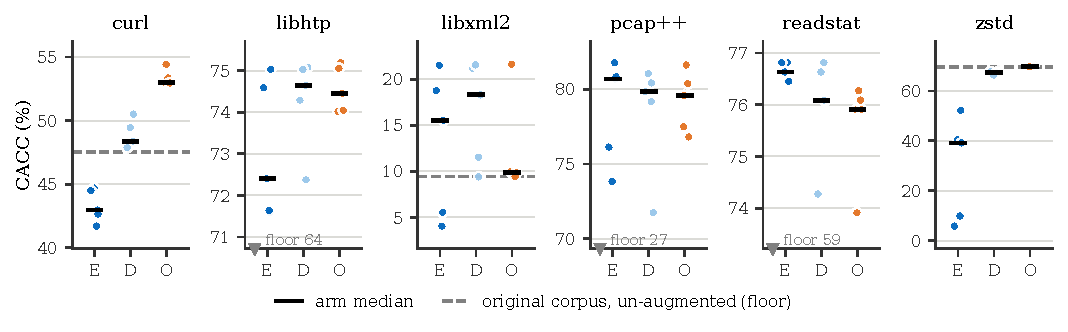
\includegraphics[width=\textwidth]{figures/rq1/corpus_coverage.pdf}
    \caption{\ac{CACC} of the final corpus across starting-corpus configurations}
    \label{fig:rq1:corpus_coverage}
\end{figure}

\paragraph{Affected-Code Coverage.}
The \ac{CACC} of the final corpus after the pipeline has run is depicted for each project under each starting-corpus configuration in \cref{fig:rq1:corpus_coverage}.
Across projects and arms, the median corpus improves on the un-augmented baseline, confirming that the agent contributes coverage of the affected code rather than merely preserving what the original corpus already reaches.
The exception is the \emph{empty} configuration, in which the agent must construct the entire corpus from scratch: on \texttt{curl} (\SI{-4.6}{\pp}) and \texttt{zstd} (\SI{-30.5}{\pp}) it does not recover the coverage that the original corpus provides for free.
The magnitude on \texttt{zstd} is the largest shortfall observed anywhere in the study, and it is accompanied by the widest within-arm spread, indicating that synthesizing valid inputs for this subject from nothing is both costly and unreliable.
Gains on \texttt{zstd} are slight in the other arms as well: starting from the \emph{original} corpus the agent adds only \SI[explicit-sign]{+0.3}{\pp}, and starting from the \emph{distilled} corpus it fails to recover what distillation discarded, ending \SI[explicit-sign]{-2.3}{\pp} below the baseline.
Distillation is therefore not uniformly reversible: reducing the corpus to a minimal covering set can remove structure that the agent cannot reconstruct within the trial budget.

The converse also holds, and more consistently: a complete starting corpus is not an advantage everywhere, and on \num{3} of the \num{6} subjects it is a liability.
On \texttt{readstat} and \texttt{pcap++} the \emph{empty} arm attains the highest median, marginally ahead of both other configurations, so the entire contribution of the supplied seeds is matched by an agent starting from nothing.
\texttt{libxml2} is the pronounced case: the \emph{original} arm finishes at a median of \SI{10.0}{\percent}, barely clearing the baseline of \SI{9.5}{\percent}, while \emph{distilled} reaches \SI{18.2}{\percent} and even \emph{empty} reaches \SI{15.5}{\percent} from no seeds at all.
Handing the agent the full corpus here leaves it close to where it started, whereas removing all but the seeds that touch the affected code nearly doubles the final coverage.
The pattern suggests that a large corpus occupies the agent's context with seeds that are irrelevant to the change site and anchors its synthesis to what those seeds already exercise, an effect that the distilled configuration avoids by construction and that the empty configuration cannot suffer from at all.

These per-project differences do not add up to a separation between arms.
The per-project tests in the \ac{CACC} block of \cref{tab:seeding-dimensions}, where arms are reported as scores normalized per project, resolve a pair on only two subjects, \texttt{curl} and \texttt{zstd}, in both cases \emph{original} over \emph{empty}; the remaining four yield no significant pair, with \texttt{libxml2} and \texttt{pcap++} at $p_{Holm} = \num{1.000}$ despite the spread visible in \cref{fig:rq1:corpus_coverage}.
Across all \num{6} projects the arms are indistinguishable ($p_{Holm} = \num{0.740}$), with \emph{empty} and \emph{original} tied at mean rank \num{2.17} and \emph{distilled} only slightly ahead at \num{1.67}.
No arm significantly outperforms both others on this criterion, so by the decision rule of \cref{sec:eval:seedgen:procedure} selection passes to corpus size.

\paragraph{Corpus Size and Composition.}
The composition of the final corpus is depicted in \cref{fig:rq1:corpus_size}, separating the seeds inherited from the starting corpus from those the agent generated during augmentation.
The generated component is strikingly insensitive to the configuration it starts from: on every subject and in every arm, it falls between roughly \numrange{100}{1000} seeds, and within a subject, the three arms generate counts of the same order.
The agent, therefore, produces an almost fixed volume of output per trial, governed by the cycle and cost budget rather than by what it was given, and the differences in final corpus size between arms are almost entirely inherited rather than earned.

\begin{figure}
    \centering
    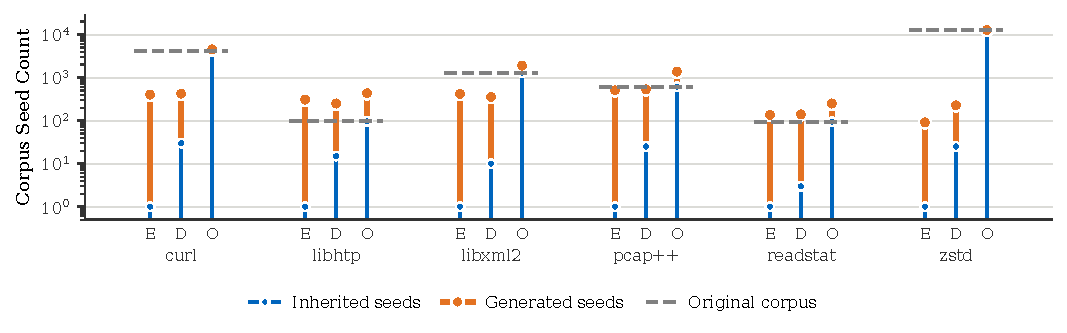
\includegraphics[width=\textwidth]{figures/rq1/corpus_size.pdf}
    \caption{Seed count of the final corpus across starting-corpus configurations}
    \label{fig:rq1:corpus_size}
\end{figure}

What separates the arms is consequently how much of the original corpus survives into the final one.
Distillation reduces the starting corpus by one to three orders of magnitude, most sharply on the seed-rich subjects: \texttt{zstd} falls from roughly \num{12000} seeds to \num{25}, \texttt{curl} from \num{4000} to \num{28}, and \texttt{libxml2} from \num{1300} to \num{10}.
Because the generated component is of fixed order, the \emph{distilled} arm ends within the same order of magnitude as \emph{empty} on every subject, whereas \emph{original} carries its full corpus through and ends an order of magnitude or more above both.
The extreme is \texttt{zstd}, where the \emph{original} arm finishes at roughly \num{12000} seeds against \num{230} for \emph{distilled}.

Read against \cref{fig:rq1:corpus_coverage}, this is where the \emph{original} configuration is least defensible.
On \texttt{zstd} its \num{12000} seeds buy \SI[explicit-sign]{+0.3}{\pp} over the un-augmented baseline, and on \texttt{libxml2} its \num{1900} seeds reach a median \ac{CACC} of \SI{10.0}{\percent} where the \emph{distilled} arm reaches \SI{18.2}{\percent} with roughly a fifth as many.
The seeds inherited from a complete corpus thus enlarge the fuzzer's search space without proportionately increasing coverage of the affected code.

Unlike the coverage criterion, this one separates the arms.
The corpus-size block of \cref{tab:seeding-dimensions} resolves a pair on \num{5} of the \num{6} subjects, always against \emph{original}: \emph{empty} and \emph{distilled} jointly on \texttt{curl}, \texttt{libxml2} and \texttt{pcap++}, \emph{distilled} alone on \texttt{libhtp} and \emph{empty} alone on \texttt{zstd}.
Only \texttt{readstat} resolves no pair after Holm correction despite a significant omnibus test ($p_{Holm} = \num{0.018}$).
Across all \num{6} projects the arms differ significantly ($p_{Holm} = \num{0.006}$), with \emph{original} ranked last on every subject without exception (mean rank \num{3.00}) and \emph{empty} narrowly ahead of \emph{distilled} at \num{1.33} against \num{1.67}.
The resolved pair, however, is \emph{empty} over \emph{original} alone: \emph{empty} and \emph{distilled} are not distinguishable from one another, so again no arm significantly outperforms both others, and selection passes to the normalized score.

\paragraph{Normalized Scoring of Starting Corpora.}
With neither criterion resolving the comparison, selection falls to the normalized scores in the \emph{All projects} row of \cref{tab:seeding-dimensions}.
The \emph{distilled} configuration leads on coverage (\num{98} against \num{92} for \emph{original} and \num{86} for \emph{empty}) while retaining a near-best corpus size (\num{88} against \num{94} for \emph{empty}), and is the only arm that is not ranked last on either criterion: \emph{empty} trails on coverage and \emph{original} collapses to \num{30} on corpus size.
It is therefore selected, though as a preference under a tie rather than an established difference, since neither criterion produced an arm that significantly outperformed both others.
The choice is not free: distillation requires preprocessing the original corpus before augmentation begins, an overhead that the \emph{empty} and \emph{original} configurations do not incur.
However, since the highest observed overhead is at most \SI{110}{\second} (\texttt{curl}), it is deemed negligible.

\begin{table}
  \centering
  \def\rk#1{\,\textsuperscript{(#1)}}%
  \def\hd#1{\multicolumn{5}{c}{#1}}%
  \begin{threeparttable}
    \footnotesize
    \setlength{\tabcolsep}{3pt}
    \begin{tabular*}{\textwidth}{@{\extracolsep{\fill}}l ccc S[table-format=1.3] l ccc S[table-format=1.3] l@{}}
       & \hd{(1) CACC ($\uparrow$)} & \hd{(2) Corpus size ($\downarrow$)} \\
      \cmidrule(lr){2-6}\cmidrule(lr){7-11}
      \textbf{Project} & \textbf{E} & \textbf{D} & \textbf{O} & {\textbf{$p_{Holm}$}} & \textbf{Pairs} & \textbf{E} & \textbf{D} & \textbf{O} & {\textbf{$p_{Holm}$}} & \textbf{Pairs} \\
      \midrule
      curl & 0.81\rk{3} & 0.91\rk{2} & \textbf{1.00}\rk{1} & {\textbf{$<$0.001}} & O\,$>$\,E & \textbf{1.00}\rk{1} & 0.95\rk{2} & 0.09\rk{3} & {\textbf{0.006}} & E,D\,$>$\,O \\
      libhtp & 0.97\rk{3} & \textbf{1.00}\rk{1} & 1.00\rk{2} & 0.969 & --- & 0.81\rk{2} & \textbf{1.00}\rk{1} & 0.58\rk{3} & {\textbf{0.003}} & D\,$>$\,O \\
      libxml2 & 0.85\rk{2} & \textbf{1.00}\rk{1} & 0.54\rk{3} & 1.000 & --- & 0.85\rk{2} & \textbf{1.00}\rk{1} & 0.19\rk{3} & {\textbf{0.005}} & E,D\,$>$\,O \\
      pcap++ & \textbf{1.00}\rk{1} & 0.99\rk{2} & 0.99\rk{3} & 1.000 & --- & \textbf{1.00}\rk{1} & 0.95\rk{2} & 0.37\rk{3} & {\textbf{0.006}} & E,D\,$>$\,O \\
      readstat & \textbf{1.00}\rk{1} & 0.99\rk{2} & 0.99\rk{3} & 0.097 & --- & \textbf{1.00}\rk{1} & 0.98\rk{2} & 0.54\rk{3} & {\textbf{0.018}} & --- \\
      zstd & 0.56\rk{3} & 0.96\rk{2} & \textbf{1.00}\rk{1} & {\textbf{$<$0.001}} & O\,$>$\,E & \textbf{1.00}\rk{1} & 0.40\rk{2} & 0.01\rk{3} & {\textbf{0.001}} & E\,$>$\,O \\
      \midrule
      \textbf{All projects} & 0.86\rk{2.17} & \textbf{0.98}\rk{1.67} & 0.92\rk{2.17} & 0.740 & --- & \textbf{0.94}\rk{1.33} & 0.88\rk{1.67} & 0.30\rk{3.00} & {\textbf{0.006}} & E\,$>$\,O \\
      \bottomrule
    \end{tabular*}
    \caption{Scoring of the starting corpus effectiveness}\label{tab:seeding-dimensions}
  \end{threeparttable}
\end{table}

\begin{tcolorbox}[colback=black!4, colframe=black!40, boxrule=0.4pt,left=6pt, right=6pt, top=6pt, bottom=6pt]
\paragraph{\textbf{\rqref{1.2}}}
The pipeline should be configured with the \emph{full} \ac{CoI} scope: although bounding the \ac{CoI} shrinks the target region by roughly an order of magnitude ($\Mdn \approx \num{9.7}\times$, range $\numrange{1.7}{66}\times$), the crash site falls outside the bounded target scope in \num{2} of \num{6} projects (\texttt{zstd}, \texttt{readstat}) and trades only a marginal, non-significant gain in bounded-scope coverage ($\dMdn = \SI[explicit-sign]{+1.3}{\pp}$, $p=\num{0.375}$) for a significant large loss in full-scope coverage ($\dMdn = \SI[explicit-sign]{-9.7}{\pp}$, $p=\num{0.031}$).
\end{tcolorbox}

\begin{figure}
    \centering
    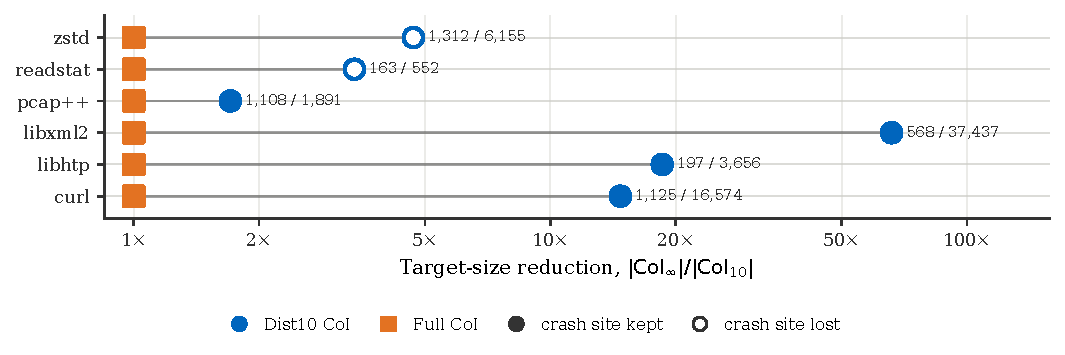
\includegraphics[width=\textwidth]{figures/rq1/coi-target-recall.pdf}
    \caption{Target size reduction and crash-site recall differences: Dist10-CoI vs. Full-CoI.}
    \label{fig:target_size_reduction}
\end{figure}

\paragraph{Target Area Size and Crash-Site Recall.}
The target size reduction and crash-site differences resulting from the distance-bounding ($\mathrm{CoI}_{10}$) policy are depicted in \cref{fig:target_size_reduction}.
Each project is presented separately with its reduction factor, the corresponding reduction in target lines of code, and whether the regression crash site is retained (filled circle) or excluded (hollow circle) by distance bounding.

Two main observations emerge.
First, the scale of target reduction depends heavily on the subject.
The observed reduction factors span from $\num{1.7}\times$ on \texttt{pcap++} up to $\num{66}\times$ on \texttt{libxml2}.
Across all subjects, bounding achieves a median target area reduction of $\num{9.7}\times$.
Thus, restricting the \ac{CoI} to a distance of \num{10} basic blocks from the change site yields orders-of-magnitude reductions in target static code size for most projects.
Second, this spatial reduction directly compromises defect safety.
For two targets, \texttt{zstd} and \texttt{readstat}, bounding the scope excludes the actual crash-site lines of the introduced regressions from the target set.
For these subjects, any coverage the pipeline achieves on the crash site is an indirect side effect of traversing the bounded region rather than a targeted objective.

\begin{figure}
    \centering
    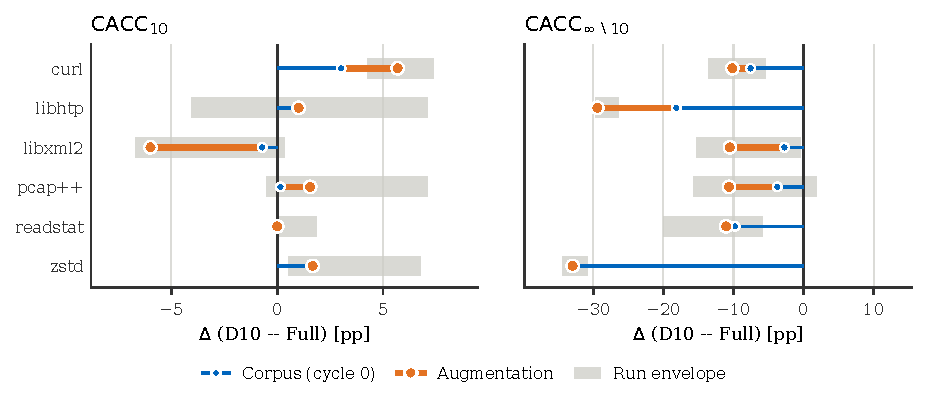
\includegraphics[width=\textwidth]{figures/rq1/cone-region-deltas.pdf}
    \caption{Median difference in \ac{CACC}: Dist10-CoI vs. Full-CoI}
    \label{fig:median_diff_coi_bound}
\end{figure}

\paragraph{Bounded and Complement Coverage.}
A reduced target scope is intended to focus the pipeline's synthesis effort, increasing coverage within the retained bounded region more effectively than an unbounded scope would.
The bounded ($\mathrm{CoI}_{10}$) and unbounded (Full) configurations, however, diverge at two stages: distillation already selects a different initial corpus (cycle~0), and the agent then pursues a different coverage target during augmentation.
\Cref{fig:median_diff_coi_bound} therefore splits the median difference for the near-change region ($\mathrm{CACC}_{10}$) and the complementary distant region ($\mathrm{CACC}_{\infty \setminus 10}$) into the part already present in the distilled corpus and the part added by augmentation.
\Cref{tab:coi_scope_score} details the statistical test results for the final corpora.

The bounded configuration yields a corpus that is markedly more concentrated in the near-change region.
Its distant coverage is lower across all projects, and the pooled difference is significant.
In \num{5} of the \num{6} projects, the separation is complete, with every bounded run ending below every unbounded run.
Only \texttt{pcap++} narrowly misses the significance threshold, because a single unbounded run ends level with the bounded median.
Much of this drop, however, stems from distillation rather than from the agent.
For \texttt{curl}, \texttt{libhtp}, \texttt{readstat}, and \texttt{zstd}, most of the gap is already present at cycle~0, and for \texttt{zstd} augmentation leaves it essentially unchanged.
Augmentation is the dominant contributor only for \texttt{libxml2} and \texttt{pcap++}.
For \texttt{curl}, \texttt{libhtp}, \texttt{libxml2}, and \texttt{zstd}, the bounded agent adds little distant coverage beyond its distilled corpus, whereas the unbounded agent continues to extend it.
For \texttt{pcap++} and \texttt{readstat}, in contrast, the bounded agent gains substantial distant coverage, nearly as much as the unbounded agent.
This suggests that inputs reaching the near-change code in these projects indirectly exercise large parts of the distant code.
Overall, the agent largely respects the boundary of its assigned target, but the magnitude of the drop is primarily due to the reduced initial corpus rather than to the agent's synthesis behavior.

Restricting the target scope, in contrast, yields negligible benefit within the bounded region itself.
The pooled gain in near-change coverage is small and not significant.
Separating the two stages shows that even this small gain is rarely attributable to more focused synthesis.
For \texttt{libhtp} and \texttt{zstd}, the entire difference is attributed to the distillation step, and both agents subsequently raise near-change coverage by the same amount.
The significant gain for \texttt{zstd}, therefore, originates from distillation, not from augmentation.
\texttt{readstat} shows no difference at either stage.
\texttt{pcap++} starts from nearly equivalent corpora, and both agents raise near-change coverage by similarly large amounts, leaving a small, non-significant difference.
Only \texttt{curl} exhibits a significant gain to which augmentation contributes meaningfully.
Roughly half of this gain is inherited from distillation, and the bounded agent adds the rest by extending its distilled corpus further than the unbounded agent does.
\texttt{libxml2} reverses the expected pattern.
Its distilled corpora are nearly equivalent, yet the bounded agent adds almost no near-change coverage, while the unbounded agent raises it substantially in several runs.
A possible explanation is that this near-change code is reachable via input structures that the bounded target does not incentivize.
For \texttt{libhtp}, \texttt{libxml2}, and \texttt{pcap++}, the per-run differences additionally span zero, indicating that run-to-run variation is of the same order as the observed effect.

\begin{table}
  \centering
  \def\rk#1{\,\textsuperscript{(#1)}}%
  \def\hd#1{\multicolumn{5}{c}{#1}}%
  \begin{threeparttable}
    \footnotesize
    \setlength{\tabcolsep}{3pt}
    \begin{tabular*}{\textwidth}{@{\extracolsep{\fill}}l cc c S[table-format=1.3] l cc c S[table-format=1.3] l@{}}
       & \hd{(1) $\mathrm{CACC}_{10}$ ($\uparrow$)} & \hd{(2) $\mathrm{CACC}_{\infty \setminus 10}$ ($\uparrow$)} \\
      \cmidrule(lr){2-6}\cmidrule(lr){7-11}
      \textbf{Project} & \textbf{CoI10} & \textbf{Full} & \textbf{$\Delta$} & {\textbf{$p_{Holm}$}} & {\textbf{$\hat A_{12}$}} & \textbf{CoI10} & \textbf{Full} & \textbf{$\Delta$} & {\textbf{$p_{Holm}$}} & {\textbf{$\hat A_{12}$}} \\
      \midrule
      curl & \textbf{74.7}\rk{1} & 69.0\rk{2} & $+$5.7 & {\textbf{0.048}} & 1.00 & 36.4\rk{2} & \textbf{46.6}\rk{1} & $-$10.2 & {\textbf{0.048}} & 0.00 \\
      libhtp & \textbf{93.9}\rk{1} & 92.9\rk{2} & $+$1.0 & 0.190 & 0.82 & 44.2\rk{2} & \textbf{73.6}\rk{1} & $-$29.4 & {\textbf{0.048}} & 0.00 \\
      libxml2 & 43.3\rk{2} & \textbf{49.3}\rk{1} & $-$6.0 & 0.063 & 0.04 & 7.3\rk{2} & \textbf{17.8}\rk{1} & $-$10.5 & {\textbf{0.048}} & 0.00 \\
      pcap++ & \textbf{85.6}\rk{1} & 84.1\rk{2} & $+$1.6 & 0.167 & 0.88 & 62.2\rk{2} & \textbf{72.8}\rk{1} & $-$10.6 & 0.056 & 0.12 \\
      readstat & \textbf{84.0}\rk{1} & \textbf{84.0}\rk{1} & $+$0.0 & 1.000 & 0.60 & 61.7\rk{2} & \textbf{72.8}\rk{1} & $-$11.1 & {\textbf{0.048}} & 0.00 \\
      zstd & \textbf{80.1}\rk{1} & 78.4\rk{2} & $+$1.7 & {\textbf{0.048}} & 1.00 & 31.0\rk{2} & \textbf{63.9}\rk{1} & $-$33.0 & {\textbf{0.048}} & 0.00 \\
      \midrule
      \textbf{All projects} & \textbf{82.1}\rk{1.17} & 81.2\rk{1.67} & $+$1.0 & 0.625 & 4W 1T 1L & 40.3\rk{2.00} & \textbf{68.3}\rk{1.00} & $-$19.8 & {\textbf{0.031}} & 0W 0T 6L \\
      \bottomrule
    \end{tabular*}
    \caption{Scoring of \ac{CoI} scoping effectiveness}
    \label{tab:coi_scope_score}
  \end{threeparttable}
\end{table}

\paragraph{\ac{CoI} Scope Decision.}
Overall, while the bounded configuration concentrates coverage within the local neighborhood of the change site, it fails to meaningfully improve coverage in that local region compared with an unbounded scope.
Simultaneously, it penalizes safety by excluding known regression crash sites and severely reducing coverage across the surrounding context.
Following the decision rule, the \emph{full} \ac{CoI} scope is selected for the pipeline to preserve safety and complement coverage without sacrificing local reachability.

\subsection{Discussion}
The findings from both seed augmentation studies highlight key trade-offs in configuring the augmentation pipeline.

\paragraph{Starting Corpus Composition.}
Supplying more seeds to the agent does not monotonically improve LLM-guided seed generation.
Even when starting from an empty reference corpus, the agent closely matches the change-affected code coverage of the resulting corpora, relying solely on inference over code semantics.
However, when a project already maintains a well-engineered corpus, as is the case for \texttt{curl} and \texttt{zstd}, the agent cannot match the value embedded in these hand-crafted inputs without access to them.
This underlines the value of building upon existing corpus knowledge whenever it is available.
Distillation offers an effective middle ground: it reduces the often massive original base corpora to a manageable set while still yielding improvements over that initial set.
The cost of this reduction is that coverage-based distillation cannot judge structural diversity and therefore discards information the agent could otherwise build upon.
This effect is visible for \texttt{curl}, where the final coverage achieved when starting from the original corpus exceeded that of the distilled starting corpus.
Inputs that do not reach the change region may nonetheless be structurally close to relevant ones, and thus serve as valuable templates from which the agent can derive change-targeted seeds.

\paragraph{Static Target Granularity vs.\ Semantic Relevance.}
% TODO: Finalize once the decomposition of distillation vs. LLM contribution is available.
Constraining the static target scope sharpens the focus of LLM-guided synthesis, but spatial concentration does not translate directly into higher coverage within the targeted region.
Distillation is an effective tool for making seeds more targeted, as it selects only those seeds that reach the target area.
More critically, restricting the static scope based purely on basic-block distance risks truncating control-flow paths that contain the true root causes or crash locations of regressions.
The distance threshold in the CoI-Fuzzer tool could be increased, but doing so defeats the purpose of bounding the scope in the first place.
While further truncation policies are implemented, none of them achieves a substantial reduction in scope while maintaining adequate safety.
Further research to define a safe subset of the full \ac{CoI} would therefore be valuable and further improve the presented pipeline.

\paragraph{Practical Pipeline Configuration.}
Together, these results reveal an asymmetric design principle for change-targeted seed generation: pipelines should be selective about the seeds supplied to the LLM, but conservative about the code scope considered relevant to the change.
Restricting the seed corpus via distillation reduces noise and context bloat during synthesis, while maintaining the full \ac{CoI} scope ensures that potential defect sites remain visible.
Consequently, carrying the \emph{distilled} starting corpus alongside the \emph{full} \ac{CoI} scope into end-to-end fuzzing campaigns provides the most effective baseline for downstream vulnerability discovery.

\section{Fuzzing Study}\label{sec:eval:fuzzing}
The second study evaluates the resulting corpus in an end-to-end fuzzing campaign, comparing the LLM-augmented corpus produced by the configuration selected in \rqref{1.1} and \rqref{1.2} against the project's original corpus.
It addresses the following research questions:

\begin{description}
  \item[\researchq{2.1} (reliability)] How often do campaigns seeded with each corpus expose the target regression bug within the campaign budget, with and without accounting for seed augmentation overhead??
  \item[\researchq{2.2} (generalization)] Does the detection rate on the subjects used to select the configuration differ from that on the held-out subjects?
  \item[\researchq{2.3} (efficiency)] How does the expected time-to-exposure of the target bug within the campaign budget differ between the two seed corpora, with and without accounting for seed augmentation overhead?
  \item[\researchq{2.4} (attribution)] What factors in the seed augmentation pipeline account for differences in regression exposure between campaigns using the augmented corpus and the baseline corpus?
\end{description}

Together, the research questions establish whether the gains observed in the seed generation study translate to an end-to-end fuzzing campaign and whether they hold for subjects who played no part in selecting the configuration.

\subsection{Subjects}\label{sec:eval:fuzzing:subjects}
This study uses all \num{12} subjects introduced in \autoref{sec:eval:subjects}.
\num{6} subjects were used to select the configuration in \autoref{sec:eval:seedgen}; the remaining \num{6} played no part in that selection and serve to expose any overfitting of the configuration to the selection set.
This split is marked in every per-subject table and plot, so that it remains visible whether an observed effect is confined to the subjects that informed the configuration.

Aggregate figures and statistical tests are computed over the full set of \num{12}; the split is not treated as a factor.
On \num{4} of the \num{6} held-out subjects, neither corpus exposed the bug within the budget, leaving too few informative subjects for a separate comparison.

\subsection{Procedure}\label{sec:eval:fuzzing:procedure}
Each subject is fuzzed under two arms: seeded with the project's original corpus, and seeded with the LLM-augmented corpus produced by the configuration selected in \autoref{sec:eval:seedgen}.
Corpus augmentation is performed once per subject, so the only source of randomness within an arm is the fuzzing campaign itself.
For the tuning set, the latest result from the \num{5} runs is evaluated in \cref{sec:eval:seedgen} to save costs, whereas for the held-out set, a single augmentation run was performed independently.
Costs are reported in \cref{tab:termination-fuzzing} but not evaluated within the scope of this study.

The campaign budget is \SI{8}{\hour}, the longest campaign that still fits an overnight CI/CD run~\cite{kloosterEffectivenessScalabilityFuzzing2022}.
This is shorter than the \SI{24}{\hour} convention common in fuzzer evaluations~\cite{klees2018}, and the trade-off runs in a direction that favors the technique under test: a short budget rewards seeds that pay off early, which is precisely what per-commit regression-targeted corpus augmentation is designed to produce.
This is stated explicitly rather than treating \SI{8}{\hour} as neutral, and revisited in \autoref{sec:eval:threats}.

Every arm is run for \num{10} independent campaigns per subject, each with a distinct fuzzer seed and no state shared between runs.
A campaign counts as a reproduction only when the crash matches the target regression: BugOSS supplies the bug-revealing input along with the bug, and a match is confirmed manually against the sanitizer report and the faulting location, rather than counting arbitrary crashes by matching the top frames of the call stack and their line numbers.

\paragraph{Unit of analysis.}
Campaigns are not pooled across subjects.
Corpus construction is performed once per subject, so the \num{10} campaigns within a subject are repeated measurements of one constructed corpus rather than independent samples of the technique, and the subject is the unit of analysis for every cross-subject statement.
Within a subject, the \num{10} campaigns are independent and are compared directly.

\paragraph{Time to Error.}
Campaigns that reach the budget without reproducing the bug have no \ac{TTE}.
These are treated as right-censored at \SI{8}{\hour} rather than discarded or imputed, following Magma~\cite{hazimehMagmaGroundTruthFuzzing2020}.
Each subject and arm is summarized by the \ac{RMST} at the \SI{8}{\hour} horizon: the average time for which the bug survives undetected over a campaign capped at \SI{8}{\hour}, computed as the area under the Kaplan--Meier estimate.
\ac{RMST} is defined for every subject, including those where fewer than half the campaigns reproduce the bug, and the median \ac{TTE} does not exist.
All reported \ac{RMST} values are relative to the \SI{8}{\hour} budget and are not comparable to figures obtained under a different horizon.
Statistical comparisons follow the continuous-outcome procedure for two arms in \autoref{sec:eval:statistics}.

\paragraph{Reproduction Rate.}
\ac{RMST} is the primary outcome of this study; the reproduction rate is the endpoint of the same survival curve and is reported as a reliability view of it, rather than as stand-alone evidence.
Reproduction rates are reported per subject as the fraction of campaigns exposing the bug, together with the mean rate per arm; statistical comparisons follow the binary-outcome procedure for two arms in \autoref{sec:eval:statistics}.

\paragraph{Case Attribution.}
\rqref{2.4} is answered by a post-hoc case attribution analysis in two steps: case selection, then tracing where the regression-exposing inputs came from.

First, the subjects that show suggestive evidence of a difference in \ac{RMST} between the arms, in either direction, are selected.
With only \num{10} campaigns per arm, the conventional threshold of $p < \num{0.05}$ would discard differences that are large but uncertain.
For selection, the threshold is therefore raised to $p_{Holm} < \num{0.15}$.
This is a filter for which subjects to explain, not a significance claim.
It excludes the \num{4} subjects without any exposure and the \num{3} subjects whose difference is indistinguishable from noise (\emph{libhtp}, \emph{readstat}, \emph{openssl}).
\num{5} subjects remain: \emph{yara}, \emph{pcap++}, \emph{libxml2}, \emph{zstd}, and \emph{curl}, of which only \emph{pcap++} is not significant at \num{0.05}.

Second, the provenance of the regression-exposing inputs is traced.
For every campaign, the \emph{first} crash that matches the target regression is taken.
As with \ac{RMST}, crashes after the \SI{8}{\hour} horizon do not count.
AFL++ records, for each queue entry, the entry it was mutated from.
These links are followed back to the corpus file the crash descends from, termed its \emph{ancestor}, and the number of queue entries on the way is termed its number of \emph{generations}.
Each unique ancestor is then located in the corpus stages of the pipeline (\cref{tab:attribution}):
\begin{description}
  \item[Baseline ancestors] unique ancestors of the original arm, over the
    size of the original corpus;
  \item[Distilled] unique ancestors of the augmented arm that were already
    in the distilled corpus, over its size;
  \item[Generated] unique ancestors of the augmented arm that entered the
    corpus after distillation, over the number of files added after it.
  \item[Final corpus] the union of both, over the size of the corpus, the augmented fuzzing campaigns were seeded with.
\end{description}
\emph{Crash} marks an arm whose corpus already reproduced the regression during pre-fuzzing screening, so the campaigns never had to fuzz.
Each case is then read through its ancestors, the files themselves, where needed, and the generation counts.
Finally, the cases are grouped by which stage supplied the exposing input.
The attribution shows which seed a crash actually descends from.
It does not show that any other seed could have led to the crash.
It explains the observed difference, but it is not a counterfactual.

\subsection{Results}
\begin{figure}
  \centering
  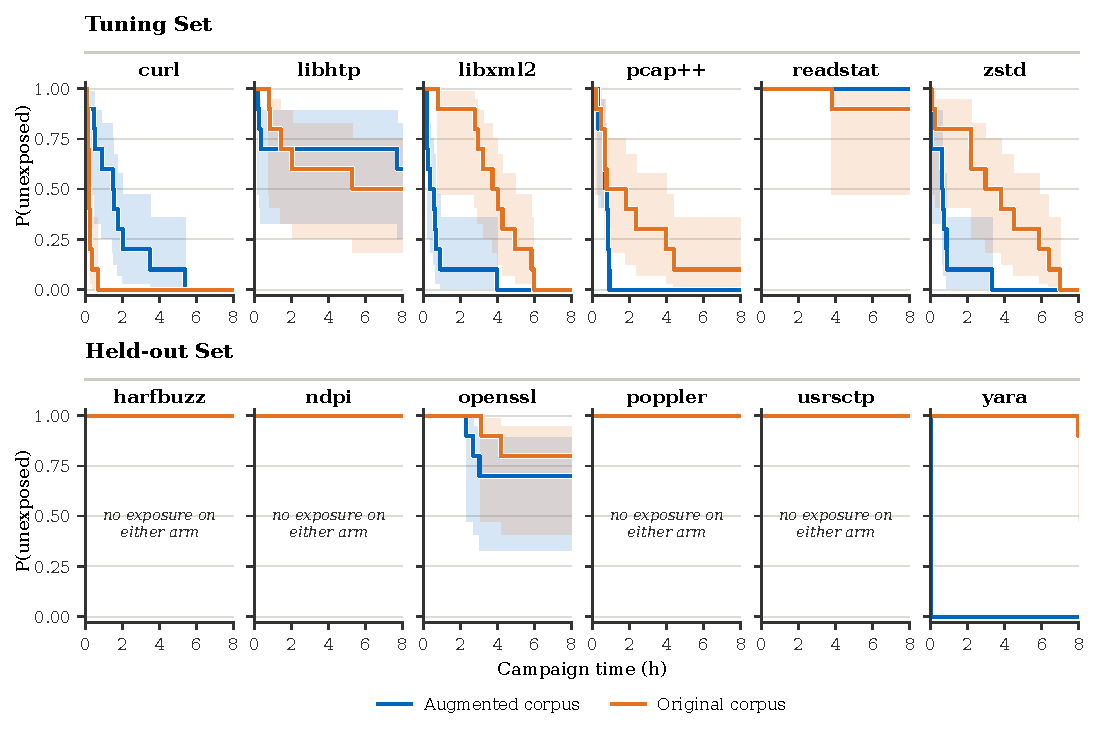
\includegraphics[width=\textwidth]{figures/bug-survival-curves.pdf}
  \caption[Bug Survival Curves]{%
    Kaplan--Meier estimate bug survival curves, one tile per project, with error bands.
  \label{fig:bug_survival_curves}
  }
\end{figure}

\Cref{fig:bug_survival_curves} summarizes the campaign outcomes as subject-level survival curves over the \SI{8}{\hour} horizon, one panel per subject with a separate curve per arm.
Higher curves mean the bug survived longer, and steep drops mark reproductions.
The \num{4} held-out subjects that yielded no exposure at all remain flat at \num{1.0} across the horizon, while \emph{yara}'s augmented arm starts at \num{0.0} because its corpus already contained a bug-exposing input before fuzzing began.
Numeric summaries derived from these curves are reported alongside each research question below.

\begin{table}
  \centering
  \def\rk#1{\,\textsuperscript{(#1)}}%
  \def\hd#1{\multicolumn{4}{c}{#1}}%
  \begin{threeparttable}
    \footnotesize
    \setlength{\tabcolsep}{3pt}
    \begin{tabular*}{\textwidth}{@{\extracolsep{\fill}}l cc c S[table-format=1.3] cc c S[table-format=1.3]@{}}
      \textbf{Reproduction rate ($\uparrow$)} & \hd{(1) Without overhead} & \hd{(2) With overhead} \\
      \cmidrule(lr){2-5}\cmidrule(lr){6-9}
      \textbf{Project} & \textbf{Augmented} & \textbf{Original} & \textbf{$\Delta$} & {\textbf{$p_{Holm}$}} & \textbf{Augmented} & \textbf{Original} & \textbf{$\Delta$} & {\textbf{$p_{Holm}$}} \\
      \midrule
      \addlinespace[2pt]
      \multicolumn{9}{@{}l}{\textsc{Tuning set}\ \textnormal{(6 projects)}} \\
      \addlinespace[1pt]
      \hspace{1em}curl & 1.00\rk{1} & 1.00\rk{1} & \phantom{$+$}0.00 & {--} & 1.00\rk{1} & 1.00\rk{1} & \phantom{$+$}0.00 & {--} \\
      \hspace{1em}libhtp & 0.40\rk{2} & \textbf{0.50}\rk{1} & $-$0.10 & 1.000 & 0.30\rk{2} & \textbf{0.50}\rk{1} & $-$0.20 & 1.000 \\
      \hspace{1em}libxml2 & 1.00\rk{1} & 1.00\rk{1} & \phantom{$+$}0.00 & {--} & 1.00\rk{1} & 1.00\rk{1} & \phantom{$+$}0.00 & {--} \\
      \hspace{1em}pcapplusplus & \textbf{1.00}\rk{1} & 0.90\rk{2} & $+$0.10 & 1.000 & \textbf{1.00}\rk{1} & 0.90\rk{2} & $+$0.10 & 1.000 \\
      \hspace{1em}readstat & 0.00\rk{2} & \textbf{0.10}\rk{1} & $-$0.10 & 1.000 & 0.00\rk{2} & \textbf{0.10}\rk{1} & $-$0.10 & 1.000 \\
      \hspace{1em}zstd & 1.00\rk{1} & 1.00\rk{1} & \phantom{$+$}0.00 & {--} & 1.00\rk{1} & 1.00\rk{1} & \phantom{$+$}0.00 & {--} \\
      \addlinespace[6pt]
      \multicolumn{9}{@{}l}{\textsc{Held-out set}\ \textnormal{(6 projects)}} \\
      \addlinespace[1pt]
      \hspace{1em}harfbuzz & 0.00\rk{1} & 0.00\rk{1} & \phantom{$+$}0.00 & {--} & 0.00\rk{1} & 0.00\rk{1} & \phantom{$+$}0.00 & {--} \\
      \hspace{1em}ndpi & 0.00\rk{1} & 0.00\rk{1} & \phantom{$+$}0.00 & {--} & 0.00\rk{1} & 0.00\rk{1} & \phantom{$+$}0.00 & {--} \\
      \hspace{1em}openssl & \textbf{0.30}\rk{1} & 0.20\rk{2} & $+$0.10 & 1.000 & \textbf{0.30}\rk{1} & 0.20\rk{2} & $+$0.10 & 1.000 \\
      \hspace{1em}poppler & 0.00\rk{1} & 0.00\rk{1} & \phantom{$+$}0.00 & {--} & 0.00\rk{1} & 0.00\rk{1} & \phantom{$+$}0.00 & {--} \\
      \hspace{1em}usrsctp & 0.00\rk{1} & 0.00\rk{1} & \phantom{$+$}0.00 & {--} & 0.00\rk{1} & 0.00\rk{1} & \phantom{$+$}0.00 & {--} \\
      \hspace{1em}yara & \textbf{1.00}\rk{1} & 0.10\rk{2} & $+$0.90 & {\textbf{$<$0.001}} & \textbf{1.00}\rk{1} & 0.10\rk{2} & $+$0.90 & {\textbf{$<$0.001}} \\
      \midrule
      \textbf{All projects} & \textbf{0.48}\rk{1.17} & 0.40\rk{1.25} & \phantom{$+$}0.00 & 1.000 & \textbf{0.47}\rk{1.17} & 0.40\rk{1.25} & \phantom{$+$}0.00 & 1.000 \\
      \bottomrule
    \end{tabular*}
    \caption{Fuzzing crash reproduction rate across subjects.}\label{tab:bugeval-reproduction}
  \end{threeparttable}
\end{table}


\begin{tcolorbox}[colback=black!4, colframe=black!40, boxrule=0.4pt,
                  left=6pt, right=6pt, top=6pt, bottom=6pt]
\rqref{2.1} Across the \num{12} subjects, the augmented corpus reproduced the regression more often in three, less often in two and equally often in seven (\SI{48}{\percent} vs.\ \SI{40}{\percent} of campaigns, \SI{47}{\percent} with the pipeline overhead charged), a median paired difference of zero that is not significant with or without the overhead ($p = \num{1.00}$).
\end{tcolorbox}


Per-subject reproduction rates are reported in \cref{tab:bugeval-reproduction}.
Only \emph{yara} separates the arms within a subject after Holm adjustment:
its augmented corpus exposed the bug in all \num{10} campaigns, against \num{1} of \num{10} for the original corpus.
The remaining differences are one-campaign-wide, and none are significant.

The seven tied subjects are tied for two opposite reasons, and the distinction matters for the rest of this section.
Four of them (\emph{harfbuzz}, \emph{ndpi}, \emph{poppler}, \emph{usrsctp}) produced no exposure in either arm, so the measure has nothing to separate.
The other three (\emph{curl}, \emph{libxml2}, \emph{zstd}) reproduced the bug in \emph{every} campaign of \emph{both} arms, so the reproduction rate is saturated at \num{1.00} and cannot express a difference that exists.
As \cref{tab:bugeval-rmst} shows, all three of these subjects separate clearly on time to exposure.
The reproduction rate is therefore reported here as a reliability view of the survival curve rather than as the efficiency measure, and \ac{RMST} is the primary outcome.

When accounting for the overhead introduced by the pipeline, only one exposure on \emph{libhtp} exceeded the adjusted \SI{8}{\hour} window, reducing its augmented reproduction rate from \num{0.40} to \num{0.30}.
All other rates are unchanged: every other augmented exposure still fell inside the window after its subject's overhead was added, which ranges from about \SI{45}{\minute} to \SI{2.75}{\hour} (\cref{tab:bugeval-rmst}).
The overhead, therefore, leaves the reproduction picture intact.
\emph{yara} remains the only subject that separates the arms, and the pooled sign test stays at $p = \num{1.000}$.

\begin{tcolorbox}[colback=black!4, colframe=black!40, boxrule=0.4pt,
                  left=6pt, right=6pt, top=6pt, bottom=6pt]
\rqref{2.2} Generalization to the held-out subjects remains inconclusive: on \num{4} of the \num{6} neither corpus exposed the bug within the budget, leaving \num{2} informative subjects, one of which reflects a corpus that already contained a bug-exposing input before fuzzing began.
\end{tcolorbox}

Of the \num{6} held-out subjects, \emph{harfbuzz}, \emph{ndpi}, \emph{poppler} and \emph{usrsctp} produced no reproduction in either arm across all \num{20} campaigns, so neither the reproduction rate nor the \ac{TTE} can distinguish the corpora there.
The two remaining subjects are \emph{yara} and \emph{openssl}.
\emph{Yara}'s effect is the largest in the study but does not measure fuzzing at all: the augmented corpus contained an input that crashed the target before the first campaign second, so the comparison records corpus construction rather than search.
Setting it aside leaves \emph{openssl}, whose advantage is \num{1} campaign in \num{10} and not significant.
No claim about generalization is supported in either direction by this evidence.

\begin{table}
  \centering
  \def\rk#1{\,\textsuperscript{(#1)}}%
  \def\hd#1{\multicolumn{4}{c}{#1}}%
  \begin{threeparttable}
    \footnotesize
    \setlength{\tabcolsep}{3pt}
    \begin{tabular*}{\textwidth}{@{\extracolsep{\fill}}l cc c S[table-format=1.3] cc c S[table-format=1.3]@{}}
      \textbf{$RMST_{8h}$ (h:mm) ($\downarrow$)} & \hd{(1) Without overhead} & \hd{(2) With overhead} \\
      \cmidrule(lr){2-5}\cmidrule(lr){6-9}
      \textbf{Project} & \textbf{Augmented} & \textbf{Original} & \textbf{$\Delta$} & {\textbf{$p_{Holm}$}} & \textbf{Augmented} & \textbf{Original} & \textbf{$\Delta$} & {\textbf{$p_{Holm}$}} \\
      \midrule
      \addlinespace[2pt]
      \multicolumn{9}{@{}l}{\textsc{Tuning set}\ \textnormal{(6 projects)}} \\
      \addlinespace[1pt]
      \hspace{1em}curl & 1:45\rk{2} & \textbf{0:14}\rk{1} & $+$1:30 & {\textbf{0.005}} & 2:51\rk{2} & \textbf{0:14}\rk{1} & $+$2:37 & {\textbf{$<$0.001}} \\
      \hspace{1em}libhtp & 5:38\rk{2} & \textbf{5:02}\rk{1} & $+$0:36 & 1.000 & 5:54\rk{2} & \textbf{5:02}\rk{1} & $+$0:51 & 1.000 \\
      \hspace{1em}libxml2 & \textbf{0:47}\rk{1} & 3:50\rk{2} & $-$3:02 & {\textbf{0.003}} & \textbf{2:08}\rk{1} & 3:50\rk{2} & $-$1:41 & 0.082 \\
      \hspace{1em}pcapplusplus & \textbf{0:41}\rk{1} & 2:19\rk{2} & $-$1:37 & 0.130 & \textbf{1:30}\rk{1} & 2:19\rk{2} & $-$0:48 & 1.000 \\
      \hspace{1em}readstat & 8:00\rk{2} & \textbf{7:34}\rk{1} & $+$0:25 & 1.000 & 8:00\rk{2} & \textbf{7:34}\rk{1} & $+$0:25 & 1.000 \\
      \hspace{1em}zstd & \textbf{0:46}\rk{1} & 3:30\rk{2} & $-$2:44 & {\textbf{0.020}} & \textbf{1:49}\rk{1} & 3:30\rk{2} & $-$1:41 & 0.281 \\
      \addlinespace[6pt]
      \multicolumn{9}{@{}l}{\textsc{Held-out set}\ \textnormal{(6 projects)}} \\
      \addlinespace[1pt]
      \hspace{1em}harfbuzz & 8:00\rk{1} & 8:00\rk{1} & \phantom{$+$}0:00 & {--} & 8:00\rk{1} & 8:00\rk{1} & \phantom{$+$}0:00 & {--} \\
      \hspace{1em}ndpi & 8:00\rk{1} & 8:00\rk{1} & \phantom{$+$}0:00 & {--} & 8:00\rk{1} & 8:00\rk{1} & \phantom{$+$}0:00 & {--} \\
      \hspace{1em}openssl & \textbf{6:23}\rk{1} & 7:07\rk{2} & $-$0:43 & 1.000 & 7:13\rk{2} & \textbf{7:07}\rk{1} & $+$0:05 & 1.000 \\
      \hspace{1em}poppler & 8:00\rk{1} & 8:00\rk{1} & \phantom{$+$}0:00 & {--} & 8:00\rk{1} & 8:00\rk{1} & \phantom{$+$}0:00 & {--} \\
      \hspace{1em}usrsctp & 8:00\rk{1} & 8:00\rk{1} & \phantom{$+$}0:00 & {--} & 8:00\rk{1} & 8:00\rk{1} & \phantom{$+$}0:00 & {--} \\
      \hspace{1em}yara & \textbf{0:00}\rk{1} & 7:59\rk{2} & $-$7:59 & {\textbf{$<$0.001}} & \textbf{0:56}\rk{1} & 7:59\rk{2} & $-$7:03 & {\textbf{$<$0.001}} \\
      \midrule
      \textbf{All projects} & \textbf{4:40}\rk{1.25} & 5:48\rk{1.42} & $-$1:11 & 0.148 & \textbf{5:11}\rk{1.33} & 5:48\rk{1.33} & $-$0:31 & 0.641 \\
      \bottomrule
    \end{tabular*}
    \caption{Fuzzing \ac{RMST} across subjects.}\label{tab:bugeval-rmst}
  \end{threeparttable}
\end{table}

\begin{tcolorbox}[colback=black!4, colframe=black!40, boxrule=0.4pt,
                  left=6pt, right=6pt, top=6pt, bottom=6pt]
\rqref{2.3} Across the \num{12} subjects, the augmented corpus reduced \ac{RMST} in \num{5}, increased it in \num{3}, and left it unchanged in \num{4}, with a median paired difference of \SI{71}{\minute} during fuzzing execution and \SI{31}{\minute} once the augmentation overhead is charged to each campaign (neither significant, $p = \num{0.148}$ and $p = \num{0.641}$).
\end{tcolorbox}

\Cref{tab:bugeval-rmst} reports \ac{RMST} per subject and arm.
\num{4} subjects separate after Holm adjustment.
Three favor augmentation (\texttt{yara}, \texttt{libxml2}, and \texttt{zstd}) and one favors the original corpus: \texttt{curl} exposed the bug \SI{1}{\hour}\,\SI{31}{\minute} later under augmentation.
Of the remaining subjects, \texttt{pcap++} and \texttt{openssl} favor augmentation, and \emph{libhtp} and \emph{readstat} the original, none significantly, and \num{4} admit no test because neither arm ever exposed the bug.

\begin{figure}
  \centering
  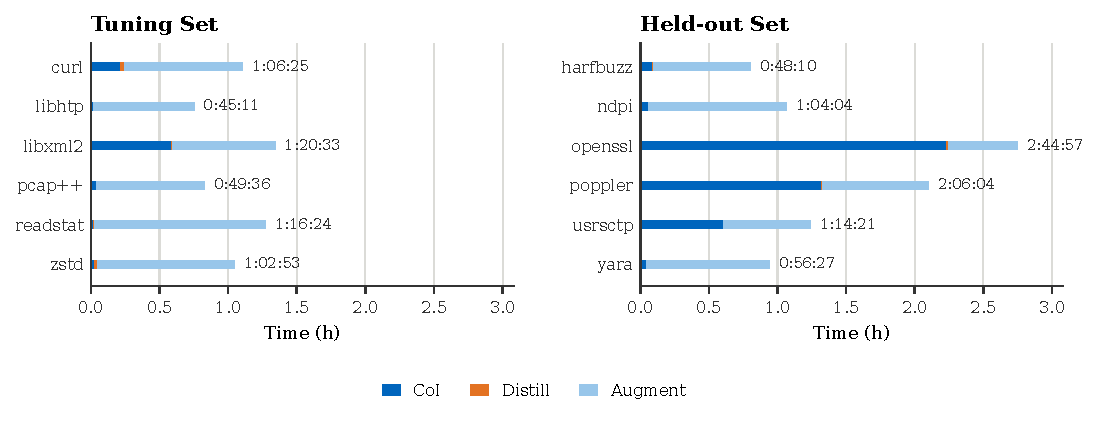
\includegraphics[width=\textwidth]{figures/augmentation-overhead.pdf}
  \caption{Time overhead of TACCO's augmentation stage}
  \label{fig:aug_overhead}
\end{figure}

Charging every augmented campaign with the wall-clock cost of the augmentation pipeline (\cref{fig:aug_overhead}) before applying the horizon shifts the split from five--four--three to four--four--four and shrinks the median paired difference from \SI{71}{\minute} to \SI{31}{\minute}, at which point the difference is no longer significant ($p = \num{0.641}$).
The overhead comes mainly from two phases.
The \ac{LLM} agent augmentation phase has a fairly consistent duration across projects, with a median of \SI{41}{\minute}.
The duration of the \ac{CoI} computation phase depends on project size, with a median of \SI{4.5}{\minute} and a range from \SI{1}{\minute} (\texttt{libhtp}) to \SI{134}{\minute} (\texttt{openssl}).
The overhead introduced by distillation is negligible in this context, with a maximum runtime of \SI{204}{\second} for \texttt{curl}.

\begin{tcolorbox}[colback=black!4, colframe=black!40, boxrule=0.4pt,
                  left=6pt, right=6pt, top=6pt, bottom=6pt]
\rqref{2.4} Exposure differences trace back to the pipeline's two stages, whose effects can reinforce or offset each other.
\begin{itemize}
  \item \textbf{Distillation} speeds up exposure by concentrating the budget on an ancestor that the original corpus already had (\emph{zstd}, \emph{libxml2}).
    It slows exposure by discarding the original corpus's close representatives of the required structure (\emph{curl}).
  \item \textbf{Generation} speeds up exposure when it supplies a structure the original corpus lacked entirely (\emph{yara}, \emph{pcap++}).
    It only partly compensates when it reconstructs what distillation dropped (\emph{curl}).
\end{itemize}
\end{tcolorbox}

\begin{table}
  \centering
  \begin{threeparttable}
    \footnotesize
    \setlength{\tabcolsep}{6pt}
    \sisetup{group-separator = {,}, group-minimum-digits = 4}
    \begin{tabular}{l l
                    S[table-format=5.0]
                    S[table-format=2.0]
                    S[table-format=3.0]
                    S[table-format=3.0]
                    r}
      \toprule
      \textbf{Project} & &  & \multicolumn{3}{c}{\textbf{Pipeline}} & \\
      \cmidrule(lr){4-6}
       & & {\textbf{Baseline}} & {\textbf{Distilled}} & {\textbf{Generated}} & {\textbf{Final corpus}} & \textbf{$\Delta$ RMST} \\
      \midrule
      \multirow{2}{*}{yara}    & \textit{unique ancestors} & 1     & 0  & 3   & \multicolumn{1}{c}{\multirow{2}{*}{\textit{Crash}}} & \multirow{2}{*}{$-$7:59:50} \\
                               & \textit{corpus size}      & 9     & 5  & 100 &     & \\
      \addlinespace
      \multirow{2}{*}{pcap++}  & \textit{unique ancestors} & 5     & 0  & 5   & 5   & \multirow{2}{*}{$-$1:37:50} \\
                               & \textit{corpus size}      & 615   & 25 & 505 & 530 & \\
      \addlinespace
      \multirow{2}{*}{libxml2} & \textit{unique ancestors} & 9     & 1  & 0   & 1   & \multirow{2}{*}{$-$3:02:25} \\
                               & \textit{corpus size}      & 1309  & 10 & 392 & 402 & \\
      \addlinespace
      \multirow{2}{*}{zstd}    & \textit{unique ancestors} & 5     & 1  & 0   & 1   & \multirow{2}{*}{$-$2:44:49} \\
                               & \textit{corpus size}      & 12462 & 25 & 91  & 116 & \\
      \addlinespace
      \multirow{2}{*}{curl}    & \textit{unique ancestors} & 8     & 1  & 7   & 8   & \multirow{2}{*}{$+$1:30:45} \\
                               & \textit{corpus size}      & 4202  & 30 & 478 & 508 & \\
      \bottomrule
    \end{tabular}
    \caption{Attribution results for the five selected subjects.}\label{tab:attribution}
  \end{threeparttable}
\end{table}

\Cref{tab:attribution} gives, for each selected subject, the corpus stage from which its exposing inputs descend.
The cases are discussed in the order of the attribution patterns they form.

\paragraph{pcap++.}
PcapPlusPlus is a C++ library for capturing and parsing network traffic; its fuzz target decodes each protocol layer of a packet capture (\texttt{.pcap} file).
The regression concerns the TLS \emph{CertificateRequest}, a handshake message in which a server asks for a client certificate.
Here, the pipeline's advantage comes from generation: the original corpus contains no TLS handshake at all, so no distillation could have preserved one.
All augmented campaigns descend from \num{5} agent-written captures, half of them from \texttt{ssl\_certreq\_clamp.pcap}.
This seed is a minimal, valid CertificateRequest with deliberately inconsistent content, announcing \num{255} certificate types in a message only \SI{2}{\byte} long.
From it, a single generation sufficed: every descending crash zeroes the low byte of the length field, and in one campaign that byte is the only difference between seed and crash.
The baseline campaigns reached the same crash from captures of unrelated protocols, but first spent \numrange{6}{18} generations building a valid TLS record.
As a result, the gain lies in reliability rather than typical speed.
Median time to exposure is almost equal, but all pipeline campaigns exposed the bug within \SI{55}{\minute}, whereas the slowest baseline campaign took \SI{4.4}{\hour}, and one never exposed it, which accounts for the difference in \ac{RMST}.
Distillation played no role: \num{4} of the \num{5} baseline ancestors survived it, yet no pipeline campaign descends from them, because the generated seeds were much closer to the crash.
This difference is attributed to generation.

\paragraph{yara.}
YARA is a pattern-matching tool used to classify malware; its PE module parses Windows executables (the Portable Executable format), and the regression lies in how it handles section names.
This is the most extreme case: the pipeline exposed the bug before fuzzing began.
During pre-fuzzing screening, \num{3} agent-written PE32 files, none of which were in the original corpus, had already reproduced it.
The original corpus, by contrast, led to the bug in only \num{1} of \num{10} campaigns, after \SI{7.97}{\hour} and \num{9} generations.
Distillation kept that test case, so the pipeline lost nothing, while generation added inputs that required no fuzzing at all; hence, $\Delta$~\ac{RMST} spans almost the entire horizon.
As noted for \rqref{2.2}, this case measures corpus construction rather than search.
This difference is attributed to generation.

\paragraph{libxml2.}
libxml2 is a widely used XML parser.
Here the pipeline did not bring the exposing input closer to the crash; it made that input far more likely to be fuzzed.
All augmented campaigns descend from one original seed, \texttt{ent\_738805.xml}, an XML document with entity declarations that distillation kept and that lies \numrange{2}{6} generations from the crash.
\num{9} of the pipeline campaigns exposed the bug within \SI{54}{\minute}.
In the baseline, the one campaign that descends from the same seed was just as fast (\SI{47}{\minute}, \num{3} generations).
The other \num{9} started from seeds that distillation dropped, needing up to \num{30} generations and a median of \SI{3.9}{\hour}.
The difference is in scheduling: after distillation, the exposed seed was \num{1} of \num{402} files rather than \num{1} of \num{1309}.
Generation contributed nothing, as none of the \num{392} \ac{LLM}-generated files are ancestors.
This difference is attributed to distillation.

\paragraph{zstd.}
zstd is a compression library implementing the Zstandard format; its fuzz target decompresses arbitrary input.
zstd shows the same mechanism as libxml2 more clearly: the bug is easy to reach from the original corpus, but the exposing seeds are buried in it.
The baseline had \num{5} ancestors, each only \numrange{1}{4} generations from the crash, yet needed a median of \SI{3.4}{\hour} (at most \SI{7.0}{\hour}), because AFL++ spreads its schedule over \num{12462} files.
Distillation dropped all \num{5} but kept a sixth original seed that is just as close.
All \num{10} pipeline campaigns descend from it within \numrange{1}{2} generations, with a median of \SI{39}{\minute}; \num{3} exposed the bug within the first minute.
Again, generation played no role: none of the \num{91} added files are ancestors, and the pipeline's ancestors are not closer to the crash (median \num{2} generations vs.\ \num{1}).
This difference is attributed to distillation.

\paragraph{curl.}
curl is a library and command-line tool for transferring data over protocols such as HTTP; its fuzz target replays scripted client--server exchanges.
curl is the only selected subject on which the pipeline was slower, because distillation removed the seeds closest to the bug and generation only partly replaced them.
The original corpus represents the exposing structure widely: all \num{10} baseline campaigns exposed the bug within \SI{41}{\minute} (median \SI{12}{\minute}), each \numrange{1}{2} generations from one of \num{8} distinct seeds.
Distillation dropped all \num{8}.
The one remaining original ancestor led a single pipeline campaign to the bug, after \num{4} generations and \SI{3.5}{\hour}.
The other \num{9} campaigns descend from \num{7} agent-written HTTP exchanges centered on redirects and authentication.
The agent thus aimed at the right functionality, but its seeds lie \numrange{1}{10} generations from the crash rather than \numrange{1}{2}, resulting in a median of \SI{1.5}{\hour} and a maximum of \SI{5.4}{\hour}.
This difference is attributed to distillation and is only partly offset by generation.

% ===================================================================
% (C) Results: synthesis
% ===================================================================

\paragraph{Synthesis.}
\Cref{tab:attribution-patterns} groups the five cases into three attribution patterns.

\begin{table}[t]
  \centering
  \begin{threeparttable}
    \footnotesize
    \begin{tabular}{p{0.24\linewidth} l p{0.20\linewidth} l l}
      \toprule
      \textbf{Pattern} & \textbf{Subjects} & \textbf{Augmented ancestors}
        & \textbf{Gens.\ to crash}\tnote{a} & \textbf{Exposure}\tnote{a} \\
      \midrule
      Distillation concentrates budget on an existing seed
        & \emph{zstd}, \emph{libxml2}
        & Distilled originals only
        & No closer
        & Faster \\
      \addlinespace
      Generation adds structure missing from the corpus
        & \emph{yara}, \emph{pcap++}
        & Agent-written only
        & \numrange{0}{2} vs.\ \numrange{6}{18}
        & Immediate to mixed \\
      \addlinespace
      Distillation drops exposing inputs; generation restores farther seeds
        & \emph{curl}
        & \num{9} of \num{10} generated; all \num{8} baseline ancestors discarded
        & \numrange{1}{10} vs.\ \numrange{1}{2}
        & Slower \\
      \bottomrule
    \end{tabular}
    \begin{tablenotes}
      \item[a] Augmented vs.\ baseline.
    \end{tablenotes}
    \caption{Attribution patterns across the cases in \cref{tab:attribution}.}
    \label{tab:attribution-patterns}
  \end{threeparttable}
\end{table}

The two stages of the pipeline act on different properties of the corpus.
Distillation does not change how close any seed is to the crash.
It changes how much of the campaign budget each seed receives.
This helps when a close ancestor survives (\emph{zstd}, \emph{libxml2}) and hurts when the close ancestors are the ones that get discarded (\emph{curl}).
Generation, by contrast, changes which structures exist in the corpus at all.
It pays off most when the original corpus has no input with the structure the regression requires, so that the baseline must first build that structure through mutation (\emph{pcap++}) or almost never builds it (\emph{yara}).
Where generation merely stands in for inputs that distillation removed, its seeds reach the regression, but from farther away than the originals did (\emph{curl}).

\subsection{Discussion}
 
\paragraph{Did the seed-generation gains translate?}
The largest coverage gain in the configuration study was on \texttt{libxml2}, where the \emph{distilled} arm nearly doubled \ac{CACC} over the baseline (\SI{18.2}{\percent} against \SI{9.5}{\percent}).
This subject also shows one of the largest \ac{RMST} reductions in the fuzzing study, but the attribution analysis shows that the reduction does not stem from the coverage the agent added: none of the \num{392} generated files is an ancestor of an exposing input, and every augmented campaign descends from a single distilled original seed.
The same holds for \texttt{zstd}, whose final \ac{CACC} under the \emph{distilled} configuration even ended slightly below the baseline, yet whose exposure time fell by more than two and a half hours.
Conversely, the subjects on which generation did supply the exposing input, \texttt{pcap++} and \texttt{yara}, did not stand out in the configuration study.
On \texttt{curl}, the configuration study already indicated that the \emph{original} corpus reached more affected code than the \emph{distilled} one, and the fuzzing study reproduces this ordering as the only significant slowdown.
Affected-code coverage of the corpus is therefore an imperfect proxy for regression exposure: it captures whether the change region is reached, but not whether a seed carries the specific structure the regression requires, nor how much of the fuzzing budget that seed receives.
 
\paragraph{When does augmentation help?}
The attribution cases suggest two distinct mechanisms, each tied to a property of the original corpus.
Generation pays off where the original corpus is small or lacks an input structure that the regression depends on.
\texttt{yara} starts from only \num{9} seeds covering \SI{20.7}{\percent} of the affected code, and none of the \num{615} captures of \texttt{pcap++} contains a TLS handshake.
What the agent contributed in these cases is of two kinds.
The first is format knowledge, such as a valid TLS handshake or a well-formed PE file; this is useful, but it is not specific to the \ac{LLM}, since public sample files or format-aware generators could supply the same structure.
The second is change-targeted content, such as the deliberately inconsistent CertificateRequest in \texttt{ssl\_certreq\_clamp.pcap}, which appears aimed at the changed length-handling logic and left the fuzzer a single generation from the crash.
Only this second kind is distinctly a contribution of the \ac{LLM}.
 
Distillation, in turn, pays off where the original corpus is large and the exposing seed already exists but is diluted among many others, as in \texttt{libxml2} (\num{1309} seeds) and \texttt{zstd} (\num{12462} seeds).
Concentrating the fuzzer's schedule on the few seeds that reach the affected code is then enough to reduce exposure time by hours, without any seed moving closer to the crash.
\texttt{curl} is the counterexample: its original corpus held \num{8} seeds only \numrange{1}{2} generations from the crash, and coverage-based distillation discarded all of them because it cannot distinguish seeds that merely reach the affected code from those that exercise it in the required way.
Distillation is therefore only beneficial if it preserves such close representatives, for instance by retaining several seeds per covered region or by weighting seeds by structural diversity rather than keeping a minimal covering set.
 
\paragraph{Can the benefit be anticipated?}
Both mechanisms are associated with properties that can be measured before fuzzing starts: the size of the original corpus, its affected-code coverage, and whether it contains inputs of the formats and message types the changed code parses.
This suggests an adaptive pipeline that distills only when the corpus is large and generates only where coverage or structure is missing, rather than applying both stages uniformly.
The present data cannot yet support such a policy because the evaluation does not experimentally separate the two stages.
The attribution analysis explains which stage supplied each exposing input, but establishing the effect of each stage would require an ablation study that additionally fuzzes a distillation-only configuration against the original and the augmented corpus.
 
 
\paragraph{What the sample can and cannot support.}
Overall, the results demonstrate that the pipeline can substantially affect regression exposure time, but its benefit is target-dependent and not consistently positive.
Across subjects, the observed reduction in \ac{RMST} is neither statistically significant nor robust to accounting for augmentation overhead.
However, the value of deriving a distilled seed corpus targeting affected code regions was demonstrated in two projects, and on two further projects, augmenting the corpus with missing structural seeds via an \ac{LLM} was shown to give the fuzzer a head start in exposing regressions more quickly.
The results, therefore, support the overall concept but lack the refinement needed to establish a general end-to-end advantage over fuzzing on the original corpus.

\section{Threats to Validity}\label{sec:eval:threats}

\paragraph{Internal validity.}
The one-factor-at-a-time design used for configuration selection does not capture interactions between the starting corpus and \ac{CoI} scope.
Consequently, the selected configuration represents a local rather than necessarily global optimum over the $3\times2$ configuration space.
Moreover, the campaign evaluation is constrained by both a cycle and a budget limit.
This may disadvantage configurations that perform more iterations at lower cost, while favoring those that consume more tokens per iteration; the effect of this trade-off could not be isolated due to the resulting unequal censoring of runs.

\paragraph{External validity.}
The evaluation covers \num{12} subjects, one fuzzer, and one \ac{LLM} model, limiting generalizability to other programs, fuzzers, and models.
Results may also depend on the \ac{LLM} provider's service conditions, such as variable response times caused by shared demand or provider-side effects.
% !TeX root = ../main.tex

\chapter{Conclusion}\label{chapter:conclusion}

% Topic / Goal
This thesis investigated how fuzzers can be given a head start in exposing regressions that manifest in code affected by a commit's changes by optimizing the seed corpus.
The proposed approach heuristically distills an existing seed corpus and then uses an \ac{LLM} agent to augment it with newly generated seeds.
To the best of our knowledge, prior work has neither combined distillation with generation nor targeted code that is transitively affected by the change site.
The closest related work, by Liu et al.~\cite{liuEvaluatingLLMBasedRegression2026}, operates solely on the commit diff.
It therefore does not address the fact that many bugs manifest outside the changed code region~\cite{zotero-item-324, xiangCriticalCodeGuided2024}, nor does it account for the value of an existing corpus in commit-based scenarios, where the same target code is fuzzed repeatedly.

To close this gap, a TACCO was implemented that proceeds in three stages.
First, the transitively affected code is identified using \ac{CoI}-Fuzzer, an existing forward-slicing tool by Hundsdorfer~\cite{zotero-item-324}.
Second, if a corpus is present, it is distilled to a minimal set of seeds that covers the maximal area of affected code.
Third, the distilled corpus is handed to an \ac{LLM} agent, which autonomously explores the codebase and the corpus, generating new seeds to increase coverage of the affected code.

% Configuration study
In a first study on six open-source projects, the tuning subjects, the pipeline was run with different starting corpora (empty, distilled, and original) and different scopes of affected code (distance-limited and full) to select the best-performing configuration.
The pipeline was most effective when supplied with the distilled corpus: compared to the original corpus, the resulting corpora increased coverage of affected code by up to \SI{52.3}{pp} on five of six projects, decreasing it slightly on the sixth, while being \SIrange{42}{98}{\percent} smaller.
Furthermore, the study showed that restricting the scope of the affected code sacrifices safety.
Although bounding the scope shrank the target region by a median factor of about ten, the crash site fell outside the bounded region in two of six projects.
Moreover, it gained only a marginal \SI{1.3}{pp} of coverage within the bounded region, while losing a significant \SI{9.7}{pp} of coverage of the full affected region, demonstrating the value of targeting the full transitive scope.

% Fuzzing study
A second study evaluated whether this improved corpus quality translates into faster regression exposure with AFL++~\cite{serebryanyOSSFuzzGooglesContinuous2017}.
The pipeline's corpus was compared against the corpus shipped with each project, on the six tuning subjects and six additional held-out subjects.
The pipeline did not change how often the regression was detected within the \SI{8}{\hour} campaigns for any project or subject set.
It did, however, shorten the expected time to exposure by a median of \SI{71}{\minute}, or \SI{31}{\minute} when including the time spent on augmentation.
This speed-up occurred on seven of the twelve projects and is not statistically significant, so it should be read as a trend rather than a confirmed effect.
Two factors explain the differences between projects.
Distillation concentrates the fuzzing budget on the seeds that reveal the regression, but can delay exposure by discarding seeds that closely resemble the required input.
Augmentation enables the \ac{LLM} agent to generate input structures that the original corpus lacked and partly compensates for those lost during distillation. However, these findings are based on twelve projects, a single fuzzer, and one augmentation run per project, and should be confirmed on a larger scale.

% Outlook
The findings point to several directions for future work.
Since distillation can discard seeds that closely resemble the required input, a distillation strategy that preserves structural diversity, rather than maximizing coverage alone, could avoid such delays.
Similarly, the scope of affected code could be widened incrementally, directing the agent first to code near the change site and extending the target as its coverage grows, combining the focus of a limited scope with the safety of a full one.
In practice, corpora need not be rebuilt for every commit: an augmented corpus could be maintained and carried forward as the project evolves, with augmentation triggered only when the existing corpus covers little of the affected code, thereby reducing its cost.
Evaluating the approach with other fuzzers and campaign budgets would further show how well these results generalize.
Overall, the results suggest that combining distilled versions of existing corpora with \ac{LLM}-based augmentation is a practical way to expose regressions faster in time-limited scenarios.

\appendix
\chapter{Distillation Elbow Threshold}
\label{appendix:distill_elbow_curves}

\begin{figure}[H]
  \centering
  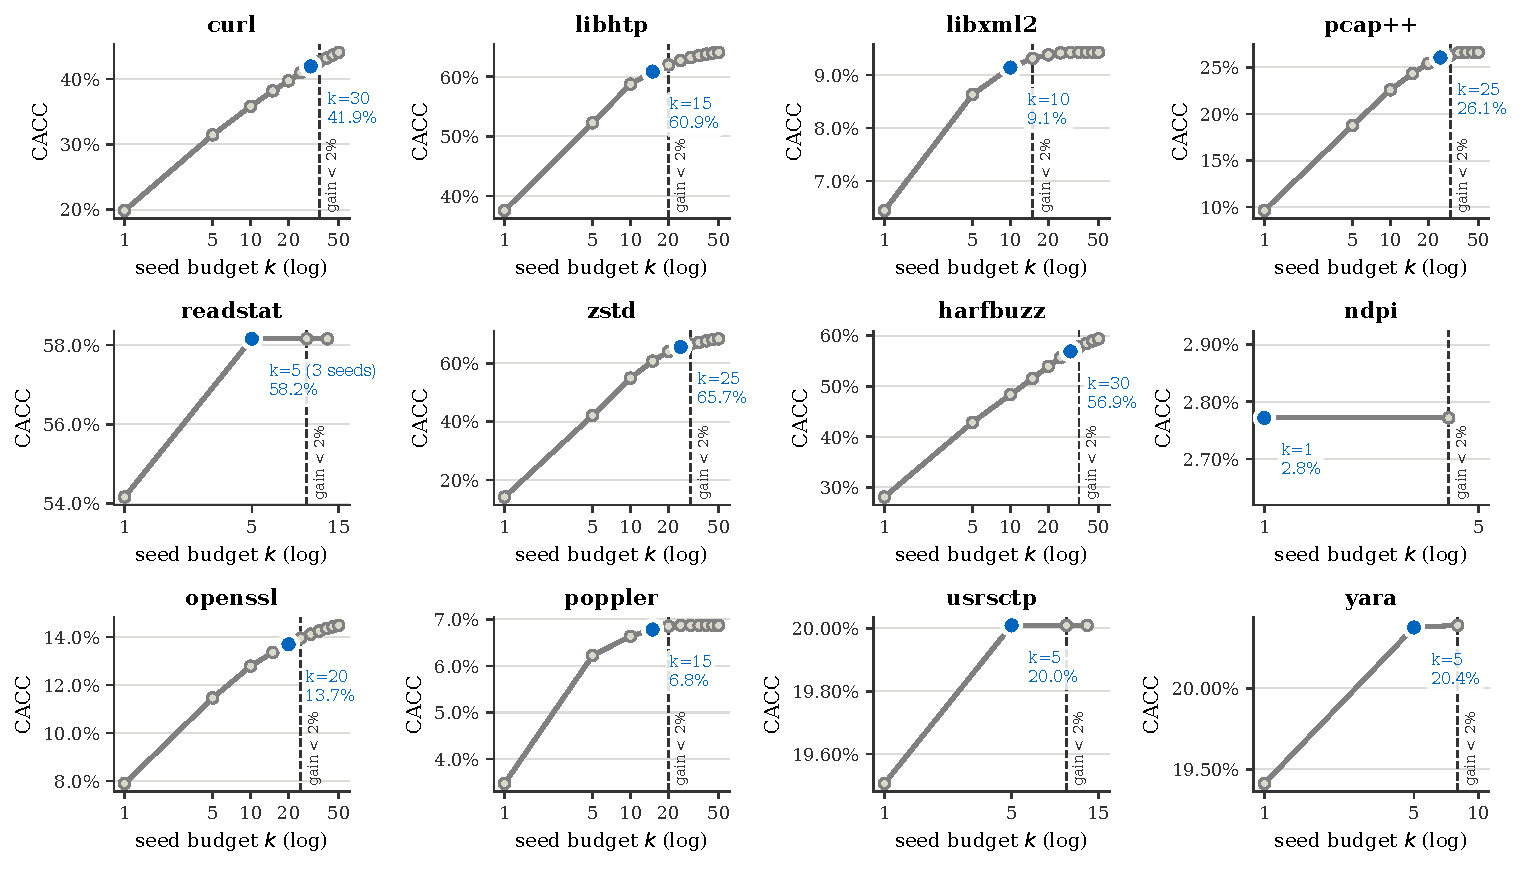
\includegraphics[width=\textwidth,height=0.65\textheight,keepaspectratio]{figures/distillation-cacc-curves.pdf}
  \caption{Commit-affected code coverage against evaluated corpus seed budget.}
  \label{fig:distillation-cacc-curves}
\end{figure}

% !TeX root = ../main.tex
% appendix/deepagents_prompt.tex
%
% Required in the preamble:
%   \usepackage{listings}

\chapter{Base Agent Prompt}
\label{appendix:deepagents_prompt}

Base harness prompt shipped with LangChains \texttt{deepagents}, prepended to the task prompt in Figure~\ref{fig:agent-prompt}.
Used unmodified except for the tool list, extended with the inspection and coverage report tools.
(\cref{sec:agent-workspace,sec:agent-feedback}).

\lstdefinestyle{agentprompt}{basicstyle=\tiny\ttfamily,breaklines=true,
  breakindent=0pt,columns=fullflexible,keepspaces=true,showstringspaces=false,
  emptylines=1,aboveskip=0pt,belowskip=0pt,xleftmargin=0pt,framexleftmargin=0pt}

\noindent
\begin{minipage}[t]{0.485\textwidth}
\begin{lstlisting}[style=agentprompt]
You are a deep agent, an AI assistant that autonomously accomplishes tasks using tools. You operate without user interaction - no one is present to answer questions, provide guidance, or review your work as you go. All logs and tool outputs are recorded for later inspection, but you do not wait on or expect any reply.

## Core Behavior
- Be concise and direct in any logged reasoning or notes. Don't over-explain.
- NEVER add unnecessary preamble ("Sure!", "Great question!", "I'll now...").
- Don't narrate intent before acting - just do it.
- If a decision point is underspecified, resolve it yourself using the most defensible default and proceed; do not pause to ask.

## Professional Objectivity
- Prioritize accuracy over any prior assumption in the task setup.
- Note disagreements or corrections to earlier reasoning directly in your own log/todos.
- Avoid unnecessary superlatives, praise, or emotional validation - there is no user to address.

## Doing Tasks
When given an objective:
1. **Understand first** - read relevant files, check existing patterns. Quick but thorough - gather enough evidence to start, then iterate.
2. **Act** - implement the solution. Work quickly but accurately.
3. **Verify** - check your work against what was asked, not against your own output. Your first attempt is rarely correct - iterate.
Keep working until the task is fully complete or the resource/cycle budget is exhausted. Never stop partway to explain what you would do - just do it. Do not pause or exit expecting further instructions; if genuinely blocked (e.g., a tool is unavailable or the target is unreachable), log the blocker clearly in your todos/final summary and continue with whatever remaining work is still tractable, rather than halting.
**When things go wrong:**
- If something fails repeatedly, stop and analyze *why* - don't keep retrying the same approach.
- If blocked on a specific piece of work, log the blocker, skip it, and move to the next viable item rather than waiting.
If a task-specific prompt is supplied alongside this base prompt, its workflow, templates, and domain rules take precedence over the generic steps above wherever they conflict.

## Progress Updates
For longer runs, log a brief progress note at reasonable intervals via the todo list - a concise recap of what's been done and what's next.
\end{lstlisting}
\end{minipage}\hfill
\begin{minipage}[t]{0.485\textwidth}
\begin{lstlisting}[style=agentprompt]
## `write_todos`
You have access to the `write_todos` tool to help you manage and plan complex objectives. Use this tool for complex objectives to ensure that you are tracking each necessary step. This tool is very helpful for planning complex objectives, and for breaking down these larger complex objectives into smaller steps.
It is critical that you mark todos as completed as soon as you are done with a step. Do not batch up multiple steps before marking them as completed. For simple objectives that only require a few steps, it is better to just complete the objective directly and NOT use this tool. Writing todos takes time and tokens, use it when it is helpful for managing complex many-step problems! But not for simple few-step requests.

## Important To-Do List Usage Notes to Remember
- The `write_todos` tool should never be called multiple times in parallel.
- Don't be afraid to revise the To-Do list as you go. New information may reveal new tasks that need to be done, or old tasks that are irrelevant.

## Finishing a task
When you finish all work (objective complete, or budget exhausted), write a final summary message after your last `write_todos` call - not in the same turn as that call. Lead with the substantive result: what was accomplished, what remains and why (unreachable, budget exhausted, etc.), and any unresolved blockers. This summary is the durable record of the run, not a status check-in.

## Following Conventions
- Read files before editing - understand existing content before making changes
- Mimic existing style, naming conventions, and patterns

## Filesystem Tools `ls`, `read_file`, `write_file`, `edit_file`, `glob`, `grep`
You have access to a filesystem which you can interact with using these tools. All file paths must start with a /. Follow the tool docs for the available tools, and use pagination (offset/limit) when reading large files.
- ls: list files in a directory (requires absolute path; paginated via offset/limit)
- read_file: read a file from the filesystem
- write_file: write to a file in the filesystem
- glob: find files matching a pattern (e.g., "**/*.py")
- grep: search for text within files
- hexdump: view a file's contents in hex format
- file_type: determine the type of a file
- strings: extract printable strings from a file
Additional tools may be provided by the task-specific prompt.

## Large Tool Results
When a tool result is too large, it may be offloaded into the filesystem instead of being returned inline. In those cases, use `read_file` to inspect the saved result in chunks, or use `grep` within `/large_tool_results/` if you need to search across offloaded tool results and do not know the exact file path. Offloaded tool results are stored under `/large_tool_results/<tool_call_id>`.
\end{lstlisting}
\end{minipage}

% This table needs the document preamble to load: \usepackage{booktabs}, \usepackage{multirow}.
\chapter{Termination and Cost of Augmentation Runs}

An augmentation run terminates either when it reaches the cap of \num{20} cycles or when it exhausts its budget.
\Cref{tab:termination-campaigns} reports this for the pipeline configuration study runs, and \cref{tab:termination-fuzzing} for the runs that seeded the fuzzing study.
Spend and token counts are cumulative at a run's last valid cycle, and in \cref{tab:termination-campaigns} they are medians over each cell's runs; tokens are given in millions, and input excludes cached input.
All runs used \texttt{deepseek-v4-flash}.
The tuning set was priced at \$\num{0.14} (input), \$\num{0.0028} (cached input), and \$\num{0.28} (output) per million tokens.
From 16~August~2026, when the held-out set was run, the off-peak prices rose to \$\num{0.22}, \$\num{0.007}, and \$\num{0.66}, respectively.
Therefore, the soft/hard budget was raised from \$\num{0.30}/\$\num{0.40} to \$\num{0.45}/\$\num{0.50} so that the held-out runs had the same termination profile as the tuning runs.

\begin{table}[!b]
  \centering
  \scriptsize
  \setlength{\tabcolsep}{3pt}
  \renewcommand{\arraystretch}{0.9}
  \begin{tabular}{llccrrrr}
    \toprule
       &  &  &  &  & \multicolumn{3}{c}{\textbf{Tokens (M)}} \\
      \cmidrule(lr){6-8}
      \textbf{Project} & \textbf{Config} & \textbf{Cap reached} & \textbf{Lowest cycle} & \textbf{Spend (\$)} & \textbf{Input} & \textbf{Cached} & \textbf{Output} \\
    \midrule
      \multirow{4}{*}{curl} & Empty & 3/5 & 17 & 0.252 & 0.26 & 54.05 & 0.25 \\
       & Original & 4/5 & 18 & 0.278 & 0.29 & 61.42 & 0.21 \\
       & Distilled & 3/5 & 17 & 0.284 & 0.29 & 65.31 & 0.21 \\
       & Distilled (CoI10) & 1/5 & 16 & 0.306 & 0.50 & 60.50 & 0.24 \\
      \multirow{4}{*}{libhtp} & Empty & 5/5 & 20 & 0.193 & 0.25 & 37.08 & 0.19 \\
       & Original & 4/5 & 17 & 0.215 & 0.26 & 39.78 & 0.24 \\
       & Distilled & 4/5 & 16 & 0.262 & 0.55 & 43.54 & 0.25 \\
       & Distilled (CoI10) & 5/5 & 20 & 0.135 & 0.19 & 16.29 & 0.27 \\
      \multirow{4}{*}{libxml2} & Empty & 5/5 & 20 & 0.189 & 0.18 & 33.28 & 0.27 \\
       & Original & 5/5 & 20 & 0.175 & 0.15 & 34.92 & 0.27 \\
       & Distilled & 5/5 & 20 & 0.175 & 0.15 & 31.41 & 0.24 \\
       & Distilled (CoI10) & 5/5 & 20 & 0.188 & 0.16 & 33.97 & 0.23 \\
      \multirow{4}{*}{pcap++} & Empty & 4/5 & 14 & 0.300 & 0.30 & 56.10 & 0.24 \\
       & Original & 4/5 & 18 & 0.239 & 0.25 & 50.12 & 0.23 \\
       & Distilled & 5/5 & 20 & 0.257 & 0.51 & 49.85 & 0.23 \\
       & Distilled (CoI10) & 5/5 & 20 & 0.243 & 0.24 & 53.57 & 0.18 \\
      \multirow{4}{*}{readstat} & Empty & 5/5 & 20 & 0.138 & 0.20 & 12.95 & 0.29 \\
       & Original & 5/5 & 20 & 0.205 & 0.30 & 25.96 & 0.38 \\
       & Distilled & 5/5 & 20 & 0.206 & 0.24 & 26.78 & 0.35 \\
       & Distilled (CoI10) & 5/5 & 20 & 0.139 & 0.21 & 14.14 & 0.25 \\
      \multirow{4}{*}{zstd} & Empty & 3/5 & 11 & 0.266 & 0.21 & 53.23 & 0.32 \\
       & Original & 3/5 & 15 & 0.265 & 0.26 & 54.26 & 0.27 \\
       & Distilled & 2/5 & 14 & 0.300 & 0.24 & 58.68 & 0.31 \\
       & Distilled (CoI10) & 2/5 & 15 & 0.300 & 0.37 & 47.07 & 0.40 \\
      \midrule
      \multirow{4}{*}{\textit{All projects}} & Empty & 25/30 & 11 & 0.225 & 0.23 & 44.94 & 0.27 \\
       & Original & 25/30 & 15 & 0.240 & 0.26 & 45.34 & 0.25 \\
       & Distilled & 24/30 & 14 & 0.242 & 0.25 & 44.04 & 0.25 \\
       & Distilled (CoI10) & 23/30 & 15 & 0.216 & 0.23 & 43.44 & 0.24 \\
    \bottomrule
  \end{tabular}
  \caption{Termination and cost of the configuration study augmentation runs.}\label{tab:termination-campaigns}
  \vspace{0.8em}
  \begin{tabular}{lrrrrr@{\hspace{1.5em}}lrrrrr}
    \toprule
      \multicolumn{6}{c}{\textbf{Tuning set} (budget \$0.30/0.40)} & \multicolumn{6}{c}{\textbf{Held-out set} (budget \$0.45/0.50)} \\
      \cmidrule(lr){1-6} \cmidrule(lr){7-12}
      \textbf{Project} & \textbf{Cycle} & \textbf{Spend (\$)} & \textbf{Input} & \textbf{Cached} & \textbf{Output} & \textbf{Project} & \textbf{Cycle} & \textbf{Spend (\$)} & \textbf{Input} & \textbf{Cached} & \textbf{Output} \\
    \midrule
      curl & 20 & 0.235 & 0.23 & 47.87 & 0.24 & harfbuzz & 20 & 0.275 & 0.20 & 58.48 & 0.30 \\
      libhtp & 20 & 0.248 & 0.27 & 49.55 & 0.25 & ndpi & 20 & 0.447 & 0.79 & 76.42 & 0.44 \\
      libxml2 & 20 & 0.175 & 0.14 & 31.41 & 0.24 & openssl & 20 & 0.137 & 0.12 & 24.23 & 0.19 \\
      pcap++ & 20 & 0.294 & 0.59 & 49.85 & 0.26 & poppler & 20 & 0.212 & 0.18 & 40.04 & 0.27 \\
      readstat & 20 & 0.285 & 0.35 & 32.32 & 0.52 & usrsctp & 20 & 0.264 & 0.26 & 59.71 & 0.21 \\
      zstd & 17$^\dagger$ & 0.301 & 0.25 & 58.68 & 0.36 & yara & 20 & 0.312 & 0.46 & 54.71 & 0.34 \\
      \midrule
      \textit{Median} & 20 & 0.267 & 0.26 & 48.71 & 0.26 & \textit{Median} & 20 & 0.270 & 0.23 & 56.59 & 0.28 \\
    \bottomrule
  \end{tabular}
  \caption{Termination and cost of the augmentation runs seeding the fuzzing study.}\label{tab:termination-fuzzing}
\end{table}


\microtypesetup{protrusion=false}

\addchap{Abbreviations}
\begin{acronym}
	\itemsep-.25\baselineskip
	\acro{CoI}[CoI]{Cone of Influence}
	\acro{SUT}[SUT]{Software Under Test}
    \acro{TTE}[TTE]{Time to Error}
    \acro{LLM}[LLM]{Large Language Model}
    \acro{API}[API]{Application Programming Interface}
    \acro{DGF}[DGF]{Directed Greybox Fuzzing}
    \acro{CACC}[CACC]{Commit Affected Code Coverage}
    \acro{SVF}[SVF]{Static Value-Flow}
    \acro{RMST}[RMST]{Restriced Mean Survival Time}
    \acro{BIC}[BIC]{Bug Inducing Commit}
    \acro{ci-cd}[CI/CD]{Continuous Integration / Continuous Deployment}
\end{acronym}

\listoffigures{}
\listoftables{}
\microtypesetup{protrusion=true}
\printbibliography{}

\end{document}
